\documentclass[12pt,english]{article}
\usepackage[utf8]{inputenc}
\usepackage[a4paper]{geometry}
\geometry{verbose,tmargin=2cm,bmargin=2cm,lmargin=3cm,rmargin=2cm,headheight=12pt,headsep=24pt}
\setcounter{secnumdepth}{4}
\usepackage{titlesec}
\titleformat{\paragraph}
{\normalfont\normalsize\bfseries}{\theparagraph}{1em}{}
\titlespacing*{\paragraph}
{0pt}{3.25ex plus 1ex minus .2ex}{1.5ex plus .2ex}
\setcounter{tocdepth}{3}
\usepackage{pdfpages}
\usepackage{bm}
\usepackage{array}
\usepackage{float}
\usepackage{graphicx}
\usepackage{tocloft}
\usepackage{hyperref}
\hypersetup{
    colorlinks=true,
    linkcolor=blue,
    filecolor=blue,      
    urlcolor=blue,
}
\usepackage{setspace}
\PassOptionsToPackage{normalem}{ulem}
\usepackage{ulem}
\usepackage{indentfirst}	%Az összes címsor utáni bekezdést beljebb viszi%
\usepackage{amsmath}
\usepackage{tikz}
\usepackage{wrapfig}
\usetikzlibrary{shadings}

\usepackage{pgfplots}


\usepackage{hyperref}
\hypersetup{
    colorlinks,
    citecolor=black,
    filecolor=black,
    linkcolor=black,
    urlcolor=black
}




\makeatletter

%%%%%%%%%%%%%%%%%%%%%%%%%%%%%% LyX specific LaTeX commands.
\newcommand{\noun}[1]{\textsc{#1}}
%% Because html converters don't know tabularnewline
\providecommand{\tabularnewline}{\\}

%%%%%%%%%%%%%%%%%%%%%%%%%%%%%% Textclass specific LaTeX commands.
\newenvironment{lyxcode}
{\par\begin{list}{}{
\setlength{\rightmargin}{\leftmargin}
\setlength{\listparindent}{0pt}% needed for AMS classes
\raggedright
\setlength{\itemsep}{0pt}
\setlength{\parsep}{0pt}
\normalfont\ttfamily}%
 \item[]}
{\end{list}}

%%%%%%%%%%%%%%%%%%%%%%%%%%%%%% User specified LaTeX commands.
%\textwidth 160mm
%\oddsidemargin 0cm
%\topmargin -15mm
\usepackage{bm}
\newcommand{\tg}{\mathop\mathrm{tg}}
\newcommand{\grad}{\mathop\mathrm{grad}}
\newcommand{\BME}{\hrule\vspace{6pt}{\large Budapest University of Technology and Economics
\\
Faculty of Mechanical Engineering \\
Department of Applied Mechanics}}
\newcommand{\szerzo}{}
\newcommand{\konzulensek}{
\parbox[t]{20cm}
{\normalsize
\hspace*{25em} Made by:\\
\hspace*{28em}Bálint CSATÓ\\
\hspace*{25em}Supervisor:\\
\hspace*{28em}Gergely GYEBRÓSZKI \\
}\hfill}

\makeatother

\usepackage{babel}


\begin{document}



\title{\vspace{-2cm}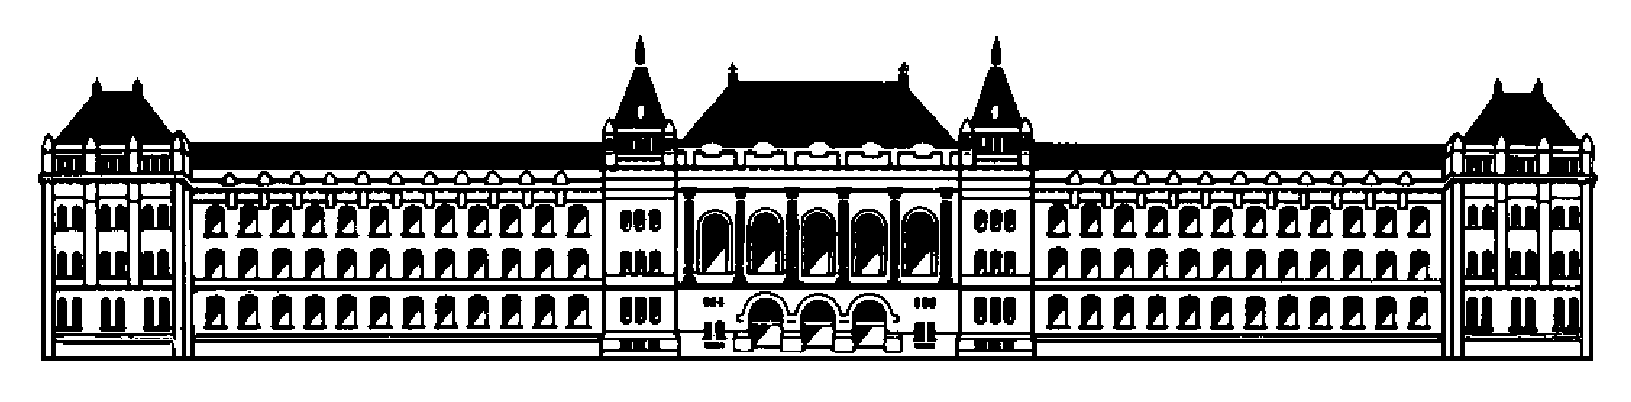
\includegraphics[width=0.4\textwidth,keepaspectratio]{figures/bme_skyline}\\
\BME\vspace{4cm}\\
Control and Parameter Estimation Problems of Autonomous Transport Robots
\\[5mm]
\large{Final Project}}


\author{\sc\szerzo}


\date{\vspace{6cm}\konzulensek\\
\vspace{3cm}Budapest, 2018}

\maketitle
\thispagestyle{empty}



\newpage
\pagenumbering{arabic}
\renewcommand{\contentsname}{Contents}
\renewcommand{\cftsecleader}{\cftdotfill{\cftdotsep}}
\tableofcontents
\numberwithin{equation}{section} % Number equations within sections
\numberwithin{figure}{section} % Number figures within sections
\numberwithin{table}{section} % Number tables within sections

\newpage
%%%%%%%%%%%%%%%%%%%%%%%%%%%%%%%%%%%%%%%%%%%%%%%%%%%%%%%%%%%%%%%%%%%%%%%%%%%%%%%%%%%%%%%%%%%%%%%%%%%%%%%%%%%%
% 													Preface
%%%%%%%%%%%%%%%%%%%%%%%%%%%%%%%%%%%%%%%%%%%%%%%%%%%%%%%%%%%%%%%%%%%%%%%%%%%%%%%%%%%%%%%%%%%%%%%%%%%%%%%%%%%%
\section*{Preface}
Autonomous vehicle technology offers the possibility of fundamentally
changing transportation. Equipping cars and light vehicles
with this technology will likely reduce crashes, energy consumption,
and pollution and reduce the costs of congestion, as well.............
blabalblablalblalba
lablblablablalblballb
labllablblalbalblalblbal

\addcontentsline{toc}{section}{Preface}

\newpage
%%%%%%%%%%%%%%%%%%%%%%%%%%%%%%%%%%%%%%%%%%%%%%%%%%%%%%%%%%%%%%%%%%%%%%%%%%%%%%%%%%%%%%%%%%%%%%%%%%%%%%%%%%%%
% 											Introduction to Autonomous Transport Robots
%%%%%%%%%%%%%%%%%%%%%%%%%%%%%%%%%%%%%%%%%%%%%%%%%%%%%%%%%%%%%%%%%%%%%%%%%%%%%%%%%%%%%%%%%%%%%%%%%%%%%%%%%%%%
\section{Introduction to Autonomous Transport Robots}
\subsection{History of transportation}

Since the early days of the human civilization, one of the most common problem has been the transportation. The first major development was the domestication of animals what made it possible to transport more and heavier loads or humans themselves in order to achieve greater speed and duration. The next substantial invention was the wheel which increased the efficiency of animal transport introducing the concept of vehicles. Until the Industrial Revolution, the water transport facilities proved to be the most effective way. With the development of the combustion engines and automobiles around the end of the $19^{st}$ century, road transport became competitive again. Today trucks transport cargos over thousands of miles, but light items are still being carried in wheelbarrows or trailers attached to more compact vehicles. 

\begin{figure}[h]
	\centering
	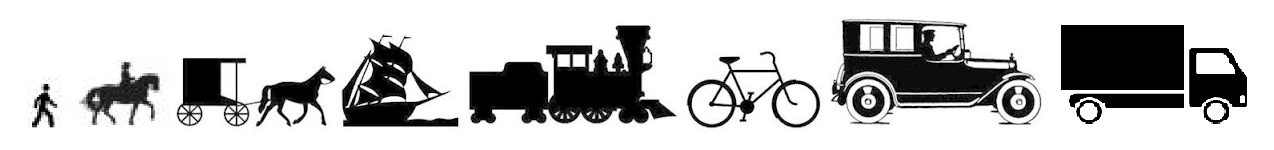
\includegraphics[width=10cm]{figures/evot}
	\label{fig1}
	\caption{Evolution of Transportation}
\end{figure}

\noindent One of the most dominant development tendency in almost every field of the industry is the automation of processes and procedures. Automation means the reduction of human intervention in the operation of machines. The benefit of automation include labor savings, savings in electricity costs, savings in material costs, and improvements to quality, accuracy and precision. The most trending application of the automation regarding the transportation is the autonomous cars on the roads. 
\subsection{Autonomous vehicles}
An autonomous car which is also known as a self-driving car or a driverless car, is a vehicle that can operate without a certain amount of human control using its sensors to monitor the informations coming from the environment. Great variety of techniques are used to detect the surroundings, such as radar, laser light, GPS, odometry and computer vision. The collected information provides a decent input to the control system which is the soul of the self-driving cars. Several control problems have to be solved continuously during driving on the roads, such as identifying obstacles and avoiding them, following transportation rules or navigating along a predefined path.

Autonomous vehicle technology offers the possibility of fundamentally
changing transportation. Equipping cars and light vehicles
with this technology will likely reduce traffic collisions, thus the resulting injuries and the related costs including less need for insurance. Autonomous cars are predicted to increase the traffic flow and the mobility of citizens. Reduced traffic congestion and the improvements in traffic flow due to widespread use of autonomous cars will also result in better fuel efficiency and reduced pollution in cities.

In spite of the various benefits also several issues exist such as technology challenges, disputes concerning liability, customer concerns about the safety of driverless cars, risk of loss of privacy and security concerns against hackers, risk of negative effects on the society and economy and finally moral issues when car's software is forced to choose between multiple harmful alternatives during an inevitable accident. \cite{wiki}
 

The autonomous driving technology can be most easily conceptualized using a five-part
continuum suggested by the National Highway Traffic Safety Administration
(NHTSA), with different benefits of the technology realized
at different levels of automation:
\begin{itemize}
	\item \textbf{Level 0:}  The human driver is in complete control of all functions of the car.
	\item \textbf{Level 1:}  One function is automated.
	\item \textbf{Level 2:}  More than one function is automated at the same time (e.g., steering and acceleration), but the driver must remain constantly attentive.
	\item \textbf{Level 3:} The driving functions are sufficiently automated that the driver can safely engage in other activities.
	\item \textbf{Level 4:} The car can drive itself without a human driver.\cite{c}
\end{itemize}
\noindent

From engineering point of view, the most important issues are the technological challenges, i.e. how to design a driverless vehicle system which is capable of handling vehicle's performance like human in all possible conditions. An autonomous vehicle is a combination of sensors and actuators, sophisticated algorithms executed as a software on a processor.
The sensory system can be classified into three different classes:
\begin{itemize}
	\item \textbf{Navigation and guidance:} the system which determines – where you are, where you want to go, and how do you get there. In the most common applications different techniques such as GPS, compass and dead reckoning are used.
	\item \textbf{Driving and Safety:} Directing the vehicle and making sure that vehicle follows the rules of the road. The autonomous car must be able to see and interpret what is in front of it when it is going forward (and behind when in reverse). It is also necessary to see what is on either side, in other words, it needs a 360$^{\circ}$ view. A set of video cameras is an obvious choice by which location of lanes and surrounding objects or markers on the road can determined.
	\item \textbf{Performance:} managing car's internal system. Several application specific, unique circuit boards and subsystems are added to a conventional vehicle to provide the functions needed for autonomous operation. Much of the system-level operation involves measuring and managing the power requirements to control power, overall consumption, and thermal dissipation.
\end{itemize}

The concept of driverless cars made a lot of attention over the past ten years. Generally speaking it can be said that one of the most determining development directions in the automotive industry are related to automated solutions. Many people still do not believe that there could be such a possibility with fully driverless vehicles due to the fact that there so many parameters in the driving function that have to be controlled simultaneously and continuously and even a single failure could cause catastrophy. Nowadays after a lot of research and experiments self-driving cars can be seen as a reality, or at least close future. Still, there are many challenges in designing a fully autonomous system for a self-driving car. The challenges of driverless cars can be sorted into five groups:

\begin{itemize}
	\item  \textbf{Road conditions:} 
	Road conditions can be unpredictable and varying, i.e. in some cases they are smooth and well-marked while in other cases there are no lane marking. On some roads there can be potholes, in case of mountainous and tunnel roads the visibility of external signals for direction are poor.
	
	\item 	\textbf{Weather conditions:}
	It can be sunny and clear or rainy and stormy weather. Autonomous cars have to work in all weather conditions, there is no scope for any failure.
	
	\item \textbf{Traffic conditions:}
	Maybe this is the most complex problem as the human behaviour and autonomous car algorithm have to be matched with each other. The cars would have to drive in all sorts of traffic conditions as humans can do it. The people are emotional beings operating irrationally sometimes. Beside the fact that the traffic would be highly self-regulated, in certain cases some people might break the rules resulting an unpredictable situation in point of a self-driving car. An object may turn up in an unexpected conditions, e.g. crashed car which have to be bypassed ignoring some traffic rules. It can be handled by humans easily but for an artificial intelligence it is a harder task as its operation is ruled by rule-following conditions and this kind of situation needs the capability of detecting the need to ignore the rules in that specific case. The lack of intelligence of several autonomous cars on the roads could result in traffic deadlock.
	
	\item \textbf{Accident Liability:}
	One of the most important aspect of autonomous cars is accidents liability. Who is liable for accidents caused by a self-driving car?
	Generally, the software will be the main component that will drive the car and will make all the good and bad decisions. At initial levels of design there is a person who is physically behind the steering wheel and can take over the control, but in newer designs does not have even any dashboard, pedals and steering wheel. In such cars the driver, who is actually almost just a passenger cannot be the liable for an accident. Furthermore, due to the nature of autonomous cars, the drivers can be supposed to be in a relaxed state without paying sufficient attention to handle unexpected traffic conditions, thus by the time they need to act, it may be too late.
	
	\item \textbf{Radar Interference:}
	Autonomous cars use lasers and radar for navigation. The principle of radar works by detecting reflections of radio waves from surrounding objects. The time taken for the reflection is measured to calculate the distance between the car and the object and appropriate action is then taken based on the radar readings. The problems will come up when thousands of cars on the roads try to use the technology because the reflected radar signals can interfere making it difficult to distinguish which signal was emitted by which vehicle. Even if choosing a different radio frequency can eliminate the issue, the available frequency range is unlikely to be sufficient for all the vehicles manufactured.
	\cite{5c}
\end{itemize}
As a conclusion it can be stated that there are still lot of challenges beside the fact that there have been already some autonomous cars on the roads nowadays, but mostly for development and research purposes. Probably, the collective effort of the industry will definitely make the autonomous car in everyday life a reality one day because the benefits are considered to be remarkable. The most important expected benefit would be the reduction of losses of live in road accidents. Benefits with secondary importance are the reduction of fuel consumption, therefore the environment pollution caused by the vehicles, furthermore time and cost savings could be realized due to optimized behaviour. Time, cost and energy savings are top wanted purposes in almost every field of industry and everyday life, therefore autonomous solutions with such desired features will likely appear in more and more applications. 

\subsection{Application of autonomous transport robots}
The conventional ways of transporting could be appropriate for most of the cases but not in those when repeated passages to specific locations in small distances have to be taken.
One of the latest trends in technology is to create such driverless robots that can help people in their everyday life, i.e. bringing any kind of products to customers. A company called Starship launched a several self-driving robotic vehicles on the streets of Washington, D.C. that can transport food and other small items to customers ordering via app.
\begin{figure}[h]
	\centering
	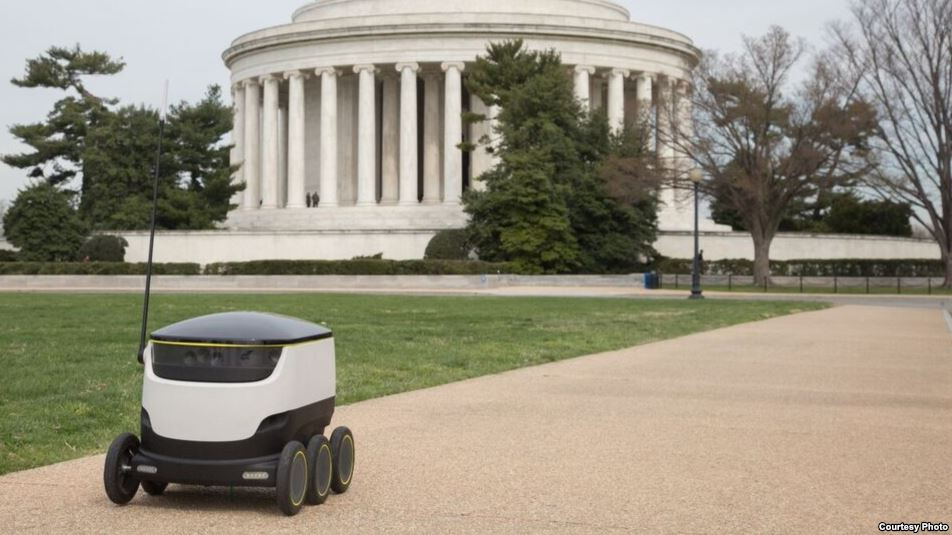
\includegraphics[width=7cm]{figures/starship.jpg}
	\label{fig1}
	\caption{Starship Technologies}
\end{figure}
The robotic vehicles move themeselves along sidewalks using camera and tracking technology to avoid any obstacle and its location can be tracked from the distance in order to know the time of arrival. The six-wheeled electric machine sits about a half-meter high having a lockable cargo bay to carry food products up to nine kilograms in weight.\cite{starship}




A company called SMP Robotics made automated guided vehicles that can remove grass clippings and fallen leaves or construct garbage collection in a garden. 
\begin{figure}[h]
	\centering
	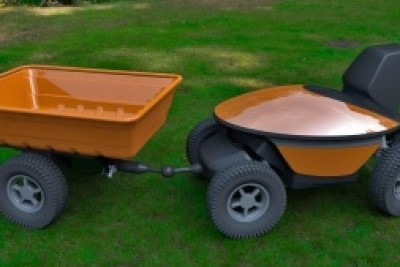
\includegraphics[width=7cm]{figures/smp.jpg}
	\label{smp}
	\caption{SMP Robotics}
\end{figure}

\noindent These small-sized mobile robots have a trailer attached to the back. They are powered by electrical engines, thus noise and smell emission is minimized which allow for operation around people. The built-in accumulators stores the needed energy and can last for several days of cyclical operation. Two ways of route following methods are available. The first option is to choose a root in advance with the help of the attached PC tablet. The second way is to set the robot in its 'follow me' algorithm whereby it is going to follow the operator and learn the path. The collected goods on the trailer can be unloaded automatically using a mechanism without any human intervention. The trailer can be fitted with a water tank which can be used for watering of grass and other plants, furthermore automatic water refill algorithm is implemented. This kind of automatic self-moving watering system suits really well such occasions when a fixed irrigation systems are not worth being built due to climate characteristics.\cite{smp}

A firm named NEOBOTIX made autonomous transport systems for daily use in industrial applications. The robots are equipped with laser scanners that permanently detect landmarks and obstacles what allows the robot to react dynamically to unexpected changes of their surrounding, i.e. to safely operate between human and other moving objects. This flexibility makes them suited for dynamic transportation tasks with frequent changes. For instance, they can complement roller or belt conveyors and take parts to machines or workplaces that are not connected to the conveyor system. \cite{neo}

\begin{figure}[htb!]
	\centering
	\minipage{0.50\textwidth}
	\centering
	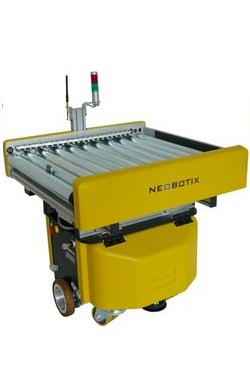
\includegraphics[height=5cm]{figures/neo1.jpg}
	\caption{{\small MT-400}}
	\endminipage\hfill
	\minipage{0.50\textwidth}
	\centering
	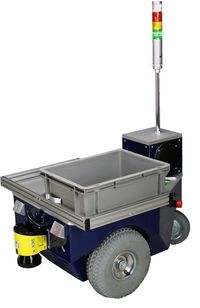
\includegraphics[height=5cm]{figures/neo2.jpg}
	\caption{{\small MT-500}}
	\label{conv2}
	\endminipage\hfill
\end{figure} 

\noindent Possible applications are taking parts to and from workplaces, transporting in direct interaction with humans or dynamic picking of parts for later assembly

BMW logistics also uses autonomous transport robots similarly in industrial environment. The well-known car manufacturer has been working hard to reduce emissions in all steps of the manufacturing process of a car, not only in the final product. This application shows really well that the autonomous developments in the automotive industry is not just about the autonomous driving on the roads but the manufacturing processes as well. Smart Transport Robots (STR) transport components through logistics at the Wackersdorf plant. They measures the distance to wireless transmitters which are located at in the logistics hall to calculate its exact position and route. Using sensors to identify and react to critical situations, it is able to share the route with humans and other vehicles. \cite{bmw}

\begin{figure}[htb!]
	\centering
	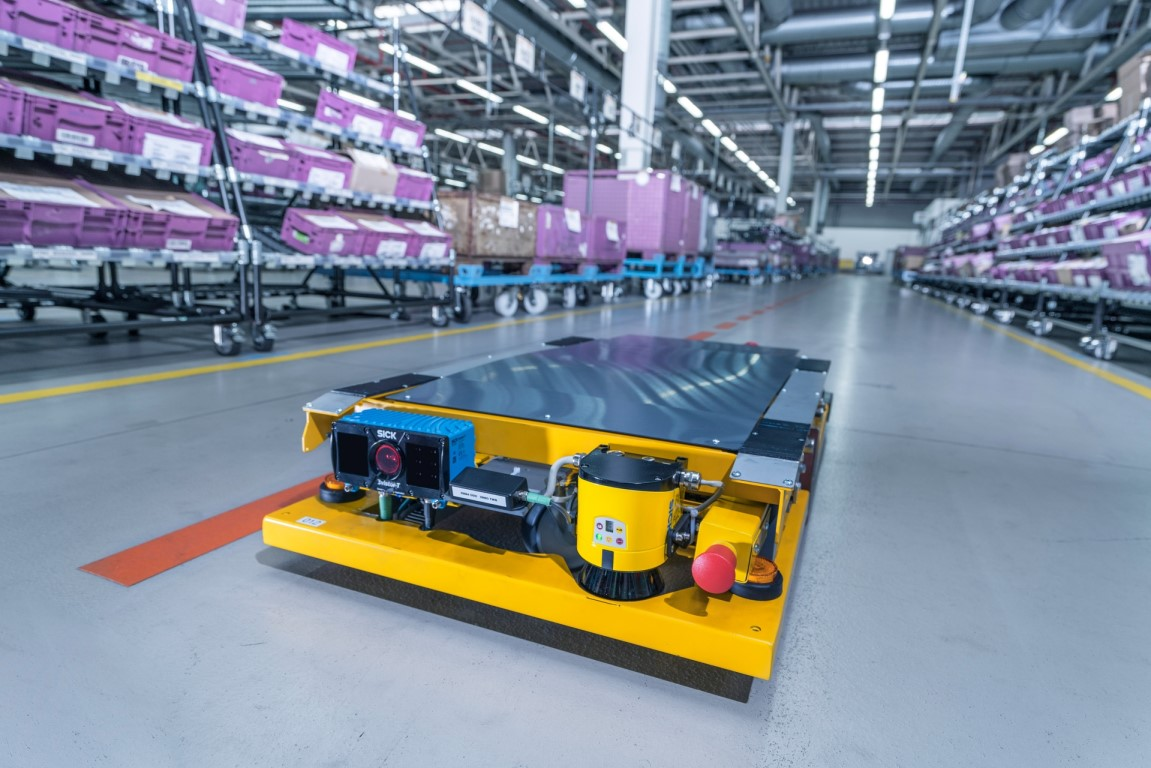
\includegraphics[width=9cm]{figures/bmw.jpg}
	\label{bmw}
	\caption{BMW: Smart Transport Robots}
\end{figure}

A company, named AETHON, made fully autonomous robot called TUG that automates the transport of materials and supplies in commercial environments. It can automatically drop off and pickup of carts, navigates on internal map of facility using laser and it has a omnidirectional 4 wheel driven drive system for higher maneuverability.

\begin{figure}[htb!]
	\centering
	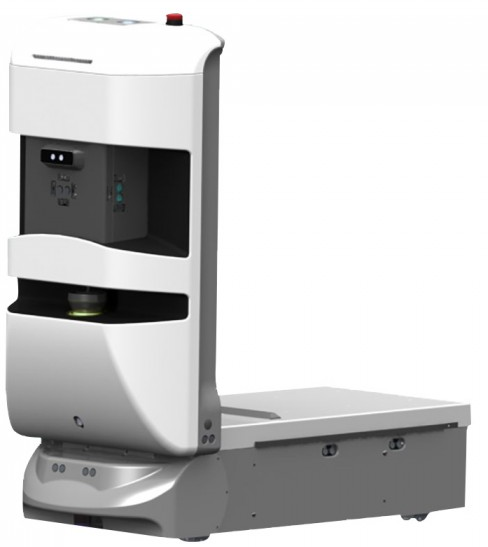
\includegraphics[width=7cm]{figures/tug.png}
	\label{bmw}
	\caption{AETHON: TUG mobile transport robot}
\end{figure}

Another interesting field of application of transportation robots is the military. By putting humans to this work they are often exposed to a risk that could be avoided. The Autonomous Platform Demonstrator is a military transportation robot developed by the U.S. It has a hybrid-electric drive train with six in-hub electric motors powered by li-ion batteries charged using an on-board diesel generator. 

\begin{figure}[h]
	\centering
	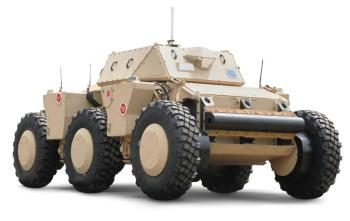
\includegraphics[width=7cm]{figures/apd.jpg}
	\label{bmw}
	\caption{Military transportation robot: APD}
\end{figure}

From control point of view it can be controlled in real-time by a soldier or it can operate autonomously. Autonomously it can operate at speeds up to 50 mph. Furthermore, it can travel along a GPS way point route and avoid obstacles in its way. \cite{apd}






\newpage

\section{Mobile Robots}
The general platform of the transportation robots is obviously the family of mobile robots. Generally a mobile robot faces more design challenges compared to robots that operates in fixed positions as it is left alone in the world. The most critical design problem is related to the locomotion which has to be suited with the conditions of the given ground. In order to handle the changes of the environment and to be able to make decisions during runtime as function of actual state, the robots need to have more intelligence and self-determination. The mobile robots are still not reliable enough nowadays to operate in wide ranges outside of laboratory walls. They need to have a built-in model about their environment, furthermore they need to detect and analyse that of changes and their actual positions have to be found in order to be able to design and perform the next movements. In other words, a sequence of intelligent acts are expected to carry out based on interactions with the dynamically changing outside world.
\subsection{Classification of mobile robots {\normalsize \cite{sieg}\cite{rirt}}}
\subsubsection{Based on the medium in which the robot moves}
\begin{itemize}
	\item \textbf{Air/Space} \\
		These are mostly applied in space flight and military. The most well known application is the Unmanned Aerial Vehicle (UAV), commonly known as drone, which is an aircraft without pilot. The drones develop fast as they are easier to build and control as they do not have to navigate between obstacles.
	\item \textbf{Water} \\
		Automated Underwater Vehicles (AUV) are generally used in seas and oceans for research and industrial purposes. One of the most interesting field is the development of amphibious vehicle that can operate either on earth or on water.
	\item \textbf{Earth} \\
		As it is our natural habitat, the robots operating on earth are the most common.	
\end{itemize}
\subsubsection{Based on the locomotion mechanism}
Mobile robots generally locomote either using wheeled mechanism, a well-known human technology for vehicles, or using a small number of articulated legs being inspired by biological systems. In general, legged locomotion requires higher degrees of freedom and therefore greater mechanical complexity than wheeled locomotion. Wheels, in addition to being simple, are extremely well suited to flat and hard ground, thus their energy need is radically less compared to legged locomotion. However, the softer the surface, the higher the rolling friction which results a dramatic efficiency loss in case of wheeled robots. The efficiency of wheeled locomotion depends on the flatness and hardness of the ground, while the efficiency of legged locomotion depends on the leg mass and body mass. The nature prefers the legged locomotion since they must operate on rough and unstructured terrain where a wheeled vehicle could get stuck easily, e.g. in case of Sojourner Mars rover in 1997. They are simply unable to step over an obstacle, the only chance is to avoid it.
On the other hand, it is also understandable the most of the industrial applications of mobile robotics utilize some form of wheeled locomotion due to the fact that the human environment mostly consists of smooth surfaces, both indoors and outdoors. In such conditions, the wheeled configurations are currently faster and more mobile.

In locomotion, the environment is fixed and the robot moves by imparting force to the environment. The scientific basis is the study of actuators that generate interaction forces and mechanisms that implement the desired kinematic and dynamic properties. The core issues that are need to be evaluated to analyse a robot configuration in terms of locomotion are the followings:
\begin{itemize}
	\item Stability
		\begin{itemize}
			\item number and geometry of contact points
			\item center of gravity
			\item static/dynamic stability
			\item inclination of terrain
		\end{itemize}
	\item Characteristics of contact
		\begin{itemize}
			\item contact point/path size and shape
			\item angle of contact
			\item friction
		\end{itemize}
	\item Type of environment
	\begin{itemize}
		\item structure
		\item medium, (e.g. water, air, soft or hard ground)
	\end{itemize}

\end{itemize}


\subsection{Legged Mobile Robots}
Legged mobile robots contact the ground by a set of contact points which provides good adaptability and maneuverability in rough terrains. Not even the ground quality is an issue until the ground clearance is possible to be maintained, e.g crossing holes which does not exceed the size of the robot is a solvable demand. The main disadvantages of legged systems include power and mechanical complexity. The leg must be capable of sustaining the part of the robot’s total weight, lifting and lowering the robot body meanwhile keeping the stability permanently. Furthermore, high maneuverability needs sufficient number of degrees of freedom to impart forces in a sufficient number of different directions.
The legged robots are basically biologically inspired based on the fact that they are successful locomotion systems. A number of different leg configurations have been successful in a variety of organisms, i.e. the most common numbers are the two, four or six.

\begin{figure}[h]
	\centering
	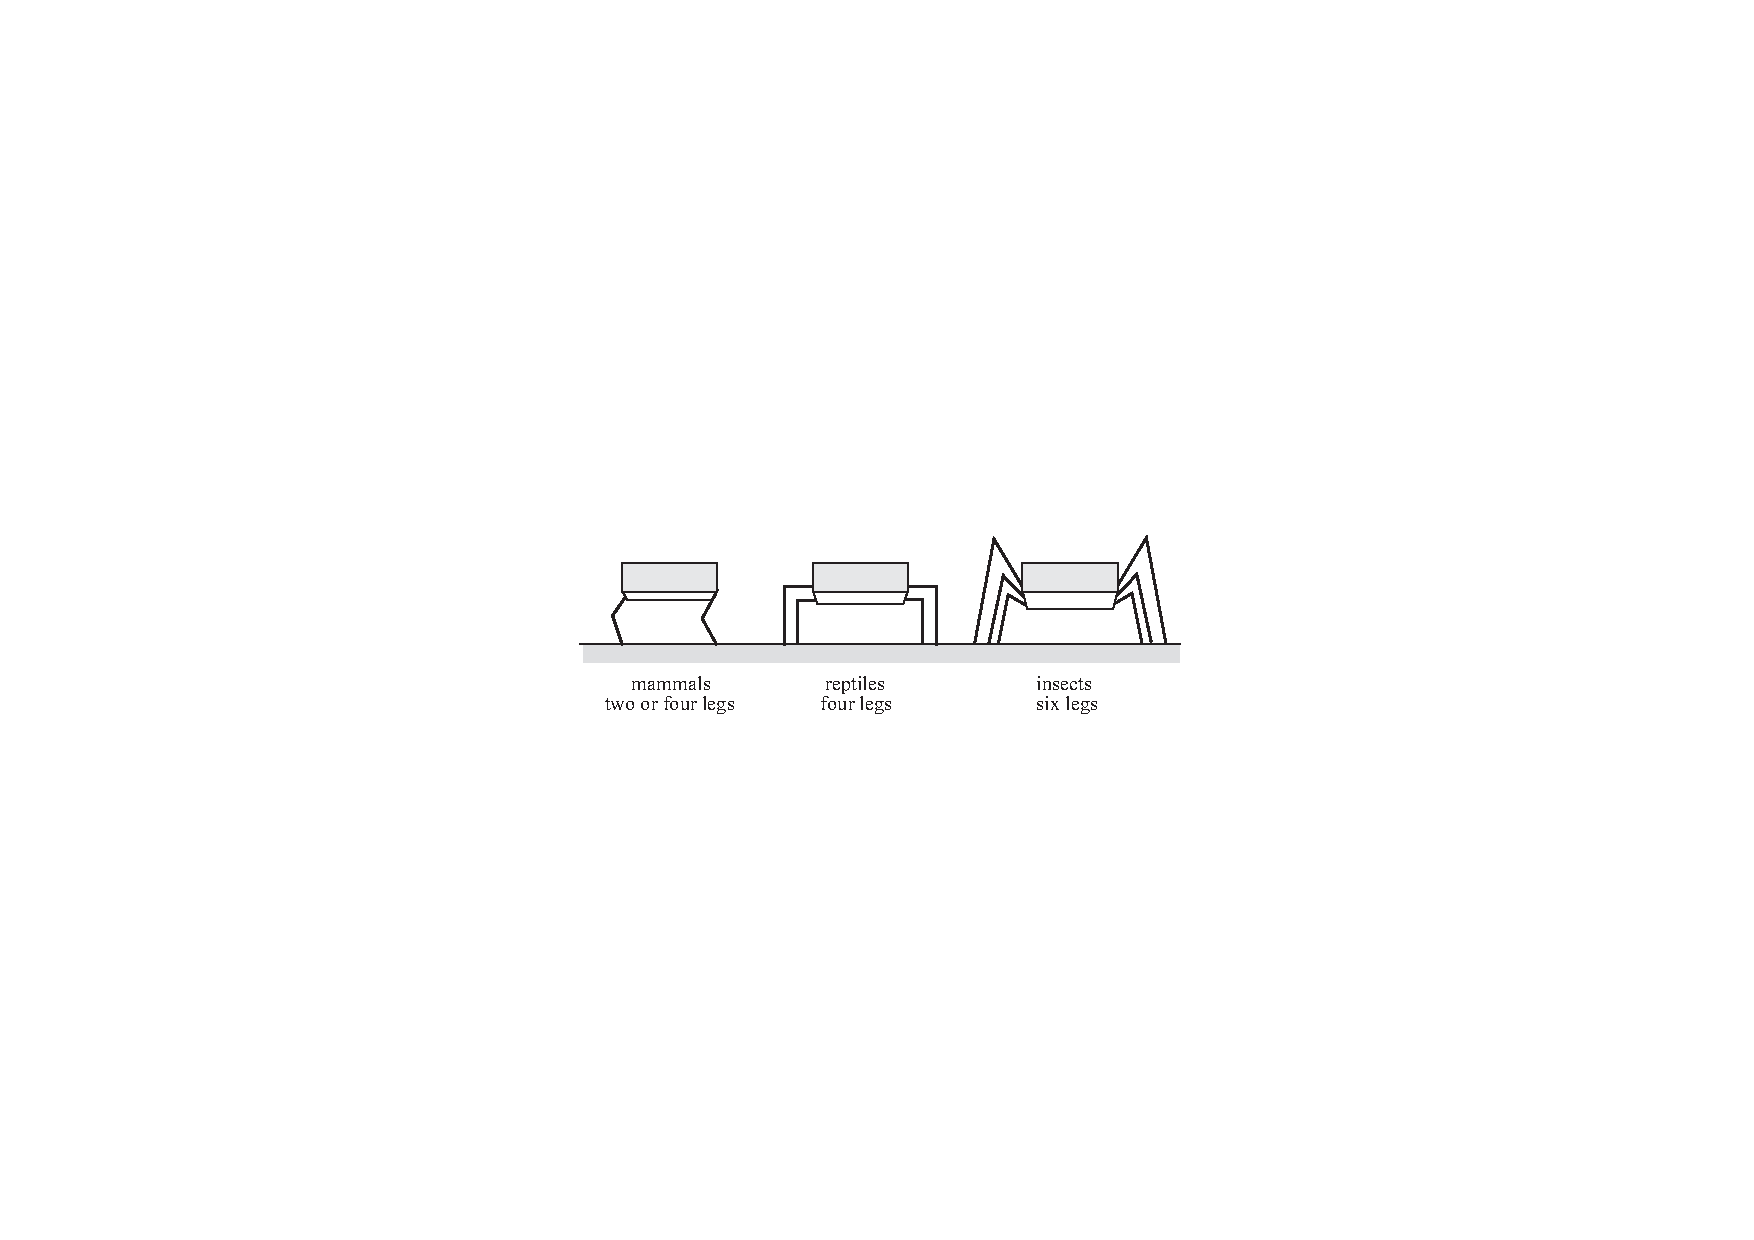
\includegraphics[width=7cm]{figures/legged2.pdf}
	\label{legged}
	\caption{Arrangement of the legs of various animals}
\end{figure}

A creature with at least three legs can achieve static balance which means that no correcting movements have to be taken to preserve its balance. Actually static balance means that the center of gravity is within the tripod of ground contact. A small deviation from stability is passively corrected toward the stable pose by constrain forces after the disturbance goes away. However, any creature who is intended to walk must be able to lift and then release their legs, thus for static walking the minimum number of needed legs is six. Insects and spiders are immediately able to walk when born compared to mammals with four legs who are not able to walk or even to stand in case of humans with only two legs. Therefore the main issue regarding the locomotion of legged robots is the balancing. Of course, the number of legs and also the number of degrees of freedom of a given leg can be increased in order to achieve better stability and maneuverability. On the other hand, more legs and joints result more actuators, thus more energy, more mass, more control, i.e. more costs in certain senses. Most of the legged robots in research and industrial cases have two legs.
The robot legs and arms are usually driven by electrical motors and pneumatic pistons. High level of harmony of the piston movements must be carried out by the designer in order to its hold balance also during the walking what is challenging control task.

\subsection{Wheeled Mobile Robots}
The wheels are the most widely used locomotion mechanisms in man-made vehicles in general due to its simplicity, effectiveness. In most of the cases, during the design the robot builders need to focus problems regarding traction, stability, maneuverability and control. 

\begin{figure}[h]
	\centering
	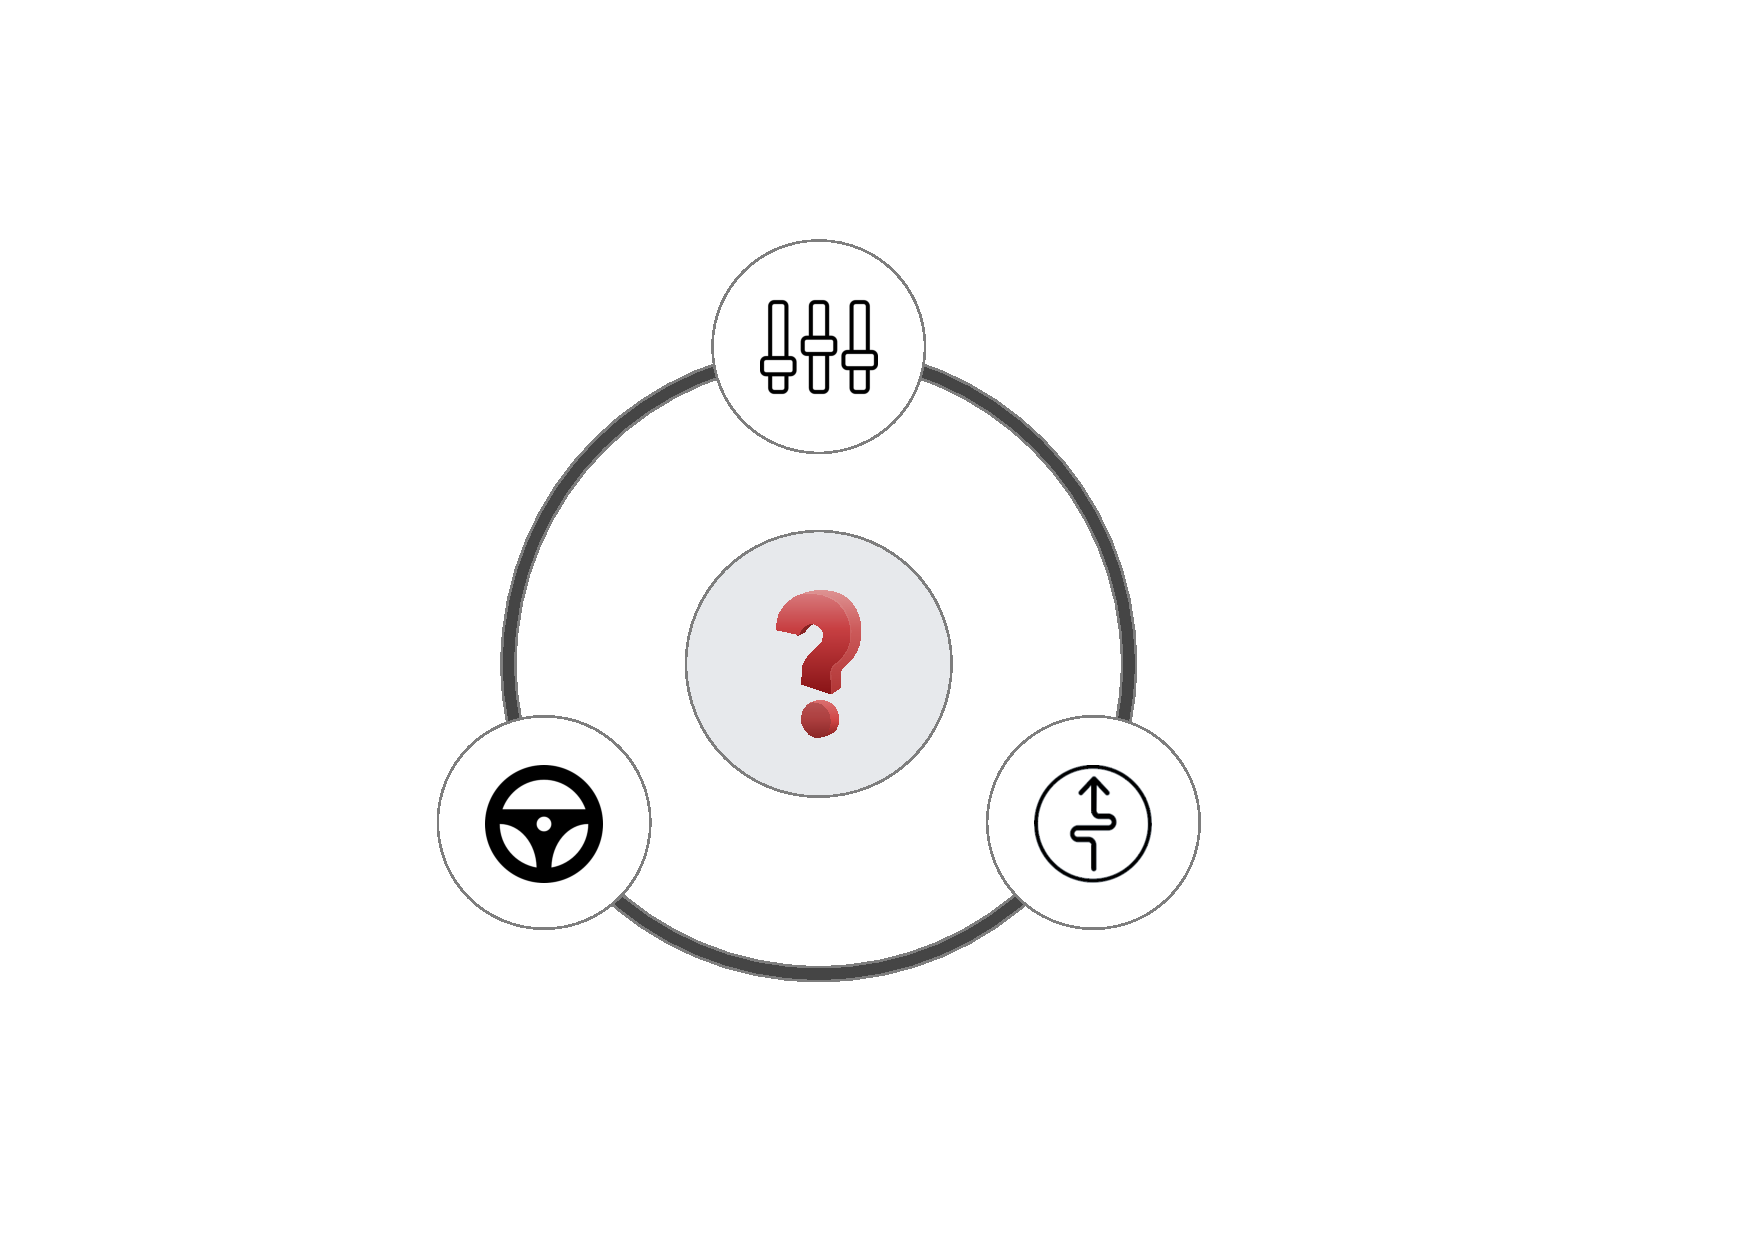
\includegraphics[width=4cm]{figures/triangle.pdf}
	\label{triangle}
	\caption{Major aspects of wheeled robot design}
\end{figure}

In general, balance is not usually an issue in wheeled robotics as they are designed such a way that the all wheels are in contact with the ground. Having three wheels is sufficient to guarantee the static stability if the center of gravity is within the triangle formed by three contact points. Obviously in case of two wheels, self-balancing is necessary. When more than two wheels are used, once the stability improved by adding more contact possibilites, but also a flexible suspension system is required to allow all wheels to maintain ground contact when the robot encounters uneven terrain. One of the simplest approaches to suspension is to design flexibility into the wheel itself, i.e. applying deformable tire of soft rubber material.

Basically, the maneuverability of a given robot depend on the design, the configuration and the degrees of freedoms of powered wheels. Each configuration, wheels type has their advantages and disadvantages that have to be considered before building a mobile robot, we shall see the details later. The robot arrangements can be classified into two groups: holonomic and anholonomic. A mechanical system is called anholonomic if in a specific configuration (state) there exists such displacement or rotation that cannot be carried out by means of the combination of possible actuators. A well known example, an automobile cannot move perpendicular to its orientation because of the kinematic constrains of the wheels. On the other hand, some robots are holonomic, in other words omnidirectional, meaning that they can move at any time in any direction along the ground plane (x,y) regardless of the orientation of the robot around its vertical axis. This level of maneuverability requires wheels that can move in more than just one direction, we shall see the detauls later too.

There is generally an inverse correlation between controllability and maneuverability. For example, the omnidirectional designs require significant processing to convert desired rotational and translational velocities to individual
wheel commands. Furthermore, such omnidirectional designs often have greater degrees of freedom at the wheel. Controlling an omnidirectional robot for a specific direction of travel is also more difficult and often less accurate when compared to less maneuverable designs.

As conclusion, there is no perfect robot configuration that simultaneously maximizes stability, maneuverability, and controllability. For that reason, it is always the designer's task to choose the most appropriate mobile robot configuration considering the constraints originated from the given application.


\subsubsection{Wheel design}
The choice of the wheel type has a large effect on the overall kinematics. There are four major wheel classes as shown in the figure below.
\begin{figure}[h]
	\centering
	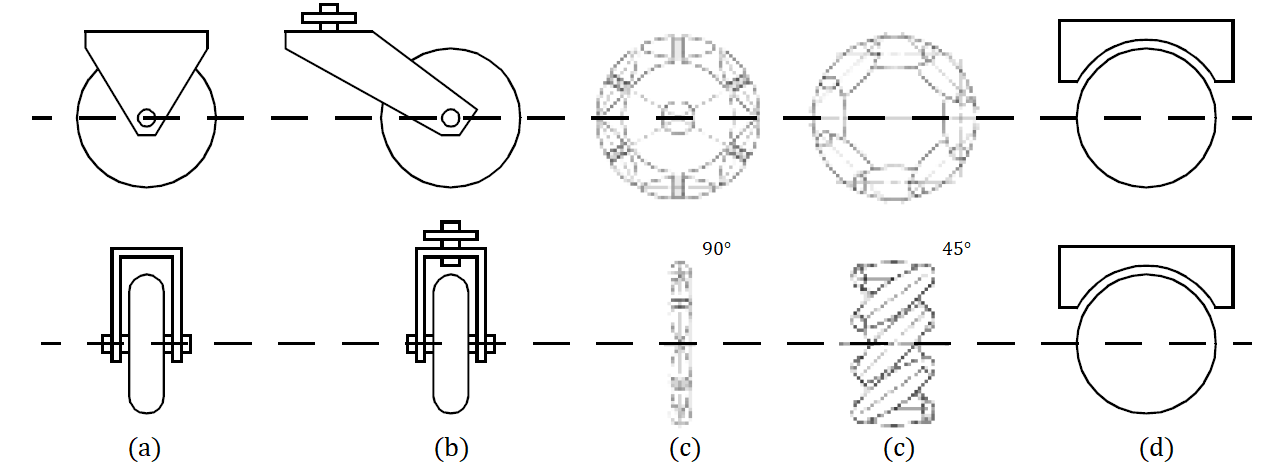
\includegraphics[width=7cm]{figures/wheels4.png}
	\label{wheels}
	\caption{Major classes of wheels: 
		(a) Standard wheel, (b) Castor wheel, (c) Swedish wheel (45$^{\circ}$/90$^{\circ}$), (d) Ball wheel}
\end{figure}
The standard and castor wheel have are highly one-directional as they have a primary axix around they can rotate. These wheels must be steered along a vertical axes to move in a different direction. The main difference between the two configuration is that the castor wheel rotates around an offset vertical axes causing adverse force imparted to the case compared to the standard wheel case where the axes of rotation passes through the contact point. Both the Sweedish and the spherical wheel are less directionally constrained than the former conventional ones. The Swedish wheels functions such as normals wheels providing low resistance in another direction as well, i.e. rolling resistance instead of sticking. Small rollers are attached around the circumference can rotate only in a passive way while the primary axes are the only powered joints. As a result, although the wheel can be driven along only one principal axis, the wheel can move along almost any trajectory. The spherical wheel is a truly omnidirectional wheel, often designed so that it may be actively powered to spin along any direction.

\subsubsection{Wheel configurations}
\paragraph{Holonomic robots}
In practical applications, holonomic systems are rarely present due to higher prices and mechanical complexity, moreover dead reckoning by means of odometry is quite inaccurate. \\[10pt]
\noindent \textbf{Three wheeled omnidirectional mobile robot} \\
The mechanically simplest holonomic robot is omnidirectional configuration. At least three independently driven wheels are needed to be able to move in any direction $(x,y,\varphi)$ in ground plane at any time.
\begin{figure}[htb!]
	\centering
	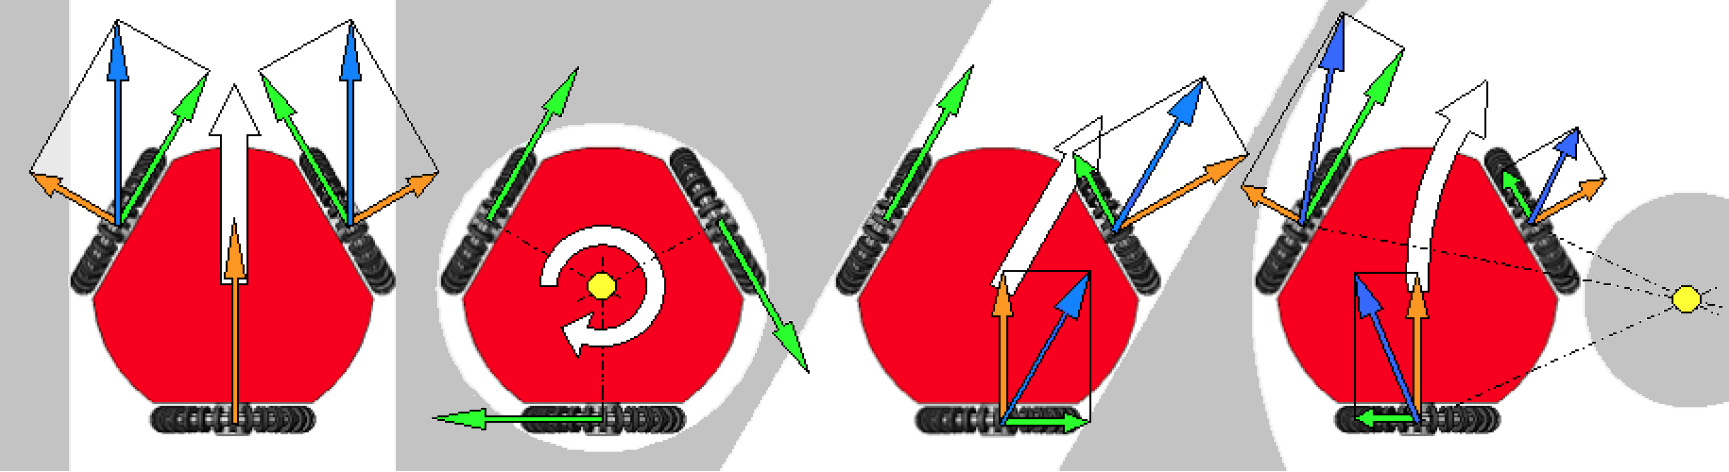
\includegraphics[width=15cm]{figures/omniconfig.png}
	\caption{Three-wheeled omnidirectional drive configuration}
	\label{omniconfig}
\end{figure}
The resultant velocity vectors in terms of wheel velocities can be seen in Figure \ref{omniconfig}. The blue wheel velocity vectors can have lateral component, i.e. the wheels have to be able to move parallel to their primary axes. This kind of configuration needs the previously mentioned Swedish wheels or spherical wheels. 
In addition, also four wheels or even more can be built-in in a system, but in this case it can occur that the wheels drive each other in reverse direction, furthermore the more than three contact point does not guarantee the proper contact of each wheels with the ground.\\[10pt]
\noindent \textbf{Omnidirectional robot with four Swedish wheel} \\
Four-wheeled arrangement with 45$^{\circ}$ Swedish wheels, each driven by a separate motor, have been used in several research and industrial projects. A good example is is Uranus that can rotate and translate independently without any constraints by means of omnidirectional wheels.
\begin{figure}[htb!]
	\centering
	\minipage{0.47\textwidth}
	\centering
	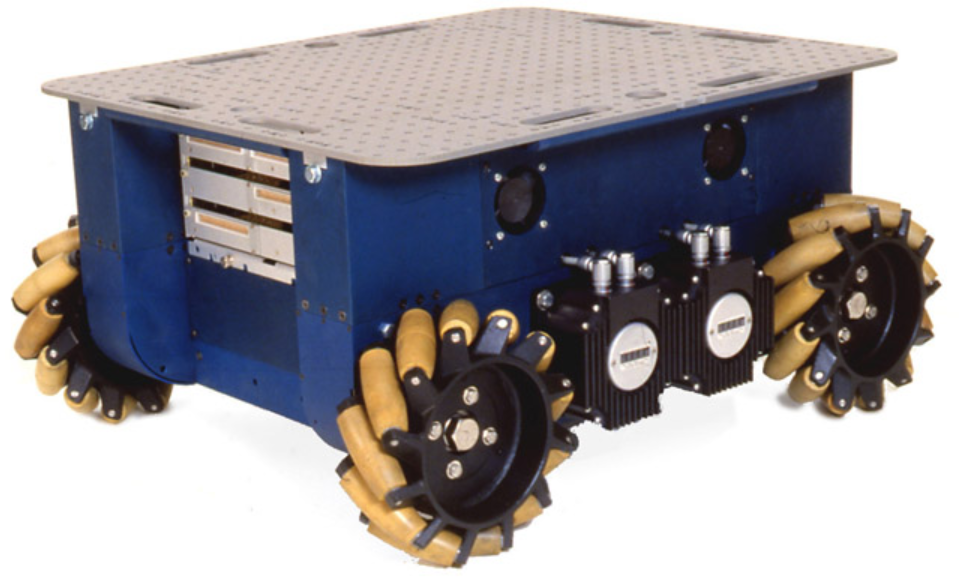
\includegraphics[height=3cm]{figures/uranus}
	\caption{Carnegie Mellon Uranus robot}
	\endminipage\hfill
	\minipage{0.53\textwidth}
	\centering
	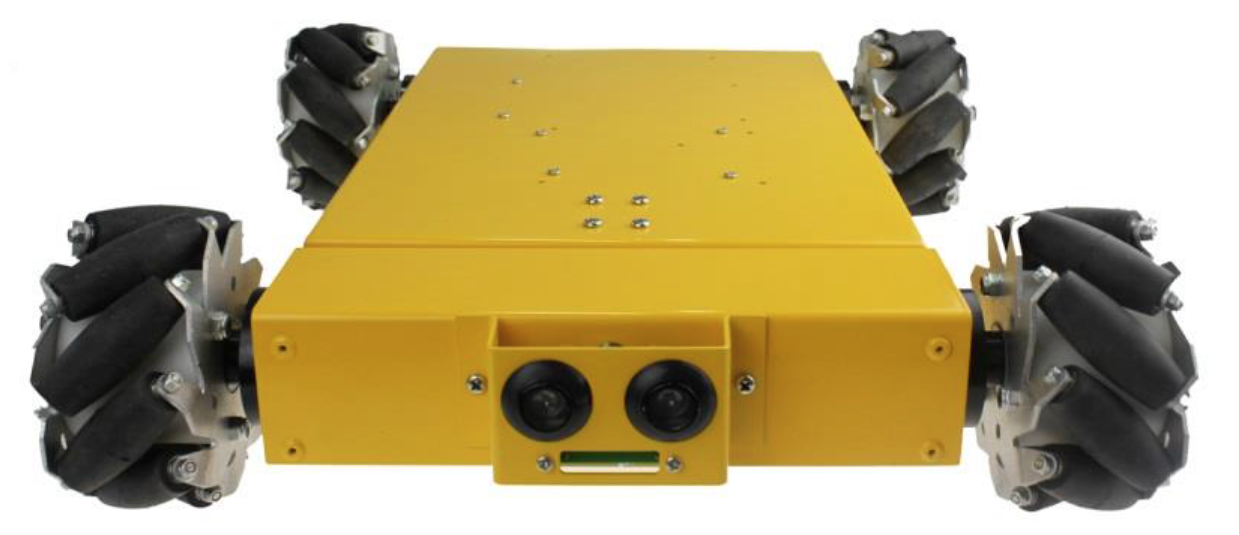
\includegraphics[height=3cm]{figures/mecanum}
	\caption{Mecanum AB robot}
	\label{mecanum}
	\endminipage\hfill
\end{figure} \\
When all four wheels spin in the same direction, the robot moves longitudinally in a straight line forward or backward, accordingly. When one diagonal pair of wheels spin in the same direction and the other diagonal pair of wheels spin in the opposite direction, the robot moves purely laterally. The simultaneous spin can be achieved if the wheels on left side are driven in forward or backward while the wheels on the other side are driven the corresponding opposite direction. As it was discussed earlier, this four-wheel arrangement is not minimal in terms of control, stability and maneuverability, but prefered over three-wheeled configuration for higher capacity and stability reasons. \\[10pt]
Main disadvantages of omnidirectional configurations includes the complexity of control because of the more complex processing of wheel velocities. For instance, the Swedish wheels has a set of free rollers along the wheel perimeter adding extra degrees of freedom,i.e. translation in the lateral direction. Furthermore, due to these rollers the wheel perimeter is not a perfect circle, thus accuracy of dead-reckoning based on counting the number of rotations might be inaccurate soon. The rollers can also cause slippage, thus accumulation of displacement errors.

\paragraph{Anholonomic robots}
The non holonomic wheeled robot configurations are more widely spreaded, e.g. automatic wheelcairs, robot cars. The most common choice of indoor robotics is the well-known two-wheel differential drive due to its simplicity beside acceptable maneuverability, only slightly inferior to omnidirectional drives. In optimal configuration the two wheels are arranged symmetrically, thus the robot can spin around the center point of the case without changing its location. One or two additional ground points, e.g. non driven castor wheel(s), are usually added to gain stability. 
\begin{figure}[htb!]
	\centering
	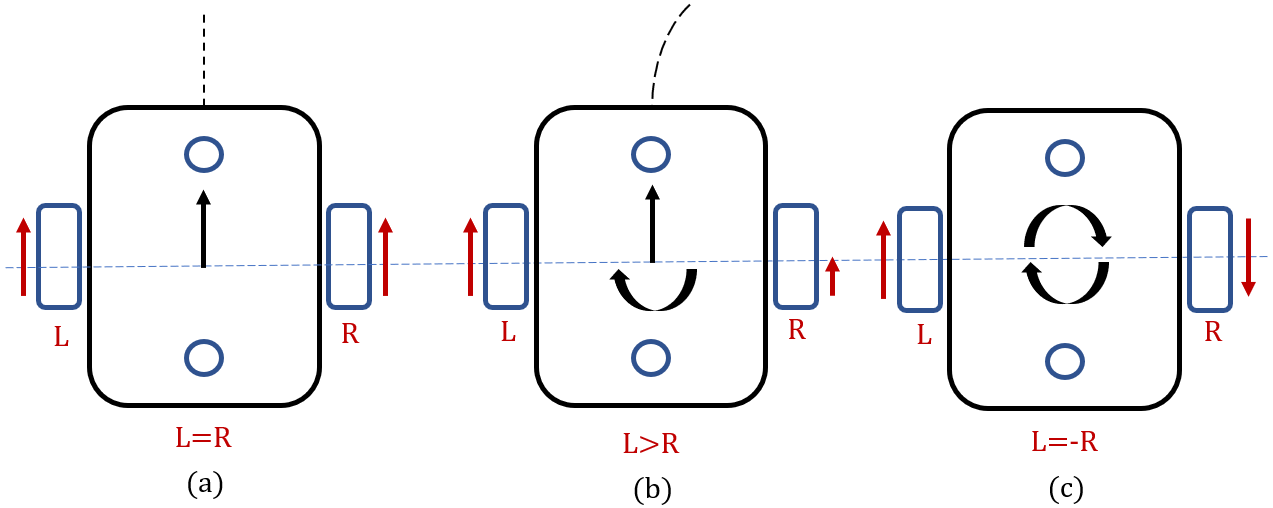
\includegraphics[width=10cm]{figures/differential.png}
	\caption{Two-wheeled differential drive configuration}
	\label{differential}
\end{figure}
In such robotics, motion in a particular direction may initially require a rotational motion to be able to change the position along straight movements. Two wheel differential drive is not clearly omnidirectional but motion can be decomposed 
into distinct rotation and displacement according to the given order. One can say, that it has two and a half degrees of freedom compared to three wheeled omnidirectional configurations that have three whole degrees of freedom.
The advantages includes easy maneuverability, simple construction as only two motors and two conventional wheels needed. Also two wheels can be enough, but in this case self-balancing control has to be attached, in general castor wheels are preferred. The disadvantages of this configuration are lower lateral stability at higher speed turns, sensitivity to terrain roughness, furthermore if the axes of the two wheels are not coincident, the sliding of the wheels will occur.

Similarly to automobiles, remarkable part of the four-wheel robots use the Ackerman steering geometry. It is a way of geometric arrangement of linkages in the steering of a vehicle designed such a way that the inner and outer wheel of a turn can move along circles of different curvatures. 
\begin{figure}[htb!]
	\centering
	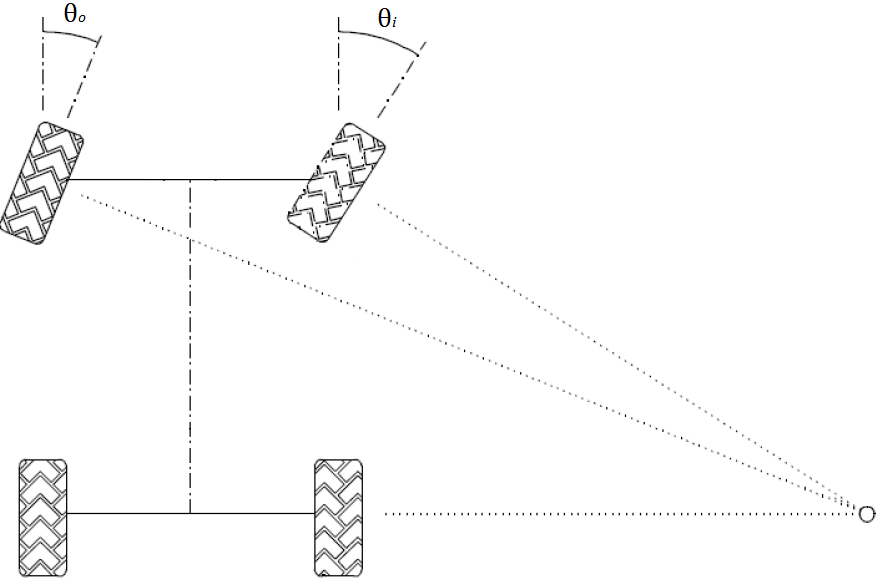
\includegraphics[height=6cm]{figures/ackerman2.png}
	\caption{Ackerman steering arrangement}
	\label{ackerman2}
\end{figure}
It is important that ${\theta}_i$ and ${\theta}_o$ angles cannot be the same whereas in that case the constant sliding of the wheels would be inevitable. In addition, the rear wheels also have to be tuned to spin with different appropriate velocities as they move along different trajectories. As Figure \ref{ackerman2} depicts, such a vehicle typically has a turning diameter that is larger than itself, thus to move sideways requires a parking maneuver consisting of repeated changes in direction forward and backward. In addition, the limited maneuverability of Ackerman steering has an important advantage, i.e. its directionality and steering geometry provide a
very good lateral stability in high-speed turns. Furthermore, it is much more easier to straight simply by locking the steerable wheels and driving the drive wheels compared to the omnidirectional configurations where permanent control is needed.

Multi-degree-of-freedom robots have more than the needed three degrees of freedom. They have enhanced maneuverability, but as a result of the over determined arrangement the slippage free control is more challenging at the same time. The main application scope are mostly the navigation on uneven terrains, e.g. military applications or moon rovers. The position tracking is impossible by odometry, thus external sensors are essentially needed. 

\begin{figure}[htb!]
	\centering
	\minipage{0.5\textwidth}
	\centering
	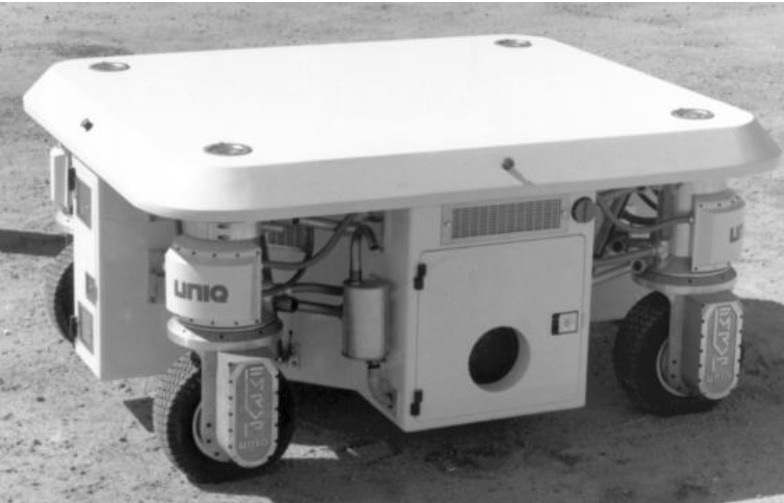
\includegraphics[height=5cm]{figures/uniq.png}
	\caption{UNIQ: 8 DOF mobile robot}
	\endminipage\hfill
	\minipage{0.5\textwidth}
	\centering
	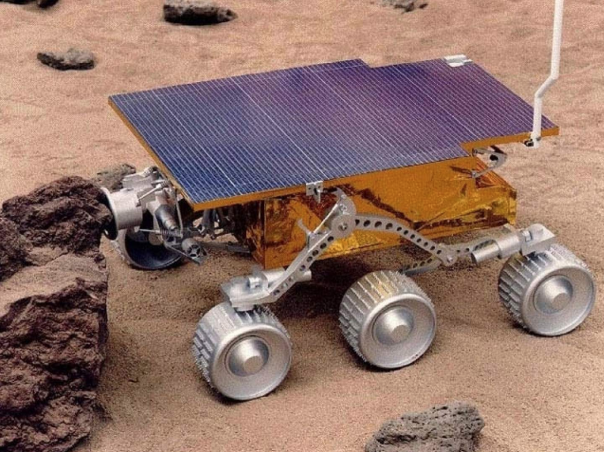
\includegraphics[height=5cm]{figures/rover.png}
	\caption{Sojourner: Mars rover of NASA}
	\label{mecanum}
	\endminipage\hfill
\end{figure}

\newpage
\section{Conditions of the robot application }
\subsection{Selecting a mobile robot configuration}
In previous chapters the basic features of mobile robots and some real life application were presented. This final project basically aims at designing an autonomous transport robot to investigate its control and possible parameter estimation problems. Real world transport robots are usually capable to navigate along prescribed path, monitor their environment to handle unexpected obstacles, interact with the packages autonomously and communicate with users surrounding them. These are the most necessary features that are really needed during operation which have been mostly implemented in the past.

The development of kinematic and dynamic properties have been taken less attention so far, therefore this field can contain remarkable development potential in my opinion. The transport robots in industrial application are designed such a way that during their movement they will not likely face issues regarding the stability because they move along
high radius path with low speed and accelerate moderately. In other words, a compromise is made between the configuration costs and the productivity, between the security and effectiveness. Sooner or later, the demand for a more dynamic, faster and smoother operation of transport robots can come into being just like in automotive industry. The problem can be more complex as well in certain situations. For instance, a transport robot operating in a plant that carries loads with different properties such as mass, moment of inertia or height would face a more challenging situation in dynamic stability point of view than a car with more or less known and constant physical parameters.

To select a mobile configuration, the general purpose, working environment and concept of the robot have to be defined. Based on real life experience and possible future application needs, this study will focus on designing a transport robot which would operate in a plant, in a laboratory or on the streets carrying different shaped and weighted loads. Instead focusing on navigation, i.e. dead-reckoning, route planning and obstacle avoiding, the control of dynamic behaviour is to be examined in details. Beside the technological aspects also the practibality and costs have to be considered because the building of the mobile robot configuration is also the part of my thesis. The most important aspect of a study of such a advanced moving transport robot is the maneuverability. In terms of maneuverability, the omnidirectional robots show the best performance. Choosing a three-wheeled omnidirectional mobile robot configuration can be regarded the optimal choice. The controllability is more complex compared to anholonomic robots, but with the choice of minimum number of three wheels it is still a handleable design challenge. Application of more wheels could give more controllability which would be favoured, e.g. TUG is also four wheel driven omnidirectional configuration. However, it would make some additional issues appear such increased slip danger and more complex controllability. Compared to anholomic configuration, the holonomic configurations are less stable as mentioned before, but it can be regarded as an advantage in this case, because this study is willing to deal with stability issues, thus the main objective is to examine the behaviour of the system near stability and provide parameter estimation methods to avoid it.
In other words, a transport robot might be preferred over others if it can be as stable as possible without loosing any maneuverability skill. For an omnidirectional drive configuration special wheels of higher price are need, thus the three-wheeled configuration is optimal from economic point of view.
\newpage
\subsection{The Hardware}
\subsubsection{Robot case and actuators}
\subsubsection{MCU}
\subsubsection{Sensors, modules and battery}
\subsubsection{Assembly}

\newpage
\subsection{Kinematics of three-wheeled omnidirectional robot}
\subsubsection{Basic relationships}
Let us define the global frame as [X,Y] coordinate system which represent the environment. The location and the orientation of the robot can be described with (X,Y,$\alpha$) or (X,Y,$\varphi$) vector, while the kinematic state as that of time-derivative, i.e. ($\dot X, \dot Y, \dot \alpha$) or ($\dot X, \dot Y, \dot \varphi$). Eventually, we are usually interested in the kinematics from global frame point of view, but from the design and user point of view it is more convenient to start writing the equations in the local frame of the robot and then transform the kinematics to the global frame if that is needed. Let us denote the local frame as $(x,y)$ which center is the center of gravity of the robot. The robot velocity as $v$ when that of components in the local frame are $(v_x,v_y) = (- v sin \gamma , v cos \gamma )$.

\begin{figure}[htb!]
	\centering
	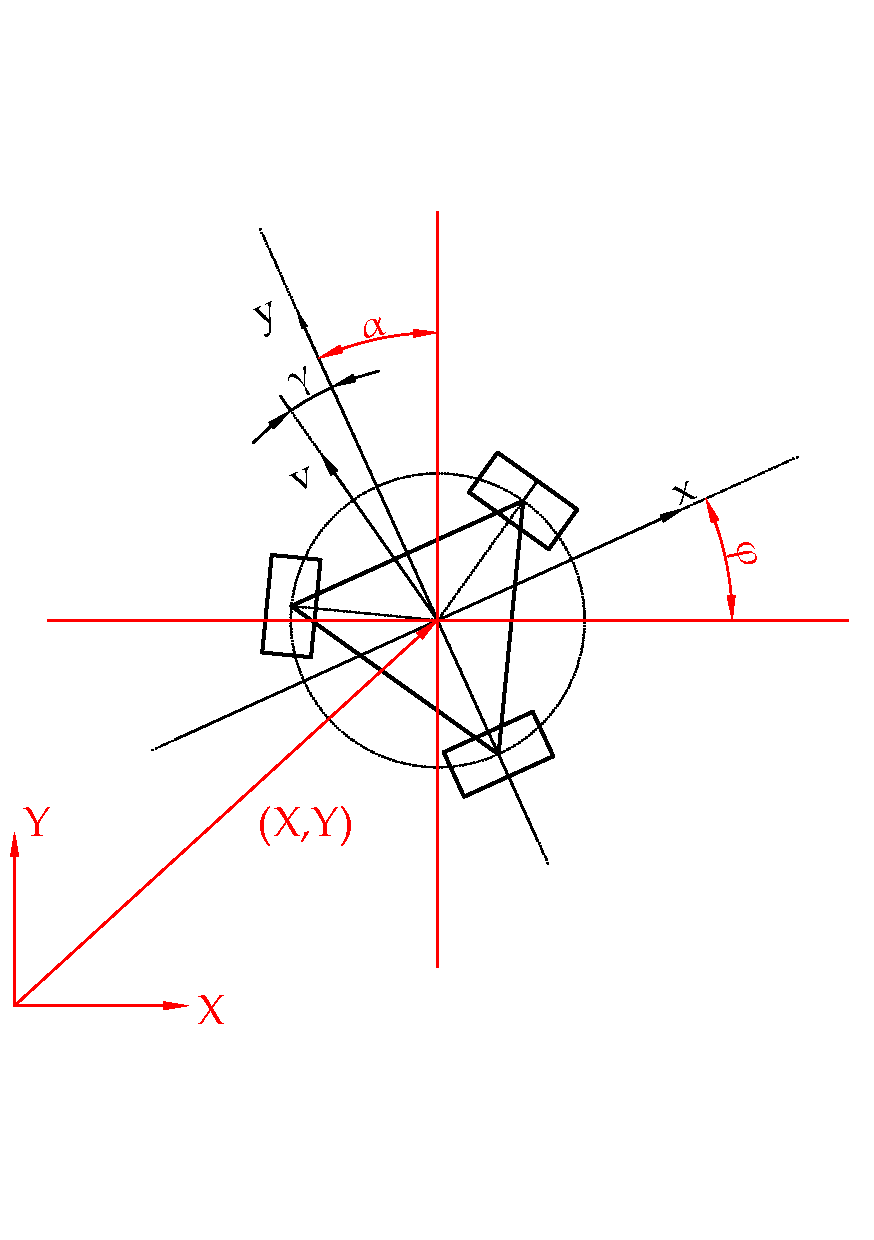
\includegraphics[width=7cm]{figures/global_local_frame}
	\caption{Global and local frames of the robot}
	\label{global_local_frame}
\end{figure}
The overall kinematic state of the case is a straightforward resultant of the wheel kinematic states. The velocity of wheels can have two type of components:
\begin{itemize}
	\item Translational velocity which actually equals with translational speed of the case because of the kinematic constraint. Additionally, it can be divided into two further parts:
		\begin{itemize}
			\item Its own velocity which can be called as pure translational wheel speed. It is proportional with the angular velocity of the wheel $v_{wheel,t} ~ r \omega_i$, where r is the wheel radius and $\omega$ is the angular velocity.
			\item The rolling velocity $v_{roller}$ which is induced by the other wheels and realized by the free rollers. Its direction is determined by the construction of rollers, generally and also in this case let it assume to be 90$^{\circ}$.
		\end{itemize}
	\item Rotational velocity component which comes from the spinning of the whole robot case about its center of gravity which can be supposed to be in the geometrical center of the common wheel circle, therefore it can be formulated as $v_{wheel,r}  = R \dot \alpha$. This component is always the same for all wheels.
\end{itemize}
The resultant translational wheel velocity can be calculated as:
\begin{equation}
v^i = {v_{wheel,t}}^i + {v_{wheel,r}} = r \omega_i
\end{equation}
where $i$ is the index of the wheels and i=1,2,3 in case of a thee-wheeled omnidirectional robot.
\begin{figure}[htb!]
	\centering
	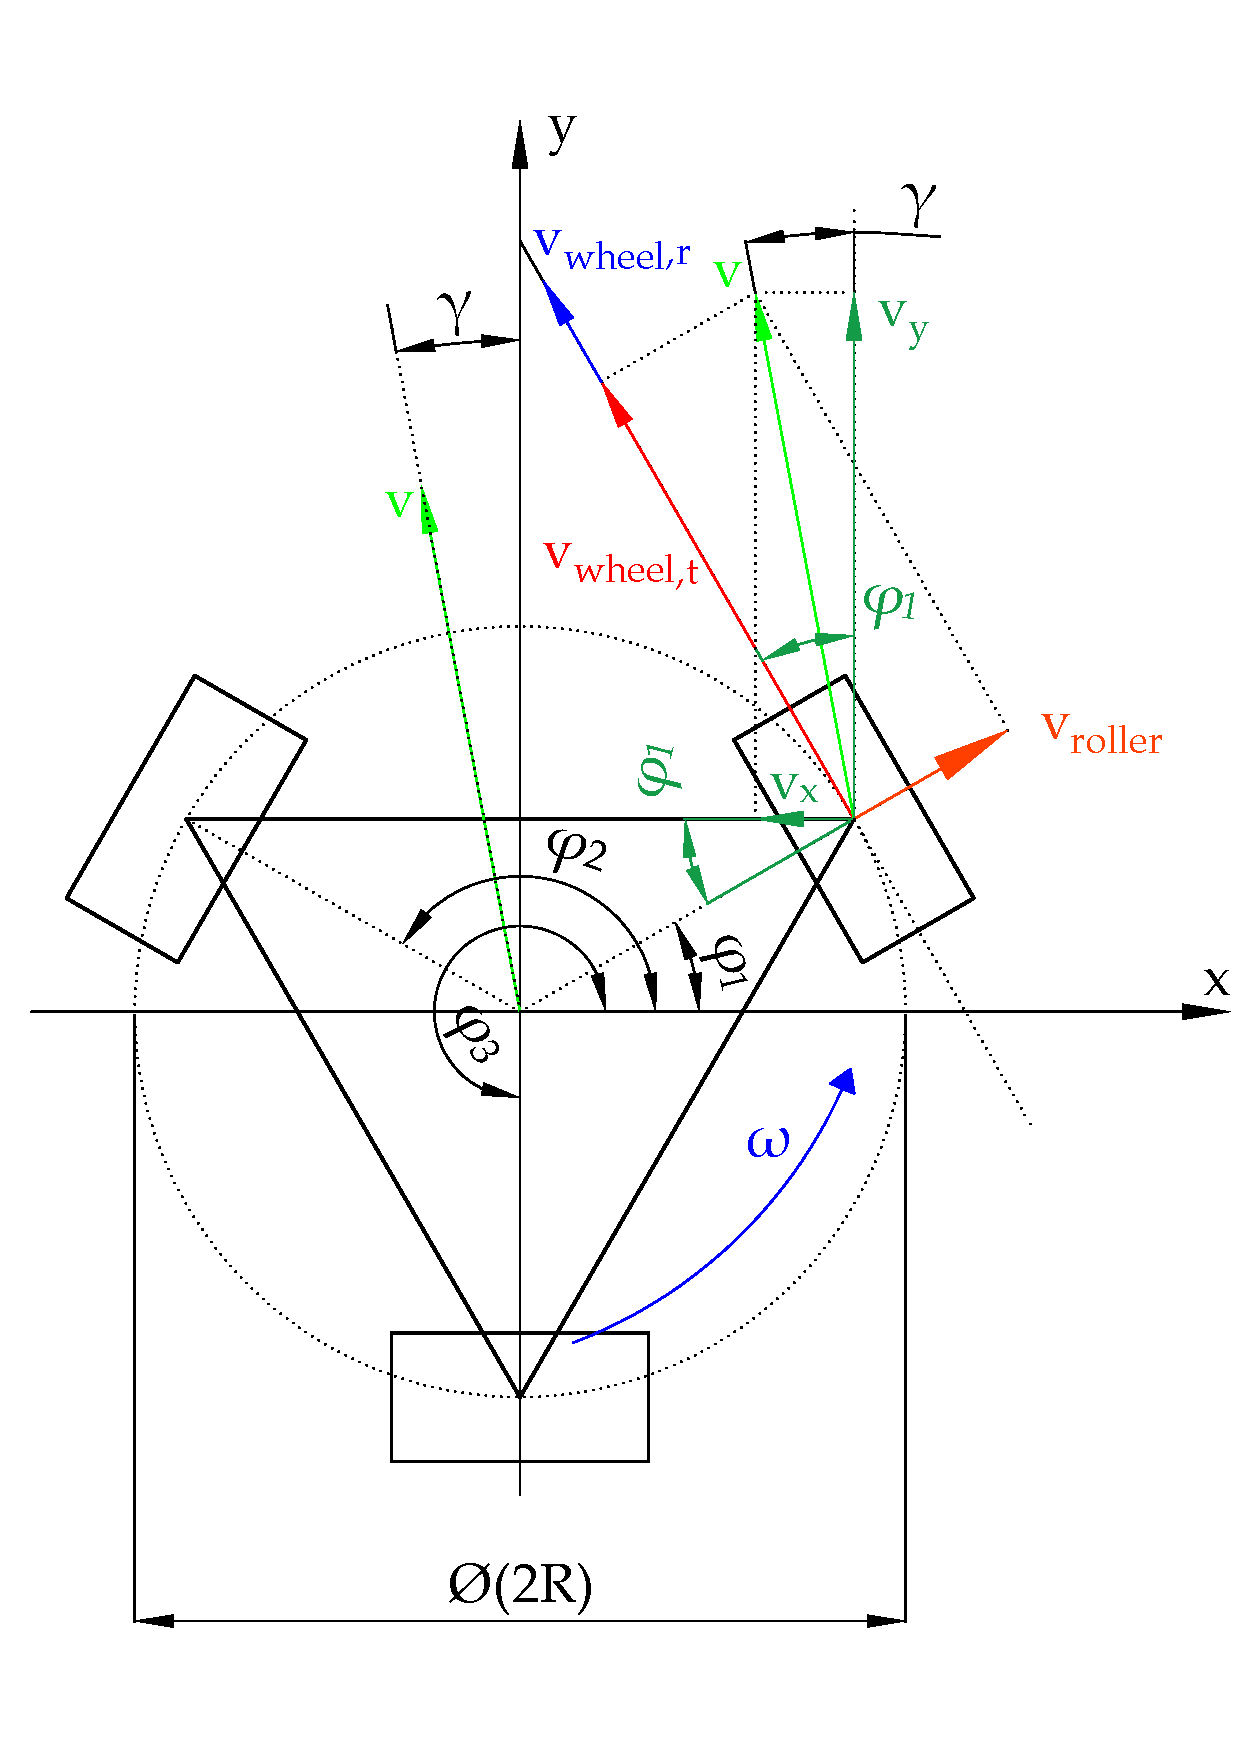
\includegraphics[width=10cm]{figures/omni_wheel_vectors}
	\caption{Wheel vectors in local (x,y) coordinate system}
	\label{omni_wheel_vectors}
\end{figure}

The omniwheels are located along the common wheel circle (R) at $\varphi_1, \varphi_2, \varphi_3$ angles measured from the local $x$ axis. The pure translational part of the wheel velocity can be written as a combination of the x,y components of the robot translational velocity as:
\begin{equation}
	{v_{wheel,t}}^i = - v_x sin \varphi_i  + v_y cos \varphi_i .
\end{equation}
Considering the equations above the total wheel velocity is:
\begin{equation}
	v_i = - v_x sin \varphi_i + v_y cos \varphi_i  + R \omega_i,
\end{equation}
therefore the angular velocity of the wheel is:
\begin{equation}
	\omega_i = \frac{1}{r} (- v_x sin \varphi_i + v_y cos \varphi_i + R \omega_i),
\end{equation}
which can be generalized in vectorial form as:
\begin{equation}
	\boldsymbol{\omega} = \mathbf{J^{-1}} \mathbf{v}
\end{equation}
where
\begin{itemize}
	\item $\Omega = [\omega_1~\omega_2~\omega_3]^T$ is the wheel angular velocity vector,
	\item $\mathbf{J^{-1}}$ is the inverse Jacobian matrix of the case velocities which is
		\begin{eqnarray}
		\mathbf{J^{-1}}=\frac{1}{r} \left[
		\begin{array}{ccc}
		sin \varphi_1 & cos \varphi_1 & R \\
		sin \varphi_2 & cos \varphi_2 & R \\
		sin \varphi_3 & cos \varphi_3 & R \\
		\end{array}
		\right],
		\end{eqnarray}
	\item $\mathbf{v} = [v_x~v_y~\omega]^T = [\dot x~\dot y~\dot \varphi]^T$ is the case velocity vector.
\end{itemize}
The inverse of determinant of J is never zero, thus its inverse always exists which means that kinematic relation between the wheels and the case is provided. In order to track the robot in the global configuration, the kinematic state has to be transformed from the local frame to the global frame which can be done by means of a simple rotation transformation perpendicular to (x,y) plane with $\alpha$ orientation angle:
\begin{equation}
\boldsymbol{x} = \mathbf{T}~\mathbf{X}
\end{equation}, i.e.
\begin{eqnarray}
\left[
\begin{array}{c}
\dot x \\
\dot y 	\\
\dot \phi \\
\end{array}
\right]=
\left[
\begin{array}{ccc}
cos \alpha 	& -sin \alpha & 0 \\
sin \alpha 	& cos \alpha & 0 \\
0	 		& 0 		 & 1 \\
\end{array}
\right]
\left[
\begin{array}{c}
\dot X \\
\dot Y 	\\
\dot \Phi \\
\end{array}
\right].
\end{eqnarray}
\subsubsection{2D Simulations}
Considering the equations above, a two-dimensional kinematic simulator was built-in Mathematica which could help to understand more accurately the robot locomotion mechanism by calculating and then visualizing the movements. The simulator has to be initialized with as follows:
\begin{itemize}
	\item Common wheel circle (R) which is in this case: caseR = 0.12 m,
	\item Wheel position angles ($\varphi_i$) which is in this case $\varphi_1=30^{\circ}, \varphi_1=150^{\circ},\varphi_1=270^{\circ}$,
	\item Initial position and orientation $\mathbf{X} = [X~Y~\alpha]^T$, i.e. $\mathbf{p}=[X~Y]^T$ and $\alpha$,
	\item Initial velocity state in the local frame: $\mathbf{v} = [v_x~v_y~\omega]^T,$ i.e. $v,~\gamma$ and $\omega$.
	\item The solution is obtained numerically, integrating the velocities over time steps, thus timestep size ($dt$ )and simulation time (T) has to be provided.
\end{itemize}
The basic equations are the followings:
\begin{itemize}
	\item The new position equation is
	\begin{equation}
		\mathbf{p}^{i+1} = \mathbf{p}^{i} + \mathbf{T} \mathbf{v}^i dt,
	\end{equation}
	\item The new orientation equation is
	\begin{equation}
		\alpha^{i+1} = \alpha^{i} + \omega^i dt.
	\end{equation}
	\item The new velocity magnitude equation is
	\begin{equation}
		v^{i+1} = F(v^{i},dt,\mathbf{p}^{i},...).
	\end{equation}
	\item The new velocity direction equation is
	\begin{equation}
		\gamma^{i+1} = F(\gamma^{i},dt,\omega,...).
	\end{equation}
	\item The new angluar velocity equation is
	\begin{equation}
	\omega^{i+1} = F(\omega^{i},dt,\mathbf{p}^{i},...).
	\end{equation}
\end{itemize}

The Figure \ref{relation_v_1_g_0_w_0} depict a pure translation in forward direction. An interesting characteristic of the robot configuration can be observed, i.e. the resultant case velocity can be greater than the wheel velocities. The Figure \ref{relation_v_0_g_0_w_10} represent the case of pure rotation when the wheel velocities are equal.
\begin{figure}[htb!]
	\centering
	\minipage{0.5\textwidth}
	\centering
	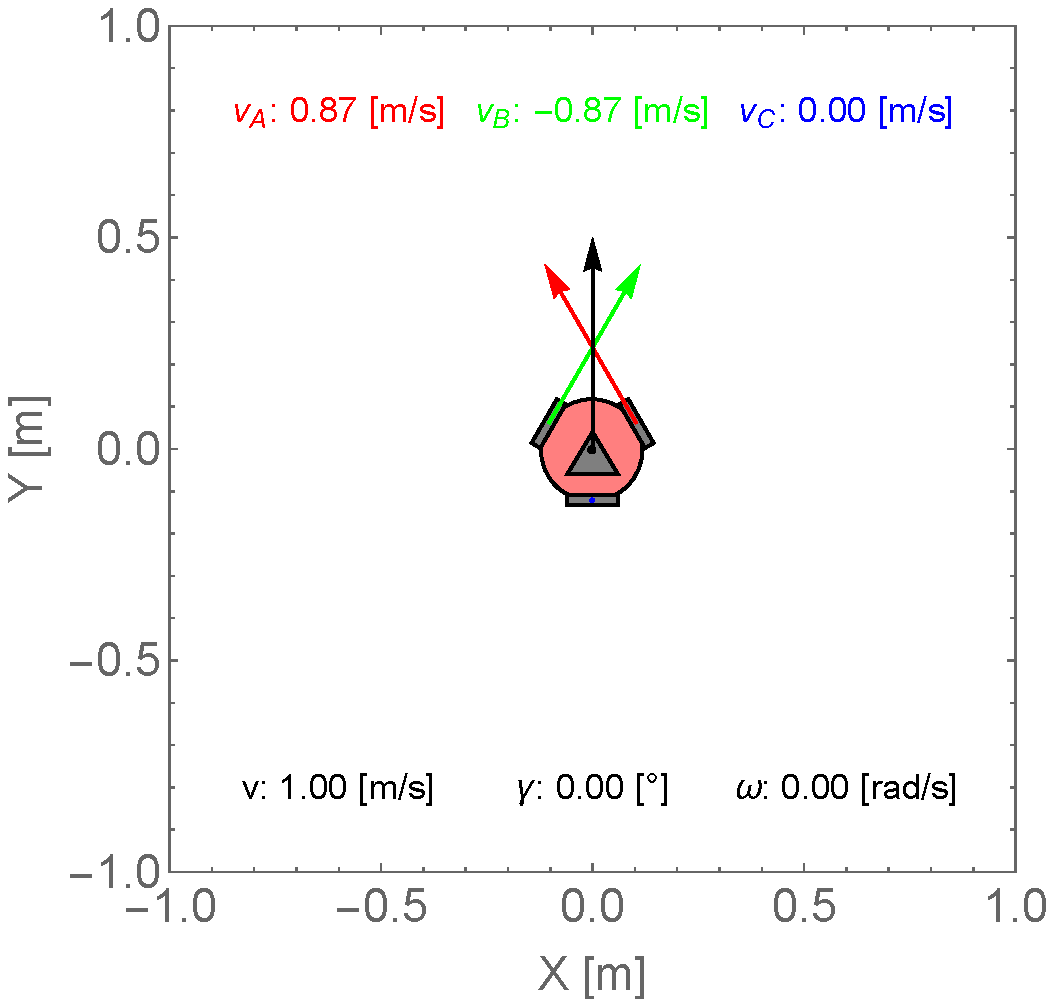
\includegraphics[height=7cm]{figures/2d_simulation/relation_v_1_g_0_w_0}
	\caption{Pure forward translation}
	\label{relation_v_1_g_0_w_0}
	\endminipage\hfill
	\minipage{0.5\textwidth}
	\centering
	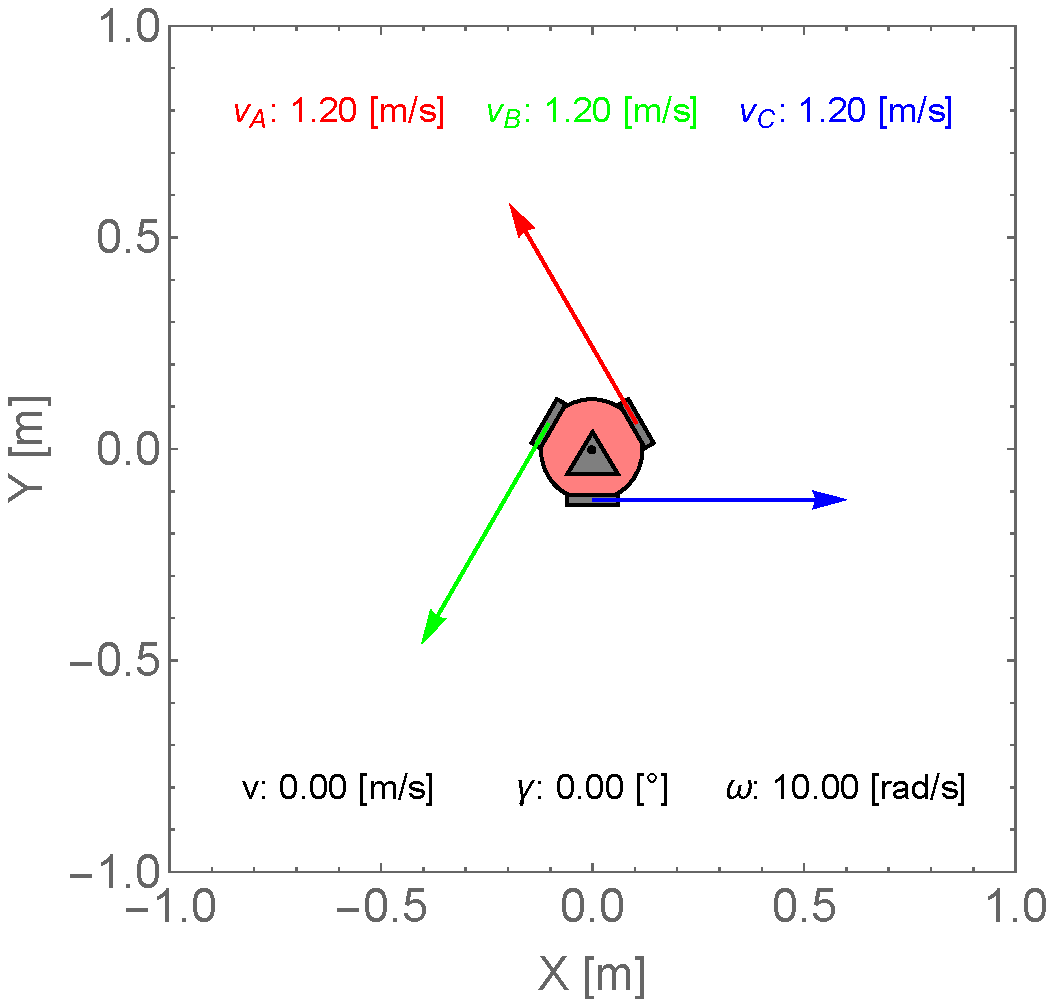
\includegraphics[height=7cm]{figures/2d_simulation/relation_v_0_g_0_w_10}
	\caption{Pure spinning}
	\label{relation_v_0_g_0_w_10}
	\endminipage\hfill
\end{figure}
The Figure \ref{relation_v_1_g_30_w_0} depicts another specific case of pure translation when the velocity of wheel A equals the robot velocity, while the others drive with same speed but the opposite direction. The Figure \ref{relation_v_06_g_45_w_6} represent a mixed case of translation in an arbitrary direction and rotation at the same time.
\begin{figure}[htb!]
	\centering
	\minipage{0.5\textwidth}
	\centering
	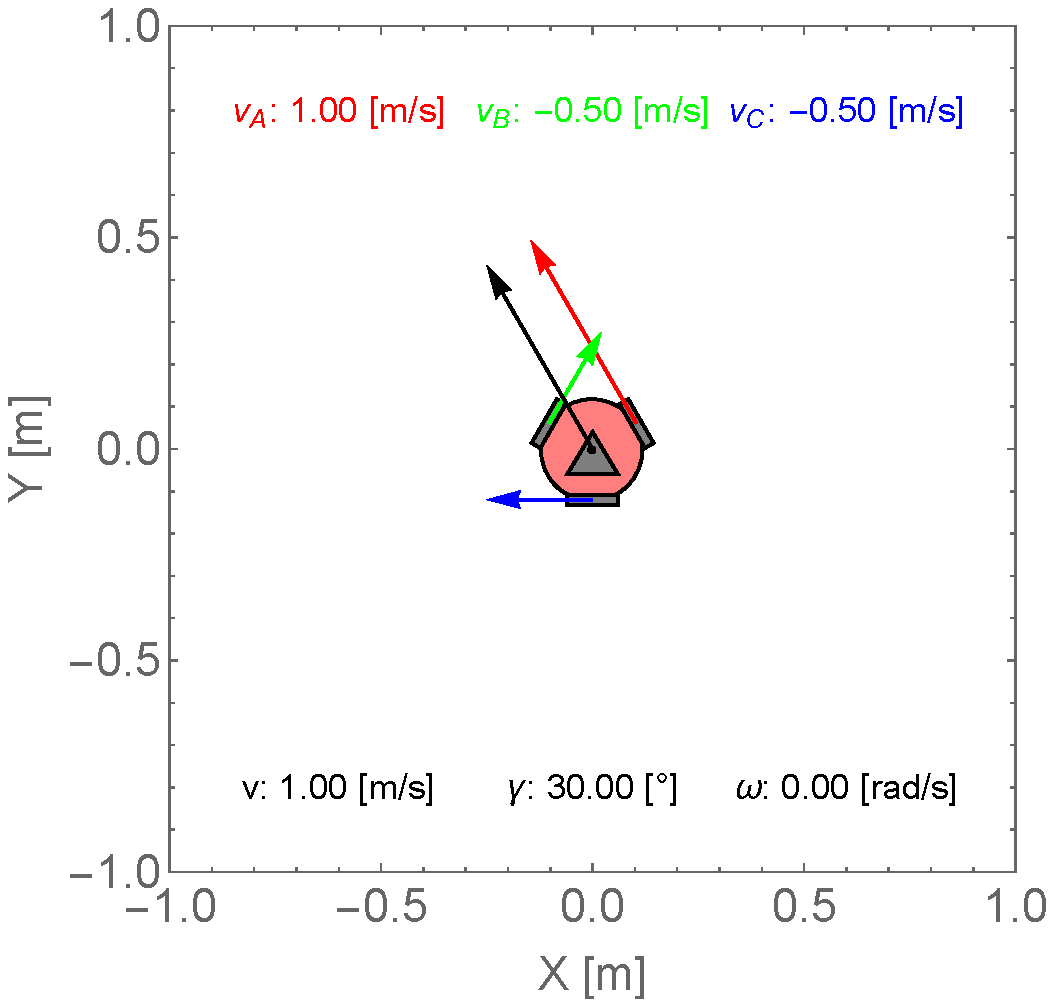
\includegraphics[height=7cm]{figures/2d_simulation/relation_v_1_g_30_w_0}
	\caption{Specific case of translation}
	\label{relation_v_1_g_30_w_0}
	\endminipage\hfill
	\minipage{0.5\textwidth}
	\centering
	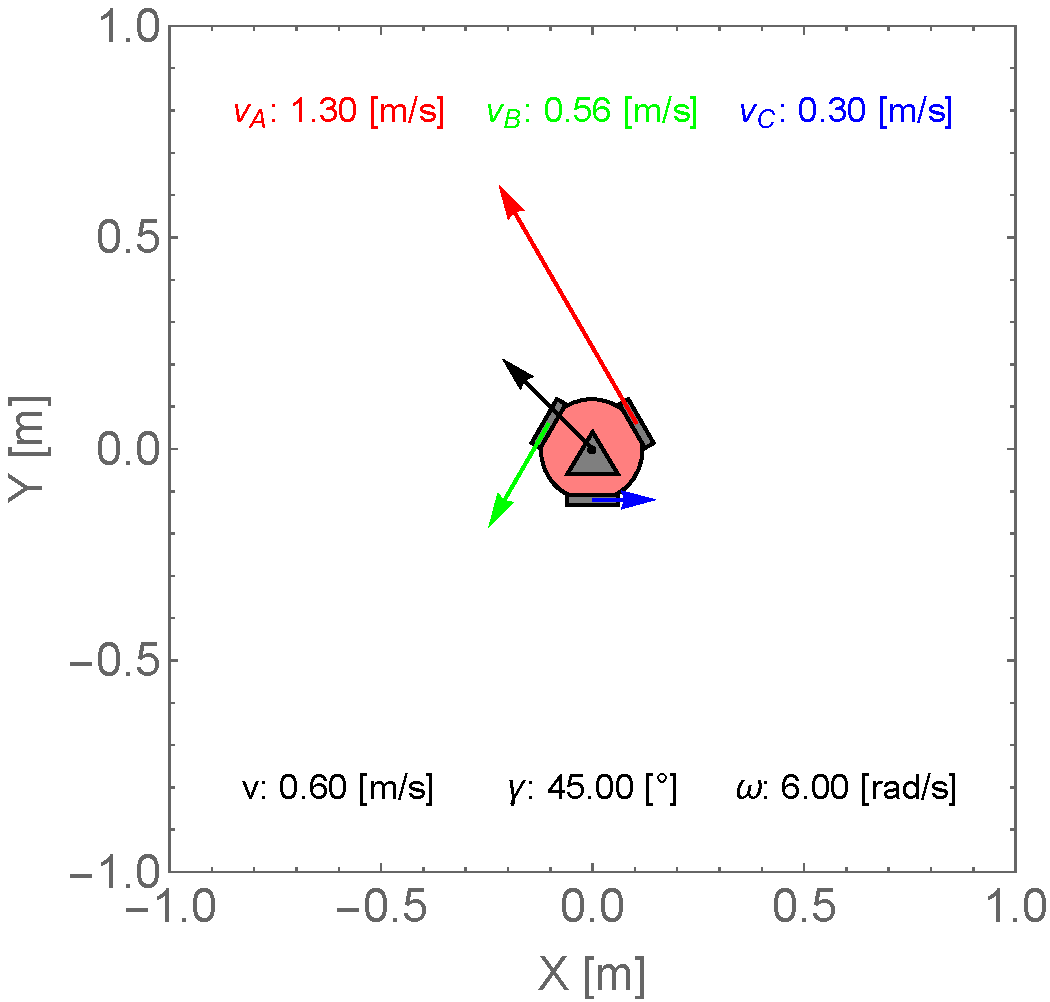
\includegraphics[height=7cm]{figures/2d_simulation/relation_v_06_g_45_w_6}
	\caption{Translation \& rotation}
	\label{relation_v_06_g_45_w_6}
	\endminipage\hfill
\end{figure}
\newpage
The following figures represent the status of robots at given time steps during the simulations. The main equations that generates the shown motions are given. Generally there are 3 parameters to vary: the magnitude of the speed, the direction of the speed and the angular velocity.\\[0.3cm]
\noindent Moving along a circle without changing the orientation:
\begin{itemize}
	\item $dt=0.1~[\text{s}]$ (timestep size), $T=10~[\text{s}]$ (simulation time),
	\item $v^{i+1} = v^{i} = v^{0}$ (constant speed),
	\item $\omega^{i+1} = \omega^{i} = 0$ (no angular velocity),
	\item $\gamma^{i+1} = \gamma^i + \dot \gamma dt$ where $\dot \gamma = \frac{2 \pi}{T}$
\end{itemize}
\begin{figure}[htb!]
	\minipage{0.33\textwidth}
	\centering
	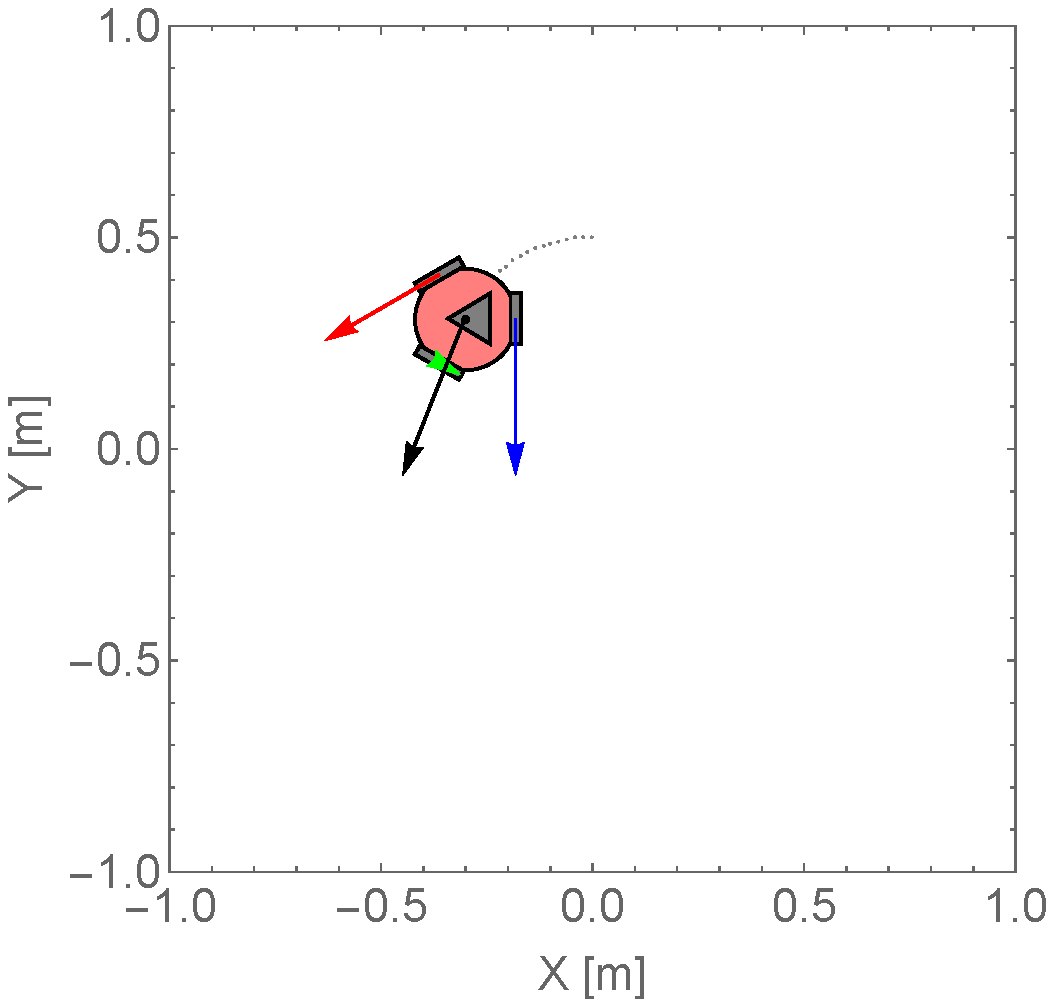
\includegraphics[height=5cm]{figures/2d_simulation/animations/2D_move_along_circle_not_rotating/20}
	\caption{$0.20[s]$}
	\endminipage\hfill
	\minipage{0.33\textwidth}
	\centering
	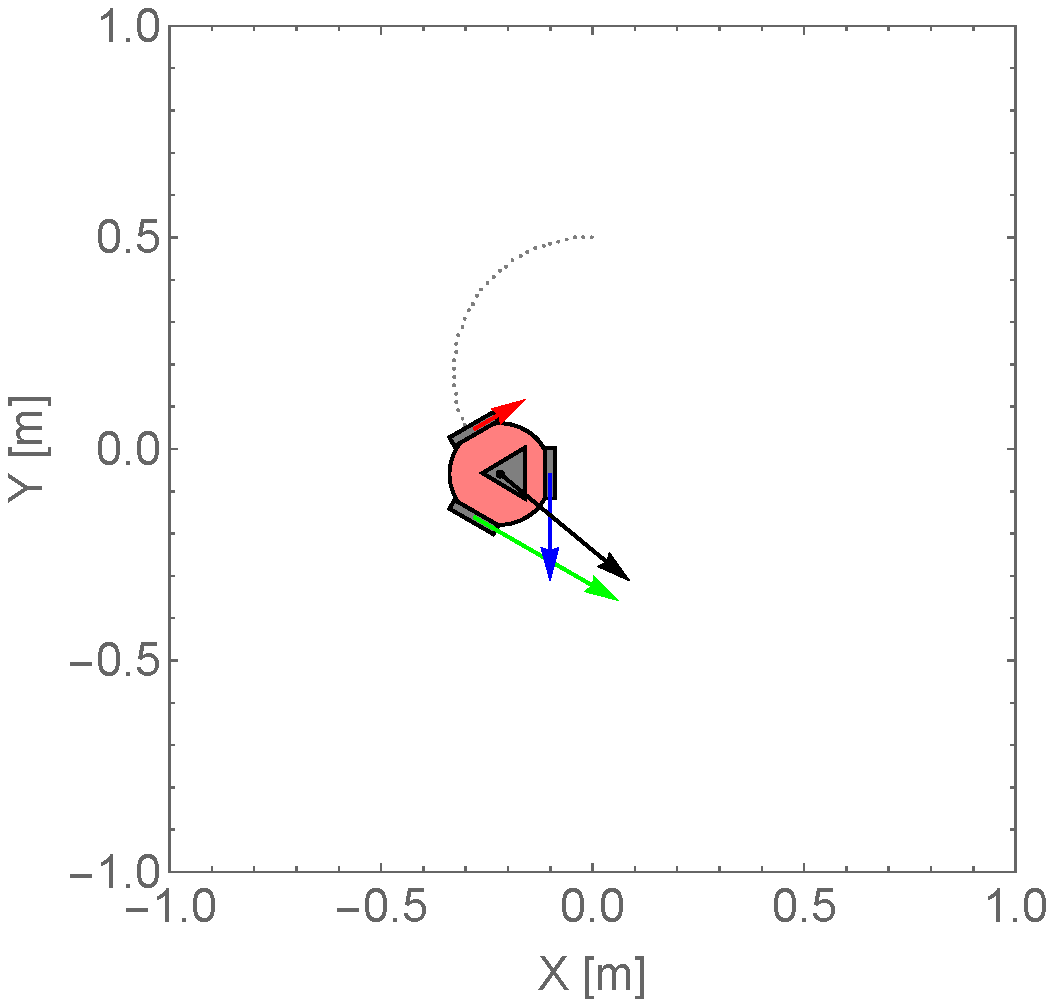
\includegraphics[height=5cm]{figures/2d_simulation/animations/2D_move_along_circle_not_rotating/40}
	\caption{$0.40[s]$}
	\endminipage\hfill
	\minipage{0.33\textwidth}
	\centering
	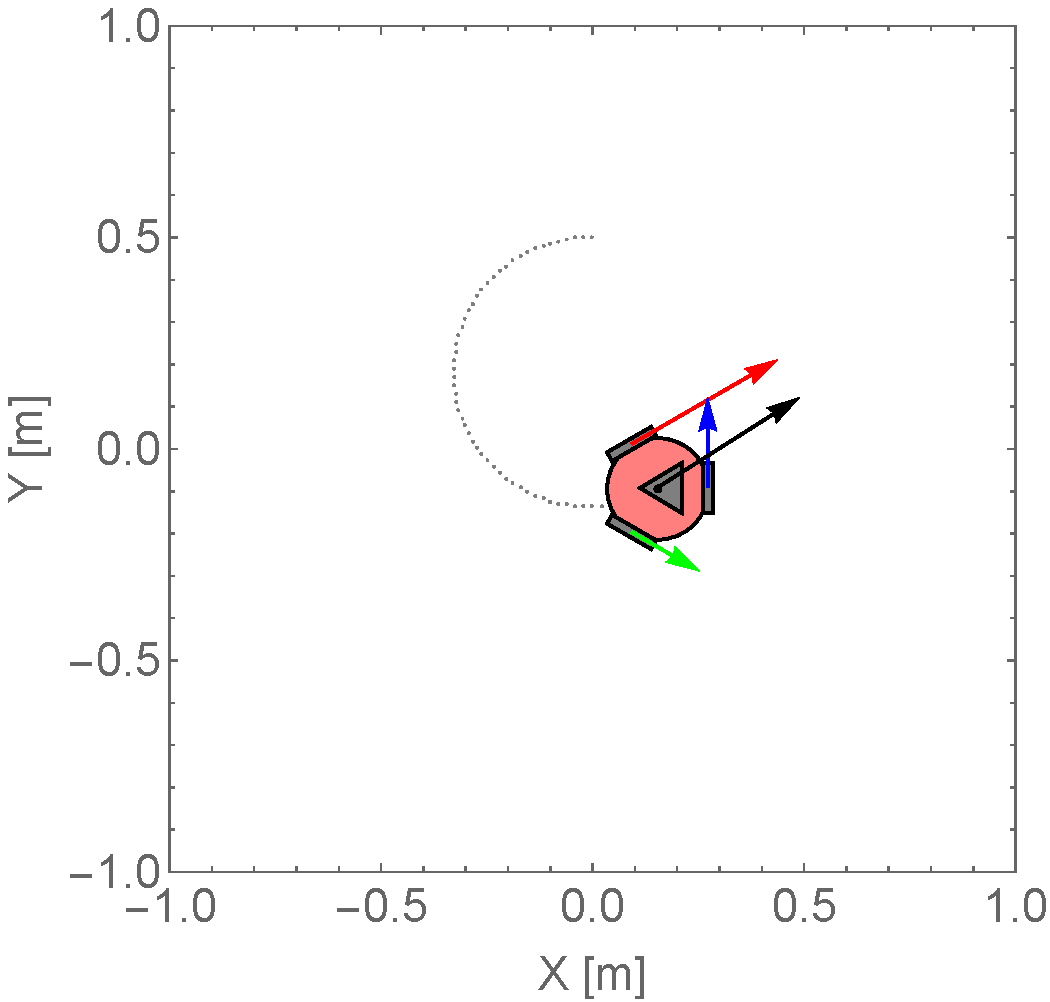
\includegraphics[height=5cm]{figures/2d_simulation/animations/2D_move_along_circle_not_rotating/60}
	\caption{$0.60[s]$}
	\endminipage\hfill
\end{figure}
The direction of the speed vector ($\gamma$) is defined in the local coordinate system and it has to be changed to make the robot move along a given curve, in this case along a circle.\\[0.3cm]
\noindent Moving along a circle without like a car (anholonomic):
\begin{itemize}
	\item $dt=0.1~[\text{s}]$ (timestep size), $T=10~[\text{s}]$ (simulation time),
	\item $v^{i+1} = v^{i} = v^{0}$ (constant speed),
	\item $\omega^{i+1} = \omega^{i} = \omega^{0}$ (constant angular velocity),
	\item $\gamma^{i+1} = \gamma^i = 0$
\end{itemize}
\begin{figure}[htb!]
	\minipage{0.33\textwidth}
	\centering
	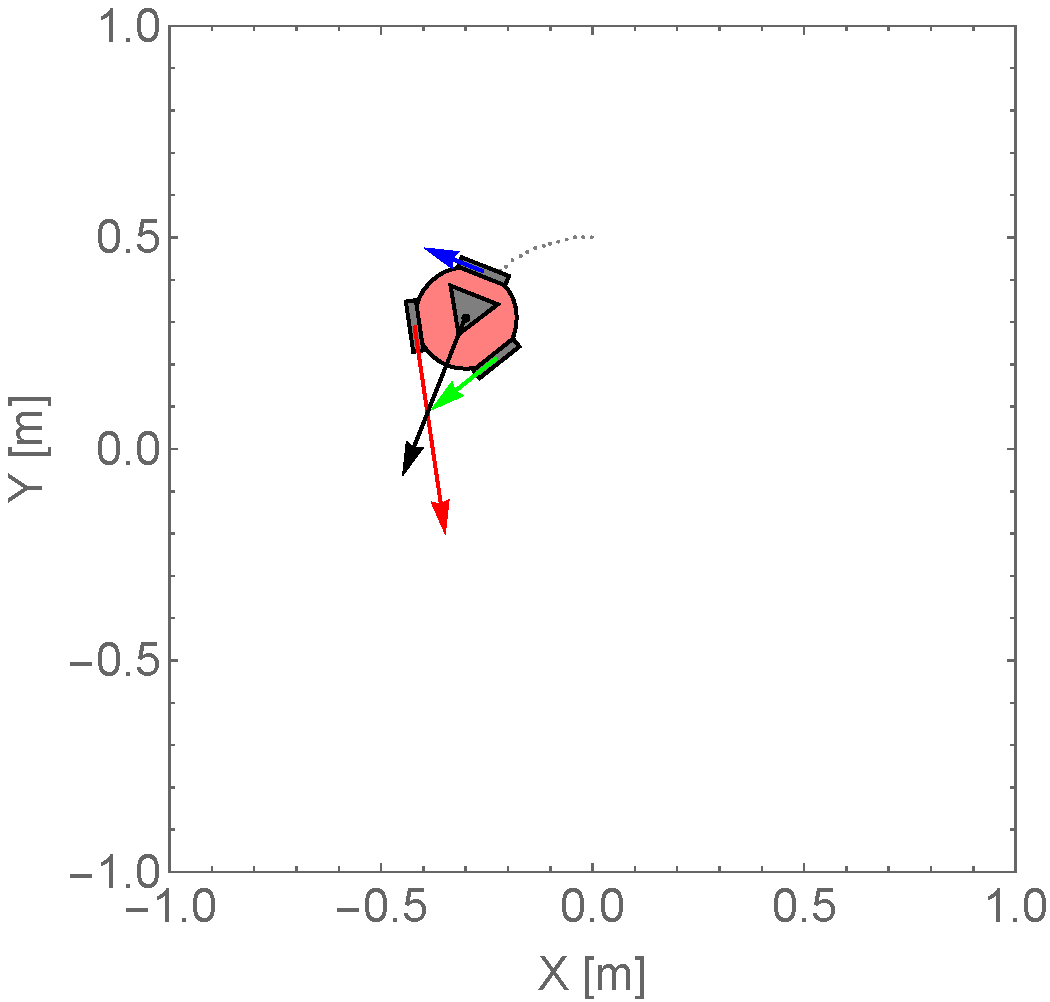
\includegraphics[height=5cm]{figures/2d_simulation/animations/2D_move_along_circle_rotating_car_like/20}
	\caption{$0.20[s]$}
	\endminipage\hfill
	\minipage{0.33\textwidth}
	\centering
	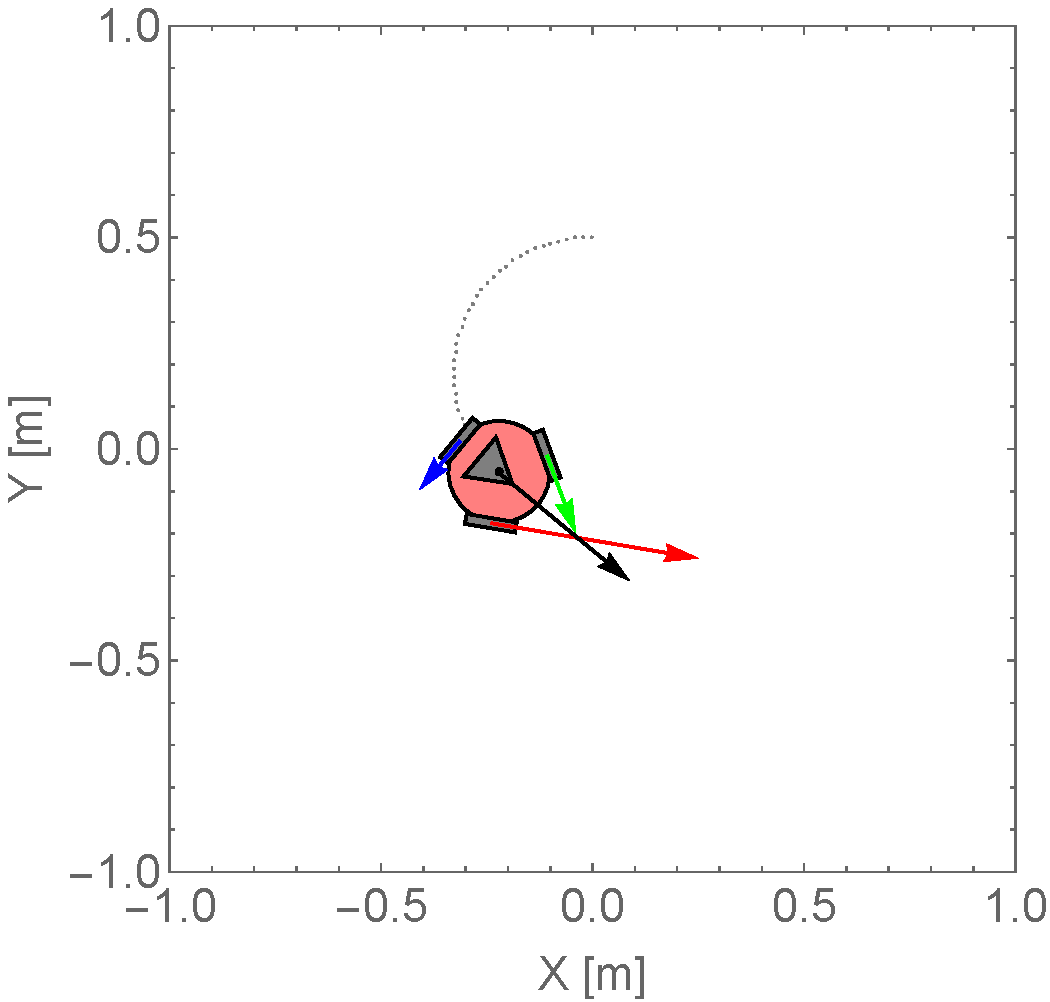
\includegraphics[height=5cm]{figures/2d_simulation/animations/2D_move_along_circle_rotating_car_like/40}
	\caption{$0.40[s]$}
	\endminipage\hfill
	\minipage{0.33\textwidth}
	\centering
	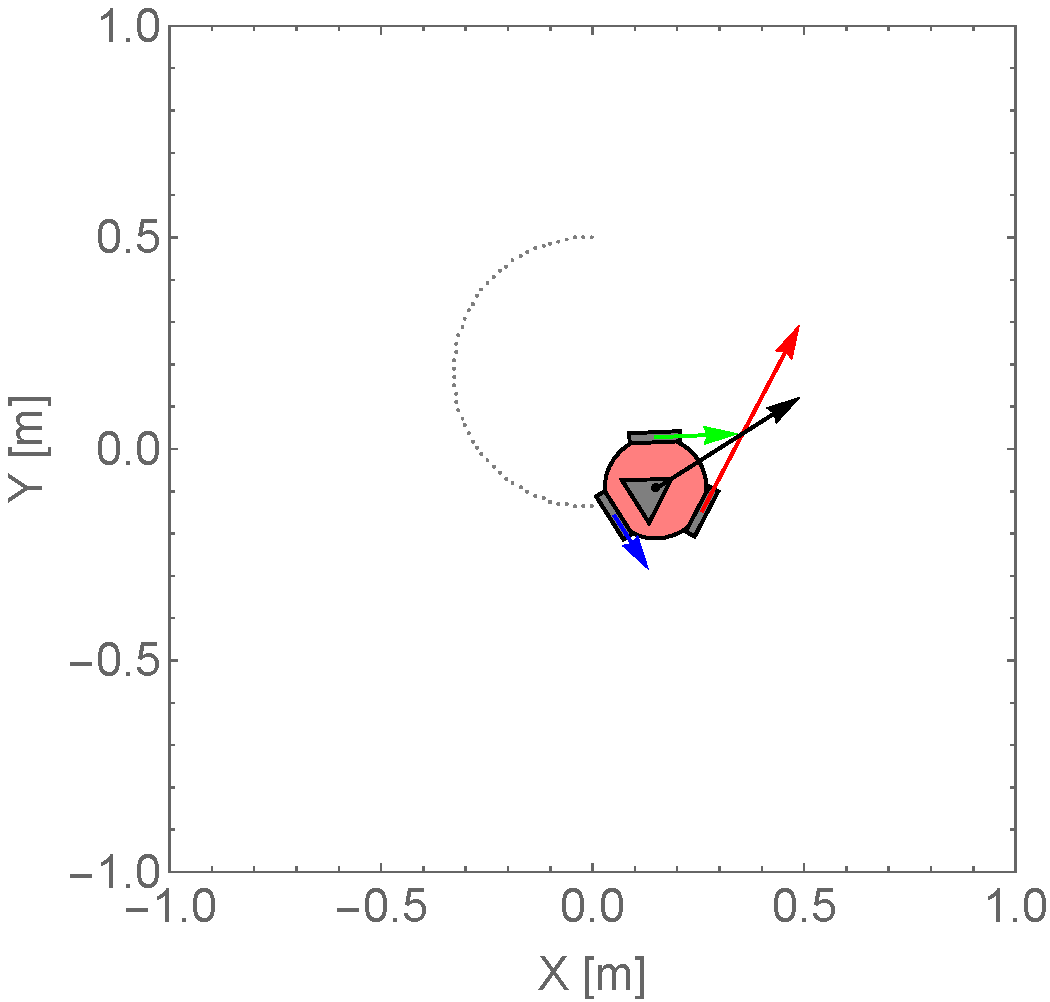
\includegraphics[height=5cm]{figures/2d_simulation/animations/2D_move_along_circle_rotating_car_like/60}
	\caption{$0.60[s]$}
	\endminipage\hfill
\end{figure}
\newpage
The following two cases are further demonstration of the fact that the orientation can be controlled independently from the the orientation, i.e. the robot has 3 DoF. \\[0.3cm]
\noindent Moving along a circle changing the orientation in reverse direction:
\begin{itemize}
	\item $v^{i+1} = v^{i} = v^{0}$ (constant speed),
	\item $\omega^{i+1} = \omega^{i}<0$ (angular velocity),
	\item $\gamma^{i+1} = \gamma^i + \dot \gamma dt -\omega^i dt$ where $\dot \gamma$ is a constant.
\end{itemize}
\begin{figure}[htb!]
	\minipage{0.33\textwidth}
	\centering
	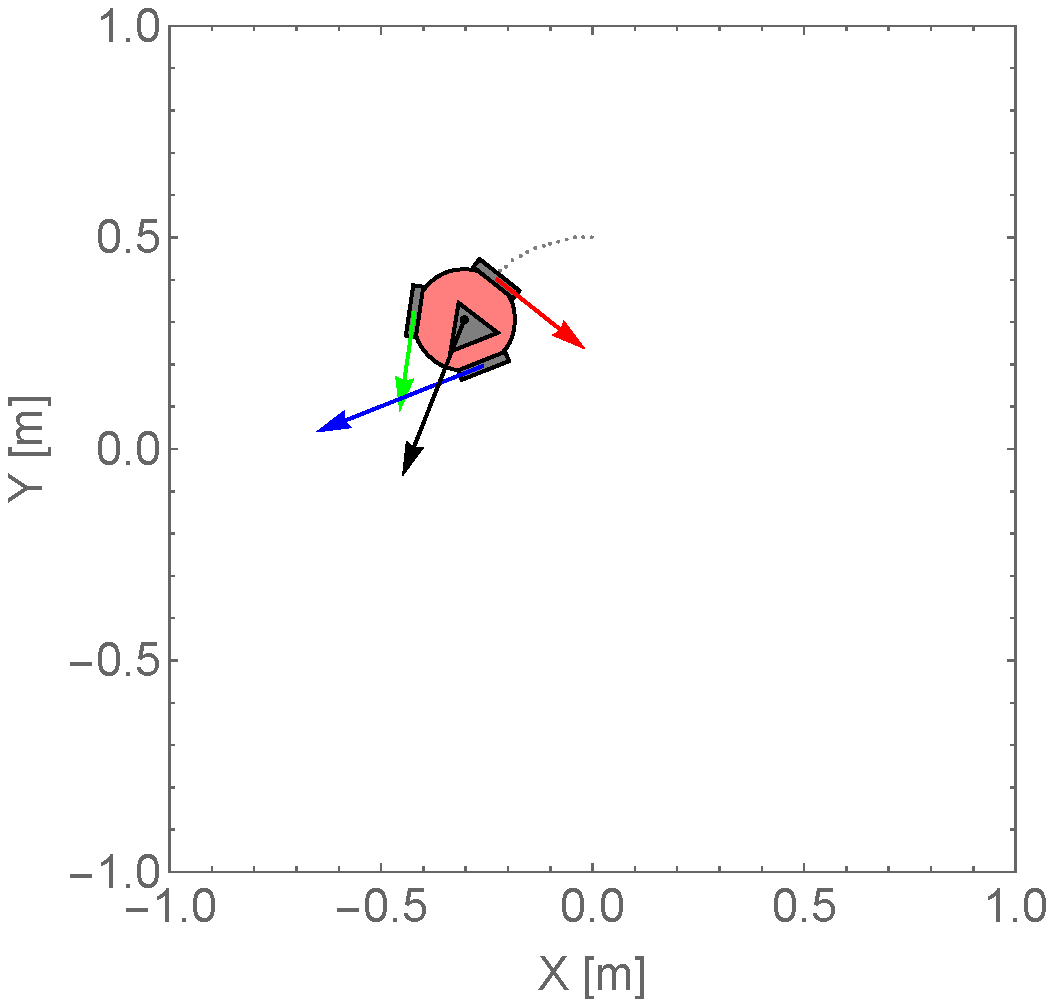
\includegraphics[height=5cm]{figures/2d_simulation/animations/2D_move_along_circle_rotating_reverse_direction/20}
	\caption{$0.20[s]$}
	\endminipage\hfill
	\minipage{0.33\textwidth}
	\centering
	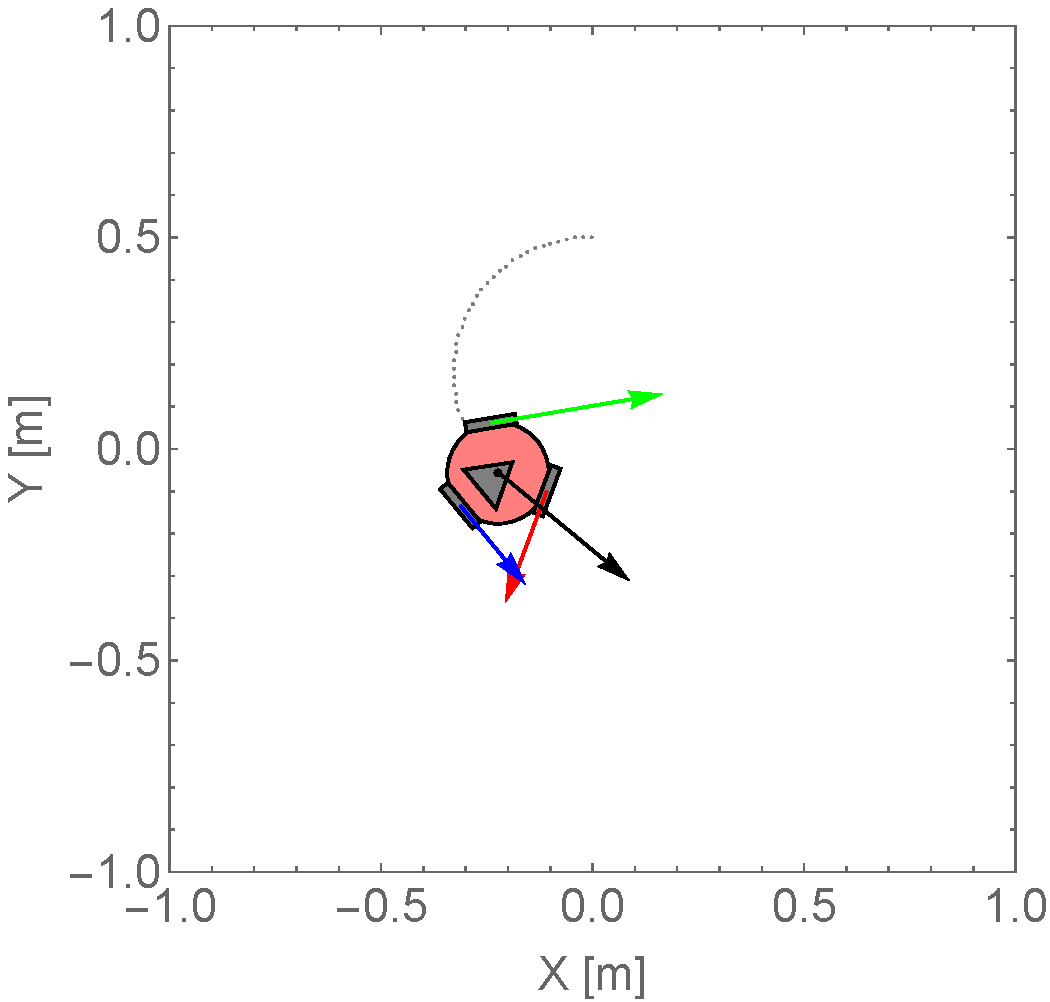
\includegraphics[height=5cm]{figures/2d_simulation/animations/2D_move_along_circle_rotating_reverse_direction/40}
	\caption{$0.40[s]$}
	\endminipage\hfill
	\minipage{0.33\textwidth}
	\centering
	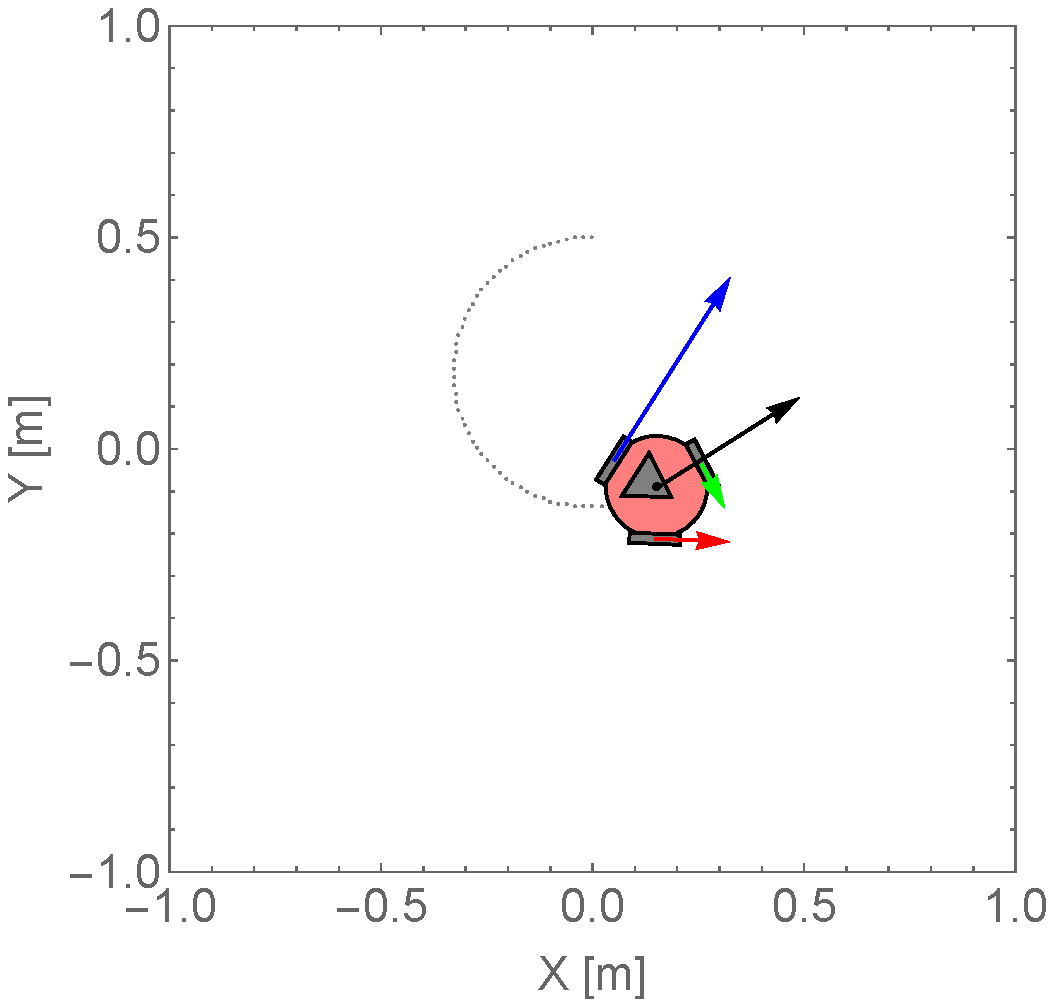
\includegraphics[height=5cm]{figures/2d_simulation/animations/2D_move_along_circle_rotating_reverse_direction/60}
	\caption{$0.60[s]$}
	\endminipage\hfill
\end{figure}
In this case also the robot orientation and also the speed direction is changing from step to step. The changed orientation ($\omega dt$) has to be considered in the equation of $\gamma$ as being defined in the local frame.\\[0.3cm] 
\noindent Moving along a line and changing the orientation:
\begin{itemize}
	\item $v^{i+1} = v^{i} = v^{0}$ (constant speed),
	\item $\omega^{i+1} = \omega^{i}<0$ (angular velocity),
	\item $\gamma^{i+1} = \gamma^i -\omega^i dt$ where $\dot \gamma$ is a constant.
\end{itemize}
\begin{figure}[htb!]
	\minipage{0.33\textwidth}
	\centering
	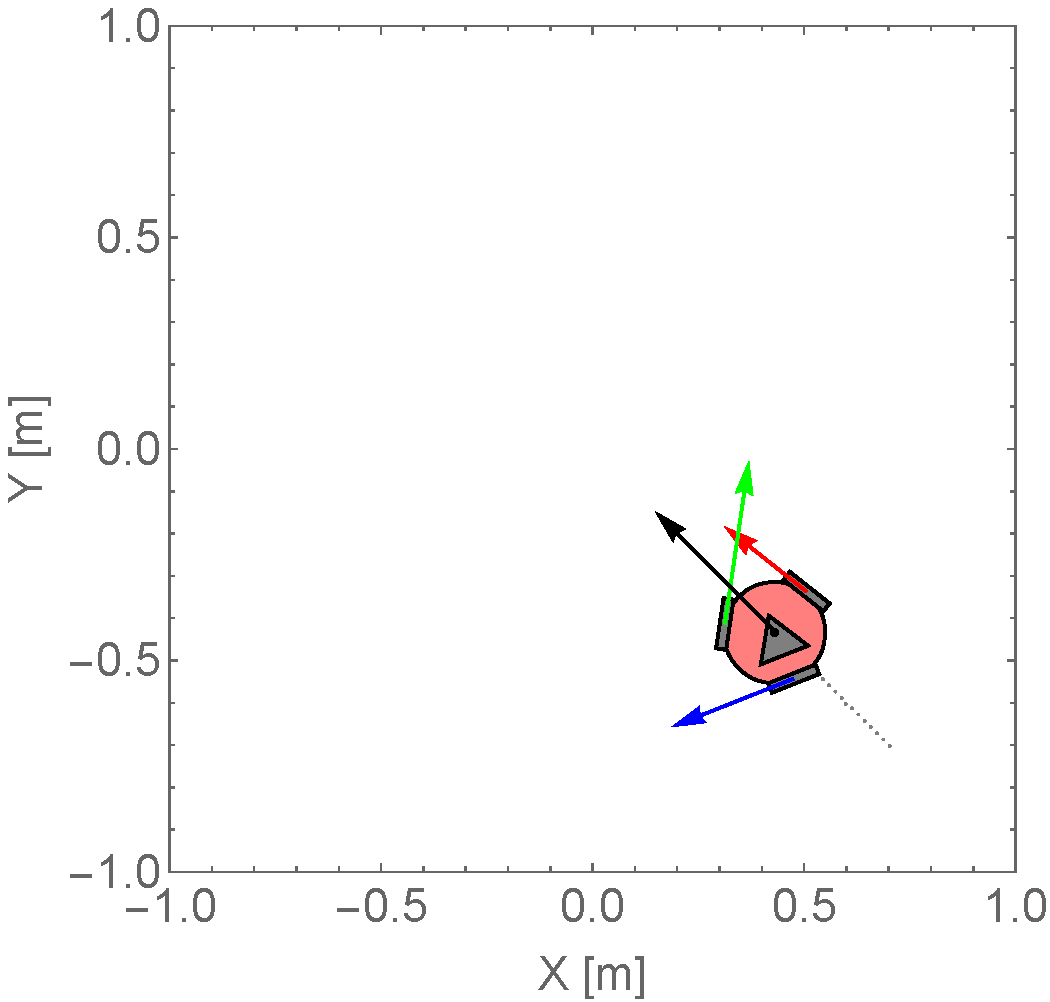
\includegraphics[height=5cm]{figures/2d_simulation/animations/2D_move_along_line_and_rotating/20}
	\caption{$0.20[s]$}
	\endminipage\hfill
	\minipage{0.33\textwidth}
	\centering
	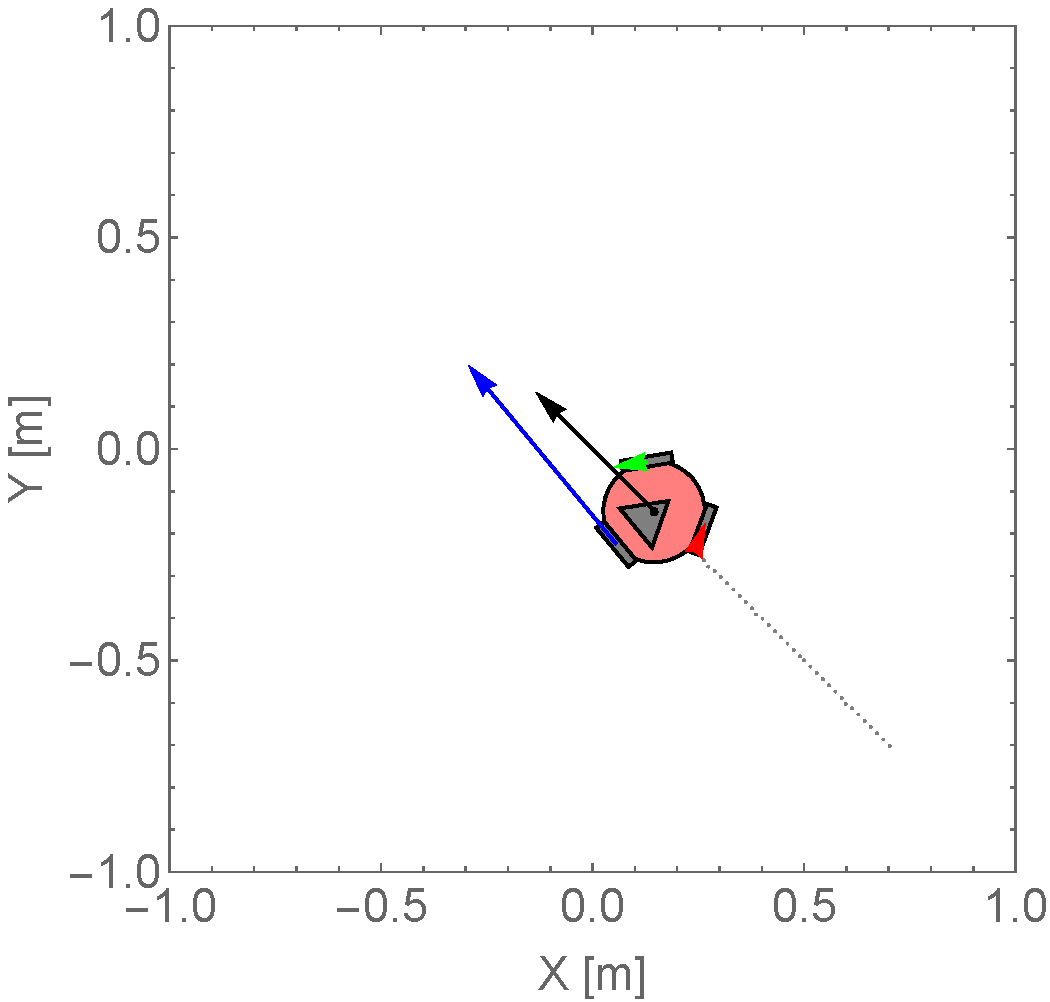
\includegraphics[height=5cm]{figures/2d_simulation/animations/2D_move_along_line_and_rotating/40}
	\caption{$0.40[s]$}
	\endminipage\hfill
	\minipage{0.33\textwidth}
	\centering
	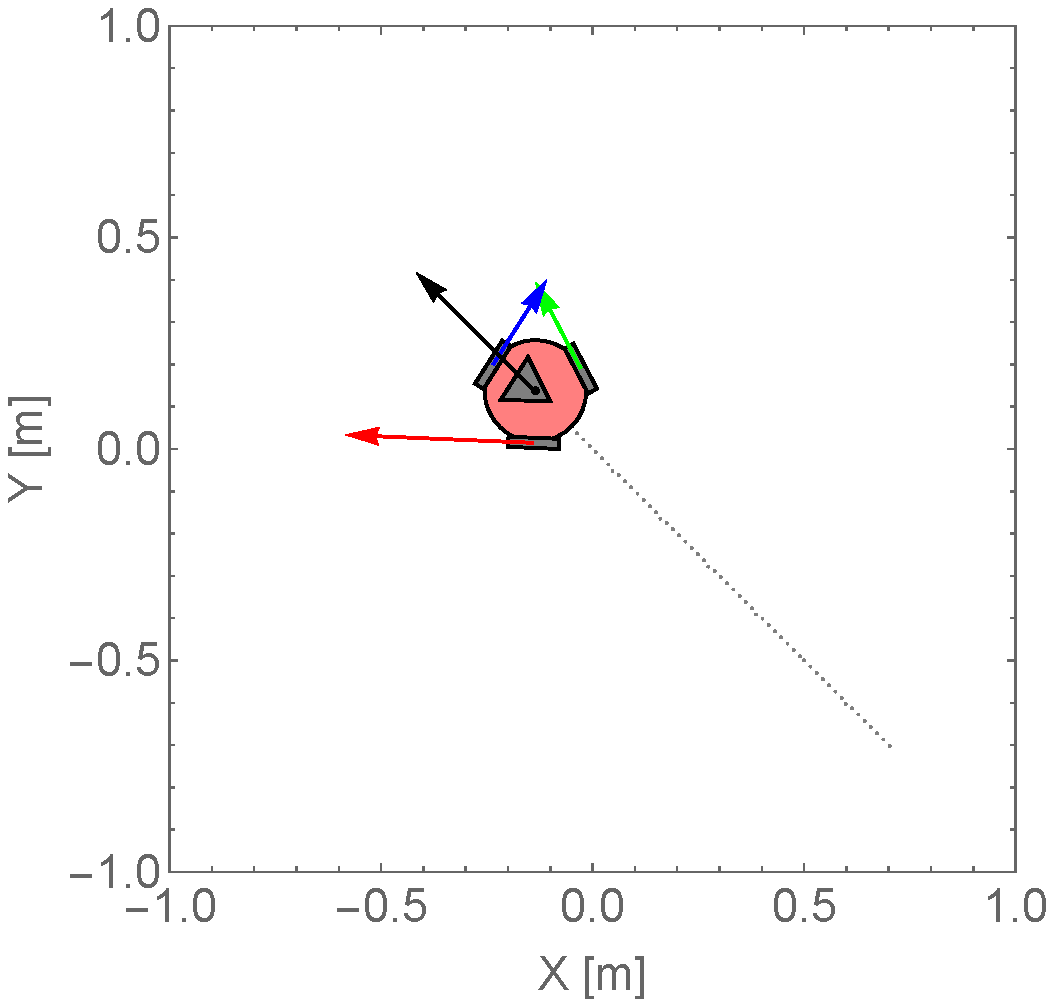
\includegraphics[height=5cm]{figures/2d_simulation/animations/2D_move_along_line_and_rotating/60}
	\caption{$0.60[s]$}
	\endminipage\hfill
\end{figure}
The kinematic simulation code is good tool to demonstrate the possibilites of such a robot configuration, but it does not give an analysis from dynamics point of view.
\newpage
\subsection{Dynamic analysis of DC motors}
\subsubsection{System modelling}
The robot configuration is equipped by three officially identical 12V DC motors with permanent magnets having the nominal rotational speed value of 107RPM at no load state. They have to be driven synchronously in order to obtain the desired movements. During operation the demand for having a variable motor speed is essential, thus control algorithm has to be developed. 
Briefly, the DC motor works on the principle (Lorentz Law) that when a current conductor wire (armature) is put in a magnetic field then it will be subjected to electromagnetic force in accordance with the direction and magnitude of current and magnetic field,i.e. $\mathbf{F} = I~\mathbf{l} \times \mathbf{B}$. The coil is connected to a DC power source, thus current will flow through the wire producing its own magnetic field. The mechanical force is produced as result of the magnetic field of the permanent magnets and the magnetic field of the coil. The magnetic field of the coil is attracted to the permanent magnetic field, therefore the armature starts rotating due to the induced electromagnetic force.
\begin{figure}[htb!]
	\centering
	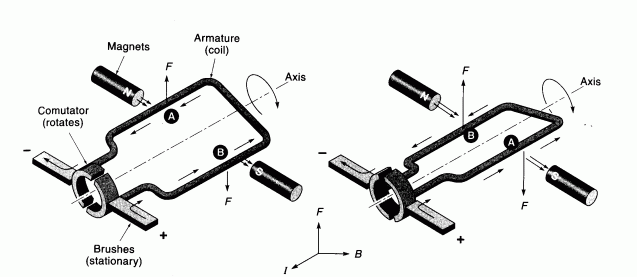
\includegraphics[height=4cm]{figures/dc_conducting_wire.png}
	\caption{A single current conductor in a static magnetic field \cite{dc_motor_2}}
	\label{dc_conducting_wire}
\end{figure}
At some point the magnetic fields would align resulting in a zero torque. In brushed DC motors this switching mechanism is done by the so called commutator part. The Figure \ref{dc_conducting_wire} represent a single wire with a commutator. The commutator is a simple mechanical switch that changes the polarity of the voltage put on the wire by touching the brushes in order to make the current flow in such a direction that maintains the direction of the generated torque, therefore the armature continue rotating. A single wire would provide a fluctuating torque during the operation since the angle between the coil and static magnetic flux is changing. For a more smooth operation of the rotor, several separate wire loops have to be used shifted from each other and switched one after the. This can be realised by applying more pairs of commutators which enables to connect always that coil loop with power source that does not align with the permanent magnetic field, thus can produce maximum torque. In practical motors the rotating part is called armature and standing part is called stator. The stator can be a permanent magnetic pole in case of small DC motors, while in larger motors an electromagnet is used which also powered by the same DC source in serial or parallel connection. In my case, the motor has a permanent magnetic stator.
According to Faraday's law of electromagnetic induction, a rotating loop of coil will produce an electromotive force called EMF. The case of the rotating armature loop is the same, thus in this case it produces an adverse electromotive force which is called back EMF that tends to decrease cause of the accelerating effect, i.e. the applied input voltage. As a result, the back EMF will decrease the armature current by a remarkable amount, thus the motor torque as well. \cite{dc_motor_1} \cite{dc_motor_2}

The electrical equivalent circuit of the armature and the free-body diagram of the rotor can be modeled as follows.
\begin{figure}[htb!]
	\centering
	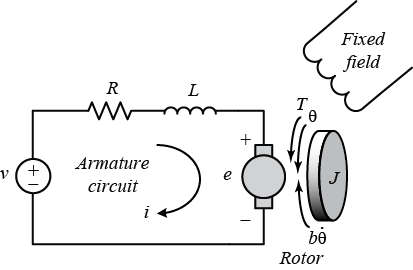
\includegraphics[height=5cm]{figures/dc_motor_model.png}
	\caption{DC motor electrical and mechanical model \cite{dc_motor_3}}
	\label{dc_motor_model}
\end{figure}

The motor is supplied with $V$ voltage as an input, while the output is the rotational speed of the rotor and shaft (rigid connection). In the mechanical model the load torque ($T_L$) and also dissipation energy is considered as being proportional with the angular speed. The motor torque is generally proportional to the armature current and the strength of the magnetic field, but in this model the magnetic field is assumed to be constant, thus the motor torque depends on the armature current ($i$) only. The back emf ($e$) is proportional to the angular velocity of the shaft. If SI units are used then the constants of the torque and the emf are equal, thus the same ($K$) constant can be used for the following equations:\cite{dc_motor_3}\cite{dc_motor_4}
\begin{equation}
T = K i
\end{equation}
\begin{equation}
e = K \dot \theta
\end{equation}		

Based on the model in Figure \label{dc_motor_model} the following equations can be derived by means of the Newtons's 2nd Law and Kirchoff's voltage law.
\begin{equation}
J \ddot \theta + b \dot \theta = K i - T_L
\end{equation}
\begin{equation}
L \frac{di}{dt} + R i = V - K \dot \theta
\end{equation}
The system can be described by a system of linear differential equations with respect to armature current and rotor angular velocity. A given system can be defined by 5 parameters, i.e. armature resitance (R), armature inductance (L), motor constant (K), damping constant (b) and motor inertia (J).
\subsubsection{DC motor parameter identification}
The motor parameters are essential to be known to develop a dynamic model. The L,J describes the dynamic behaviour of the motor, while the others characterize the system in a stationary aspect. Based on motor datasheet data (no load case, max efficiency case, max power case, stall torque case), only the stationary parameters can be estimated and you even cannot be sure about the values whether match the reality or not. Obviously, to get know about the dynamic parameters, measurements of dynamic operations of the motors are needed, e.g. measuring the step response to a given voltage. A robust technique for the parameter identification is to combine the measurement results with the capabilities of MATLAB Simulink and its Design Optimization tool. To carry out the following models and the parameter identificiation process the following references were considered: \cite{par_est_1}, \cite{par_est_2},\cite{par_est_3}. The Simscape library of the simulink makes it possible to make system models of coupled physical problems combining submodel elements, e.g. a DC motor which is an electromechanical system.
Firstly, in accordance with the equations above the following model was made.
\begin{figure}[htb!]
	\centering
	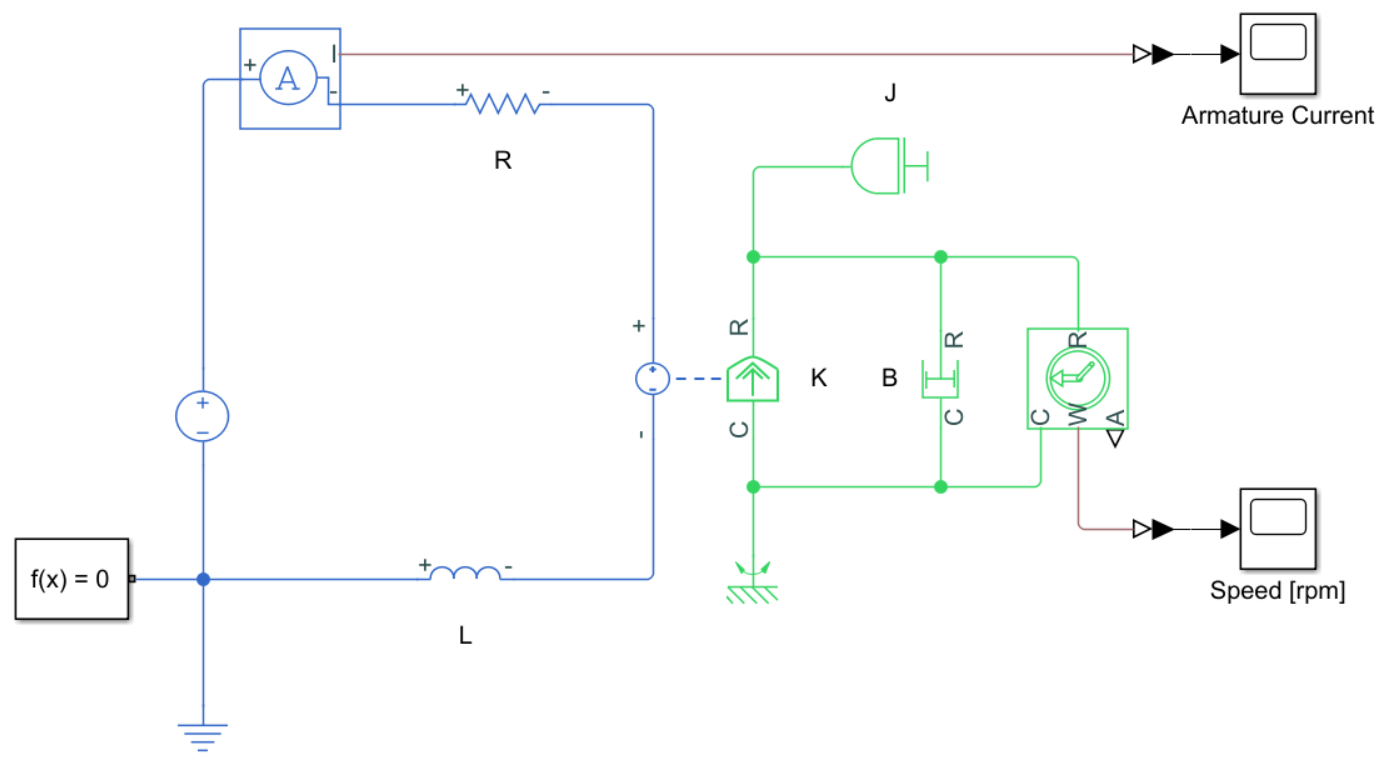
\includegraphics[height=5cm]{figures/simulink_dc_motor.png}
	\caption{Simple DC motor electromechanical model in Simulink}
	\label{simulink_dc_motor}
\end{figure}
The Figure \ref{simulink_dc_motor} represent the model in which the blue is the electrical circuit consisting a resistance $(R)$, inductance $(L)$, DC voltage source, electrical reference and current sensor, while the green elements are mechanical blocks, i.e. the inertia $(J)$, rotational damper $(B)$, rotational reference and a rotational speed sensor. The interface between the two domains is provided by the electromechanical converter which defines the $K$ constant. The $f(x)$ block defines solver settings for the numerical solution and the other two elements are blocks that monitors the current and shaft speed over time. This model has to match with equations above because actually those are solve numerically. The armature current has high peeks at the starting of DC motors due to the absence of the back emf which is proportional with rotational speed. The high gradients make the equation system to be stiff, thus ode15s solution method was chosen which a recommended one for such problems.

\begin{figure}[htb!]
	\centering
	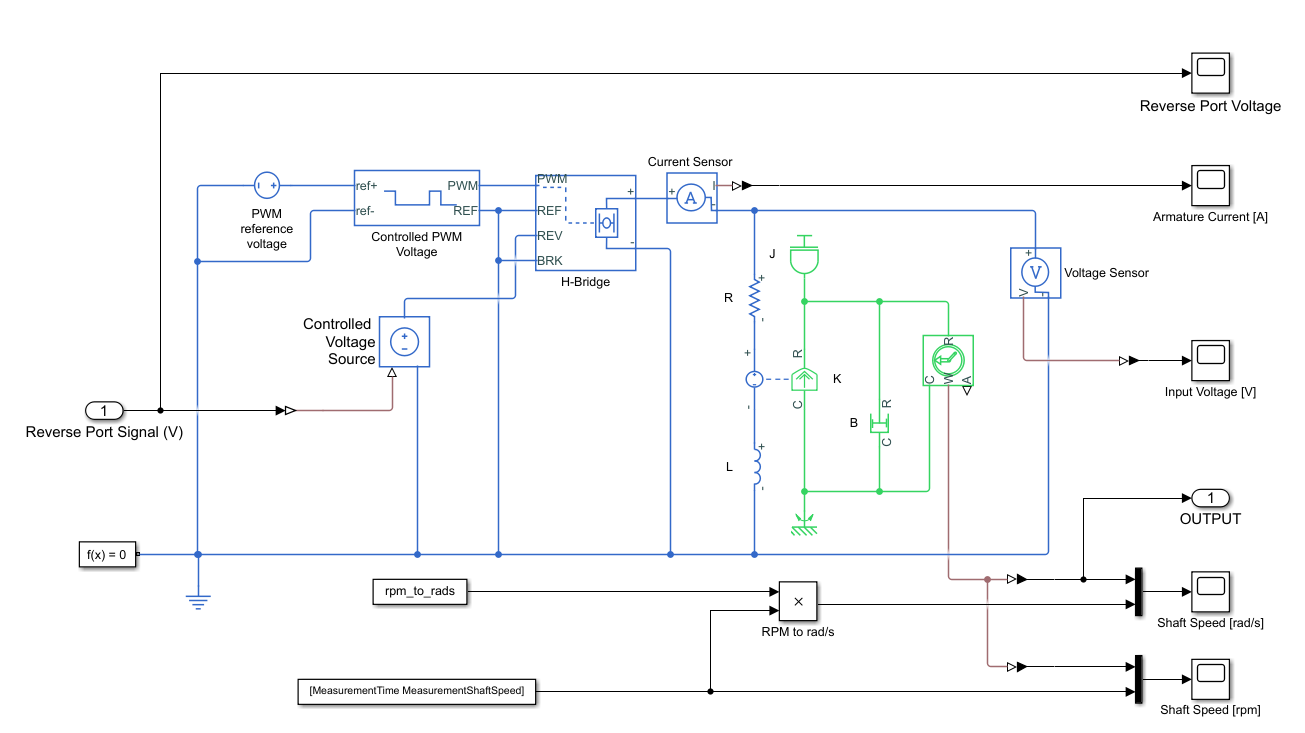
\includegraphics[height=8cm]{figures/simulink_dc_motor_complex.png}
	\caption{Complex DC motor electromechanical model in Simulink}
	\label{simulink_dc_motor_complex}
\end{figure}
In order to use the parameter estimation tool of the software, more complex voltage inputs have to defined. This model works with simple constant DC input voltage only. From the Simscape library, further electrical components can be added to the model such as the H-Bridge which can switch the rotational direction of the rotor or such as the PWM module which can produce a square wave with a given duty cycle to control the magnitude of the input voltage. The model shown in the Figure \ref{simulink_dc_motor_complex} has two inputs. One is the PWM reference signal which is a voltage value between 0 and 5V. The Controlled PWM unit generates from the reference signal a square wave which will be the input of the H-bridge motor drive component. This part can related to a voltage value of PWM type digital pin of the MCU. The following compoenent, the H-bridge motor drive, is actually the model of the L298N driver. Its magnitude of the output voltage is controlled by the PWM signal's duty cycle, while that of polarity is controlled by the digital signal at REV port. The second input of the model is Reverse Port Signal has to be a digital signal, thus 0V (LOW) correspond to no polarity change and 5V (HIGH) corresponds to switched polarity, thus reverse rotation of the rotor. The output of the model is shaft speed in rad/s. Transient operation of the system is provided by changing the reverse port digital signal. In order to make the parameter estimation, with the same inputs measurements for the output had to be taken before the simulation could be run. In addition, the parameters has to be initialized in the model as preliminary guess to have a combination of them to start the optimization from somewhere. Based the governing equations and motor data sheet values, a good initial guess could be given. In case of no load operation, $b=\frac{T}{\dot \theta}$ where $T=0.11$ [Nm] and $\dot \theta =11.21$ [rad/s] (107RPM), therefore $b=0.01[\frac{\text{Nms}}{rad}]$. Also other working points are known with respect to T-i values pairs, thus supposing linear relation the K can be estimated which was calculated to be 0.9338. Using these two values and supposing the steady state version of the Kirchoff law in case of no load, the resistance can be calculated as $R=\frac{V-K \dot \theta}{i} = 10.25$ [$\Omega$].
Considering all above, the initial guess of the seeked parameters is as follows:
$R=10[\Omega],~b=0.01[\frac{\text{Nms}}{rad}],~J=0.001[kgm^2],~L=0.01[H],~K=1$.
\begin{figure}[htb!]
	\centering
	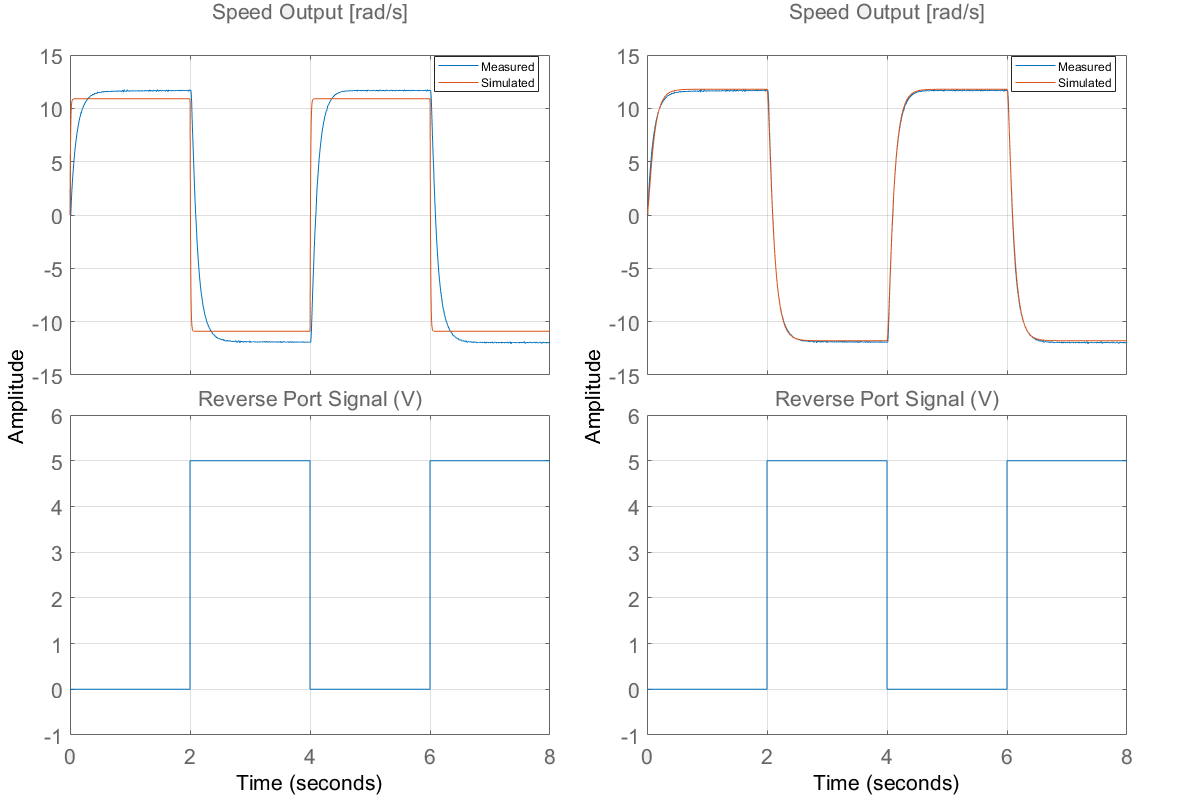
\includegraphics[height=10cm]{figures/simulink_par_est_1.png}
	\caption{Simulation results before and after the optimization}
	\label{simulink_par_est_1}
\end{figure}
 In the parameter estimation module both of the measurement and the simulation of the system can represented which is shown in the Figure \ref{simulink_par_est_1}. The plots on left side represent the simulation with the initial parameters. It can be seen that the steady-state value is close to the measured one, but the time-scales are quite different. The plot on the right side correspond to the optimized values which are the followings: $R=10[\Omega],~b=0.0197[\frac{\text{Nms}}{rad}],~J=0.0121[kgm^2],~L=0.166[H],~K=0.825[\frac{\text{Vs}}{rad}]$. The sum of squared errors were changed to be the cost function which converged from the initial value of 66.6 to 0.23 after 11 iterations. The obtained values are in a good relation with estimates, thus with the possible real values. The steady state current in the simulated free load case is 2 times higher, but the peak current is in a good order. Really high peaks can be extended when the polarity of the input voltage is switched, therefore higher torques that can be expected during such operations which means more risk for fall-over. The initial peak current can be estimated as $U/R = 12[V]/10.25[\Omega] = 1.17 [A]$ assuming zero initial shaft speed. Figure \ref{simulink_armature_current} shows similiar current peaks in the simulation.
 \begin{figure}[htb!]
 	\minipage{0.45\textwidth}
 	\centering
 	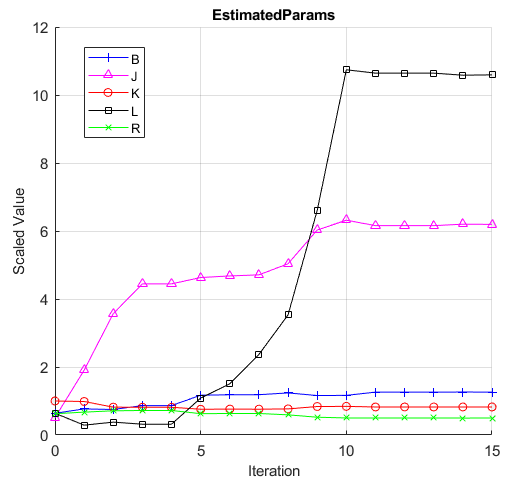
\includegraphics[height=7cm]{figures/simulink_par_est_2.png}
 	\caption{Iterations of estimated parameters}
 	\endminipage\hfill
 	\minipage{0.45\textwidth}
 	\centering
 	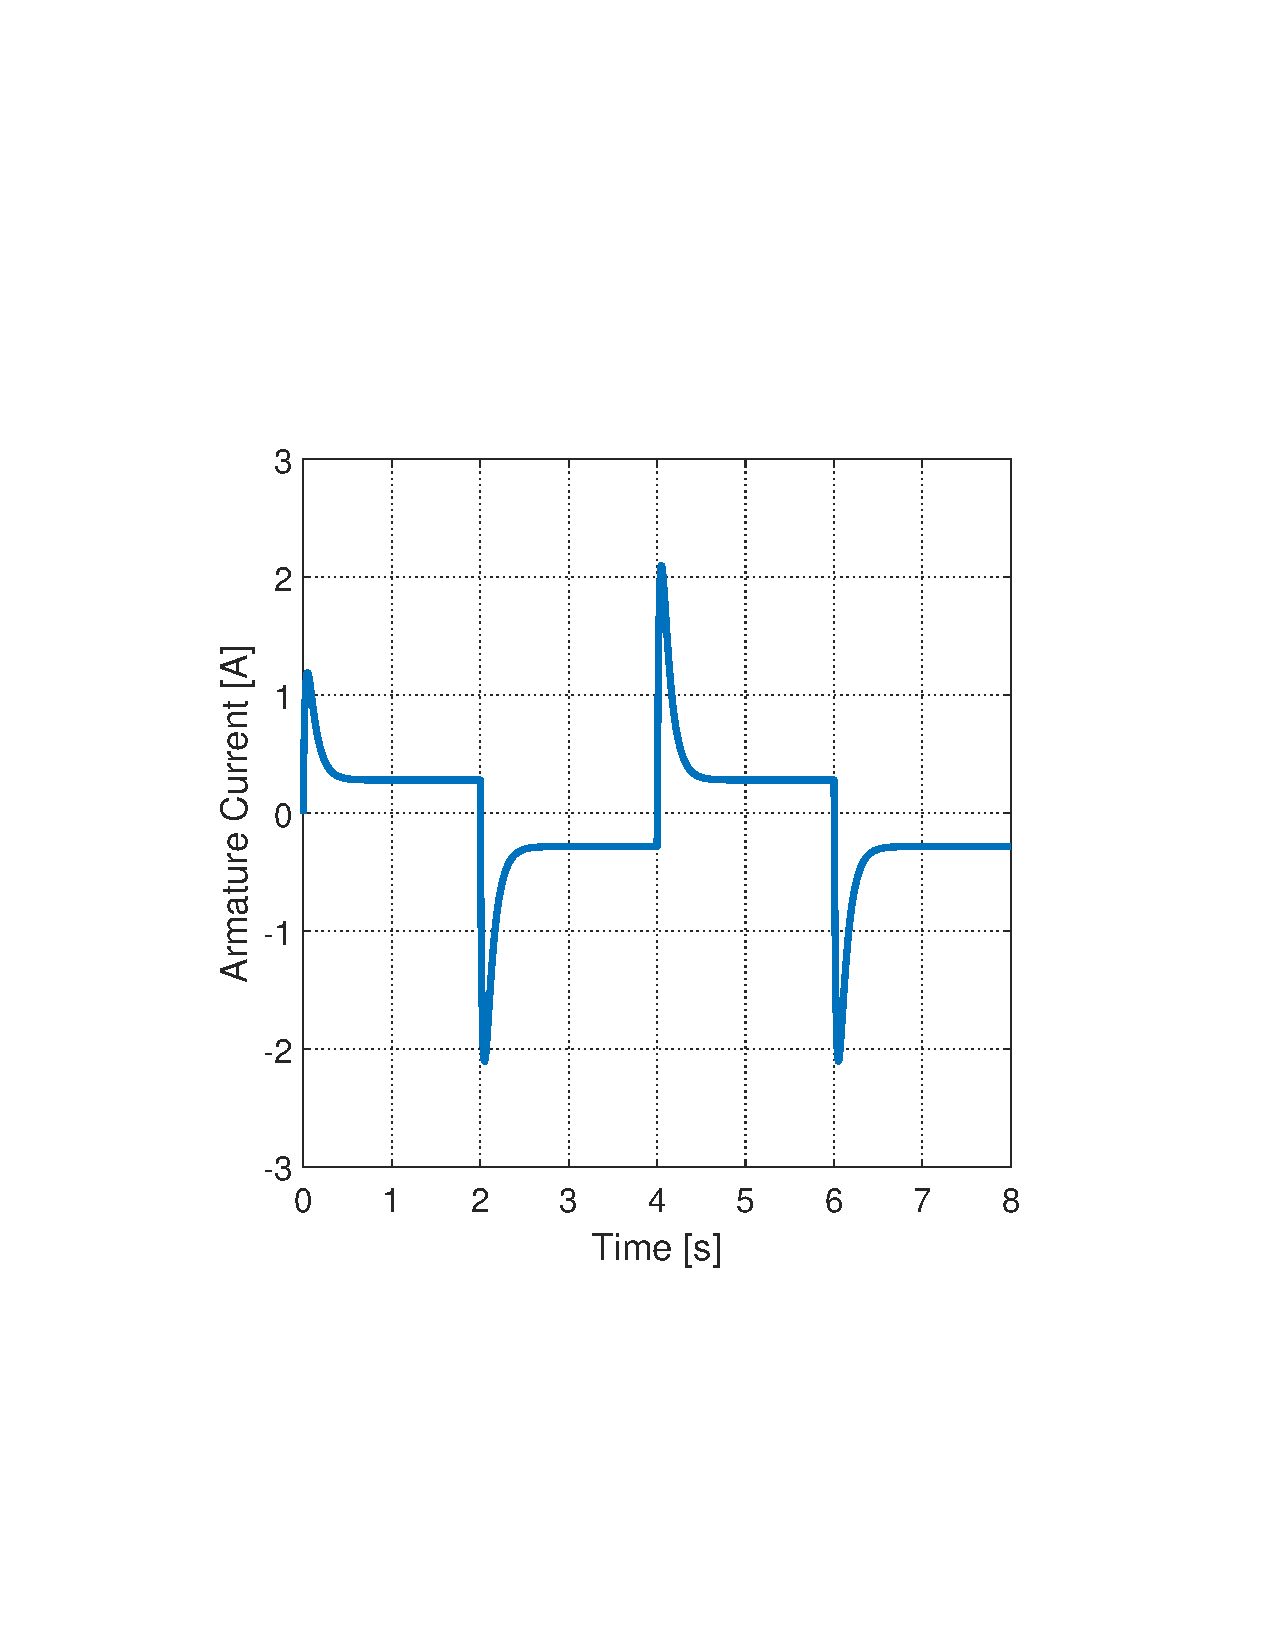
\includegraphics[height=7cm]{figures/simulink_armature_current}
 	\caption{Aramature current of the optimzed model}
 	\label{simulink_armature_current}
 	\endminipage\hfill
 \end{figure}
The solution method was got numerically while the dynamic model of the robot is fully analytic and generally a more simple method is seeked that might be implemented also in the hardware code, thus it would be more convenient to find a good analytical formula too calculate the current, thus the motor torques exerted on the wheels. Firstly, in a similar way the numerical solution of the governing equations were implemented. Because of the high current peaks, implicit Euler-method was chosen combined with Newton-Raphson iterations because the built-in solver could not handle stiffness of the equation properly. The chosen method calculated the same dynamics for the system as the numerical solution in Simulink. Considering the governing equations, it can be said that let us omit the inductance of the armature, thus the "inertia" of the electric circuit. With this assumption combining the two constitutive equations, the following first-order linear differential equation can be derived:
\begin{equation}
	b \omega(t)+\theta \dot \omega(t)=\frac{K (V-K \omega(t))}{R},
\end{equation} 
which solution is:
\begin{equation}
	\omega(t) = \frac{e^{-\frac{b t}{\theta }-\frac{K^2 t}{\theta  R}} \left(K V e^{\frac{t \left(b R+K^2\right)}{\theta  R}}+b R \text{$\omega_0 $}+K^2 \text{$\omega_0 $}-K V\right)}{b R+K^2}
\end{equation}
where $\omega_0$ is the initial angular speed.
The armature current can be extracted as
\begin{equation}
	i_a(t) =\frac{V-K\dot \theta}{R}.
\end{equation}
The Figure \ref{mahemetica_comparision_1} and \ref{mahemetica_comparision_2} depict the numerical and analytical solution for the shaft speed [rad/s] and armature current [A] where the oranges solid line is the analytical and dashed black is the numerical solution.
 \begin{figure}[htb!]
	\minipage{0.45\textwidth}
	\centering
	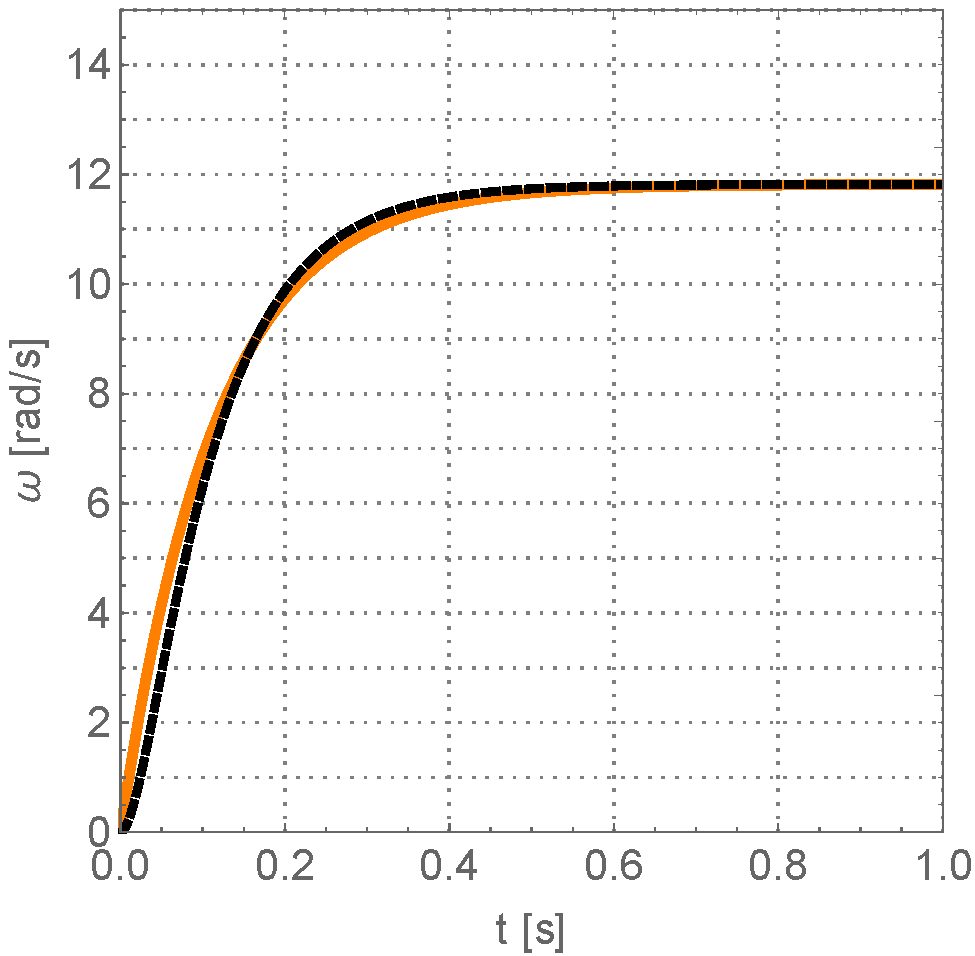
\includegraphics[height=7cm]{figures/mahemetica_comparision_1}
	\caption{Angular velocity}
	\label{mahemetica_comparision_1}
	\endminipage\hfill
	\minipage{0.45\textwidth}
	\centering
	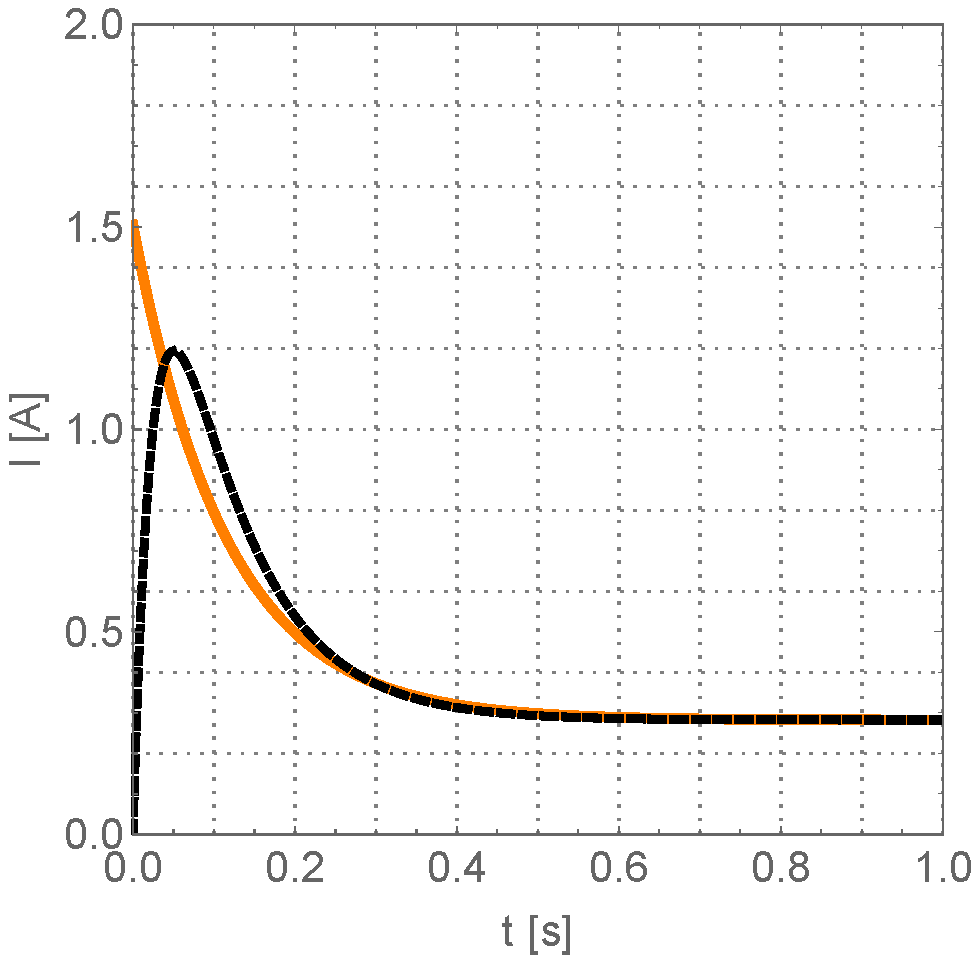
\includegraphics[height=7cm]{figures/mahemetica_comparision_2}
	\caption{Armature current}
	\label{mahemetica_comparision_2}
	\endminipage\hfill
\end{figure}
The analytical solution is in a good match with the more accurate numerical one (L is not assumed to be zero) and also higher current is estimated at start which is an conservative engineering approach. In this way, it is a good estimation to work with the analytical formula in the dynamic model of the robot.

\newpage
\subsection{Coupled dynamic model of the robot}
 \begin{figure}[htb!]
	\minipage{0.45\textwidth}
	\centering
	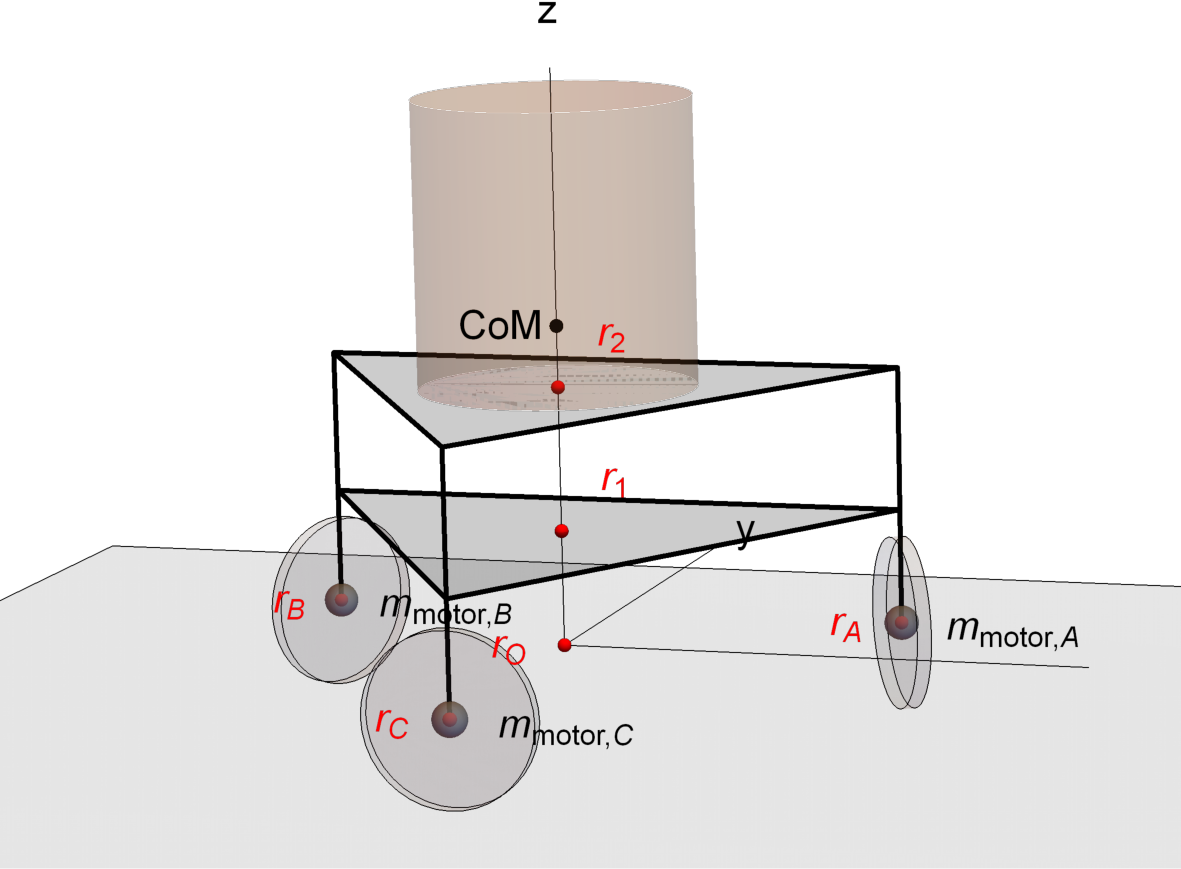
\includegraphics[height=7cm]{figures/robotModel}
	\caption{Angular velocity}
	\label{robotModel}
	\endminipage\hfill
	\minipage{0.45\textwidth}
	\centering
	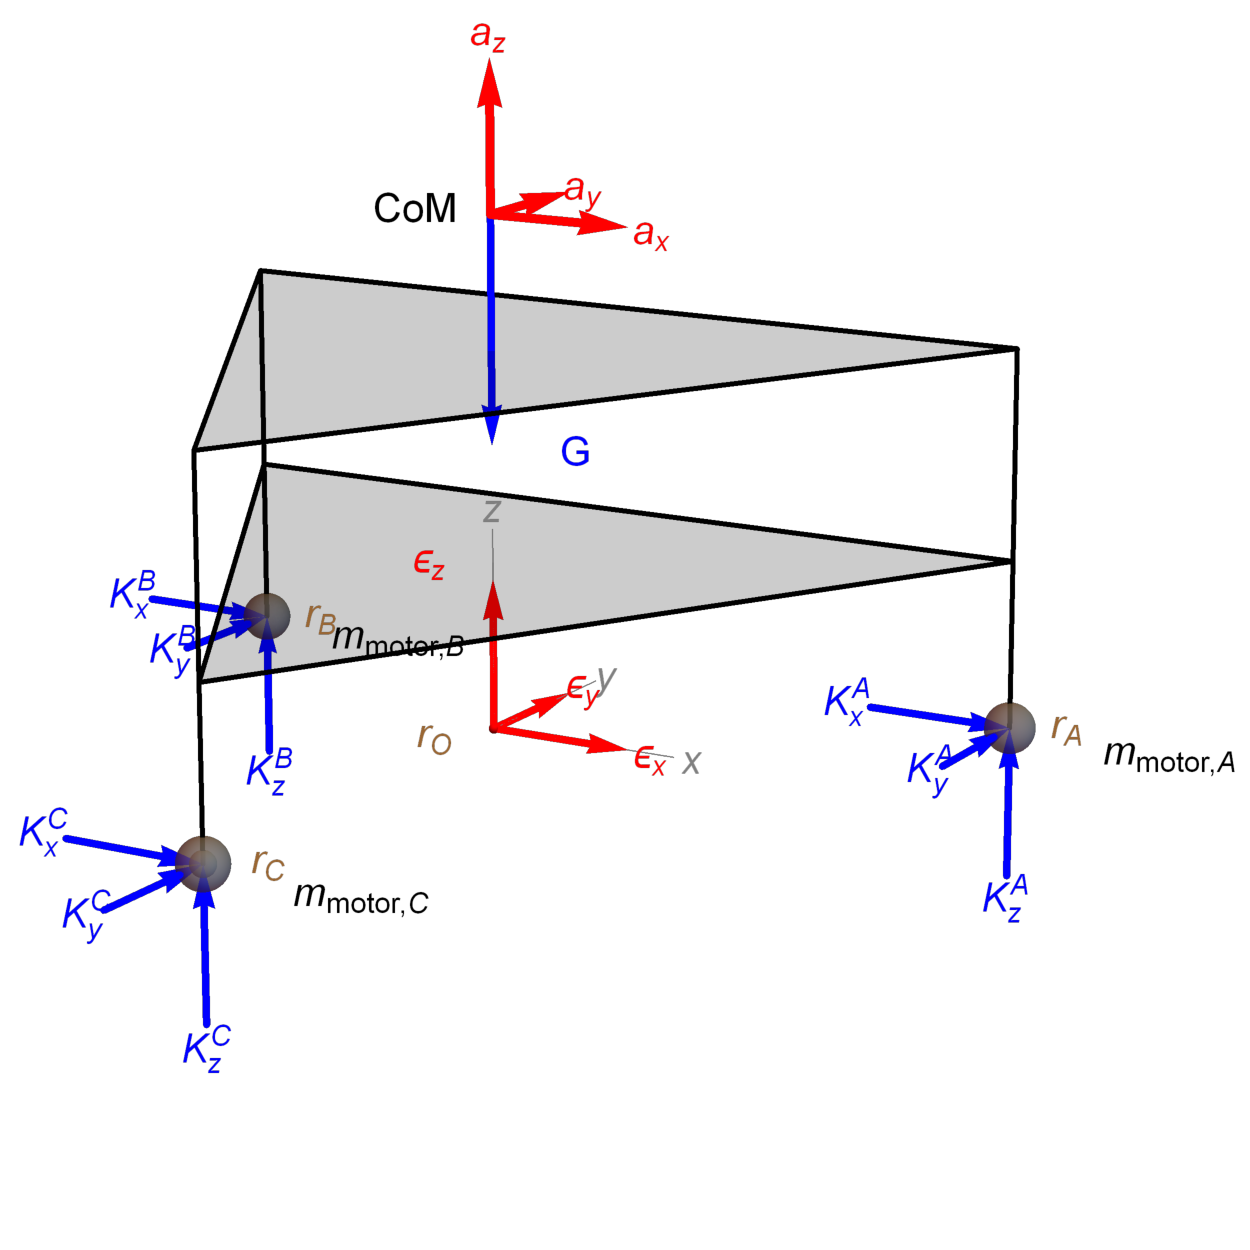
\includegraphics[height=8cm]{figures/caseFBD}
	\caption{Armature current}
	\label{caseFBD}
	\endminipage\hfill
\end{figure}
\begin{figure}[htb!]
	\minipage{0.45\textwidth}
	\centering
	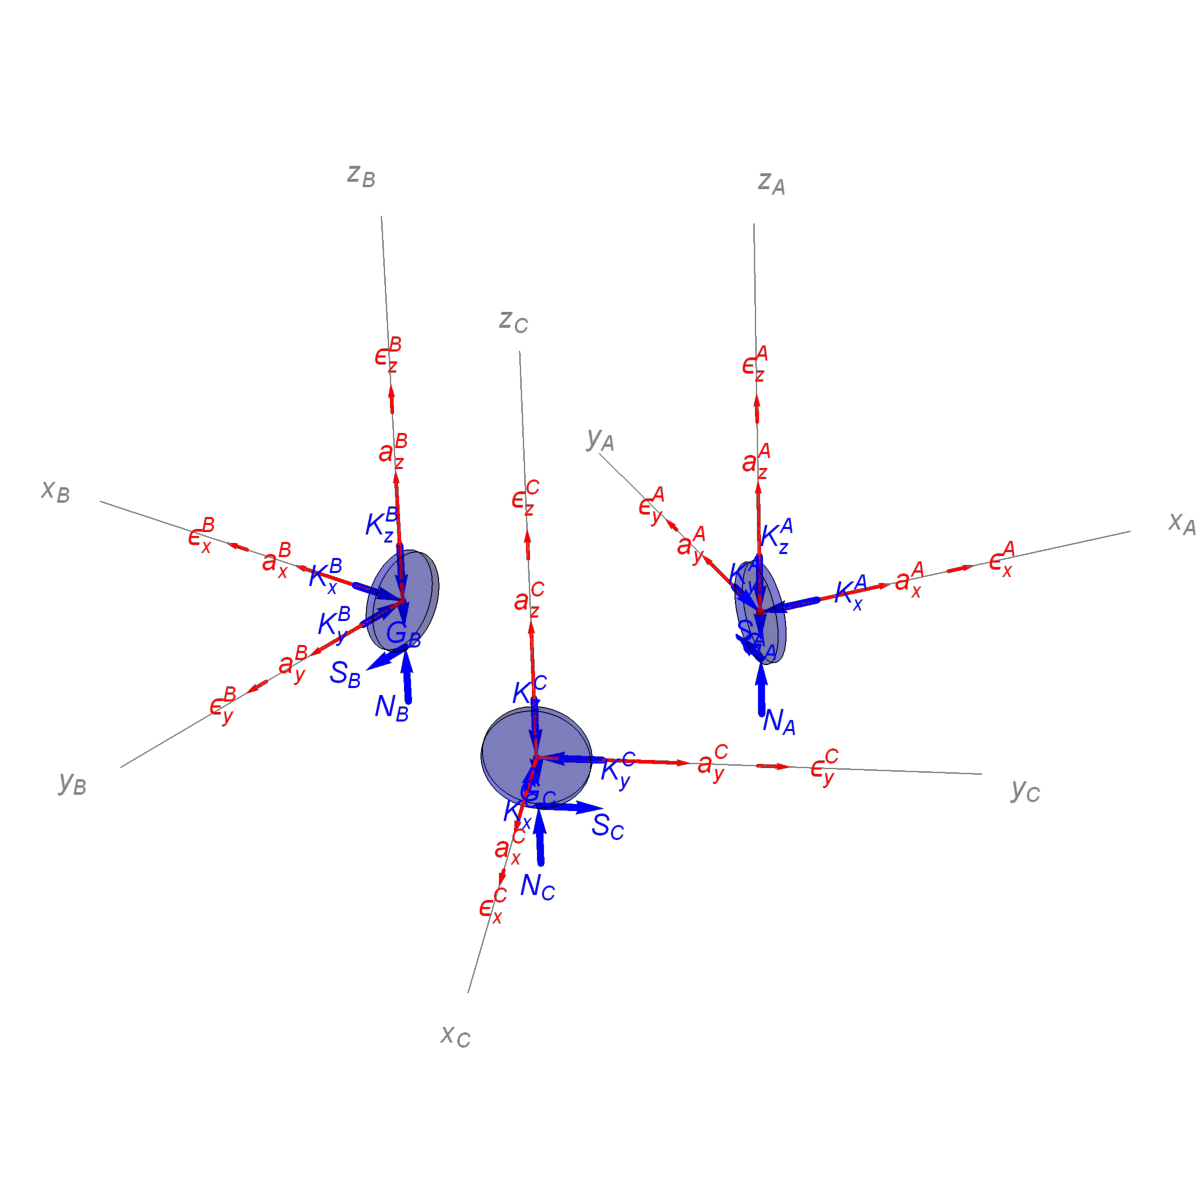
\includegraphics[height=8cm]{figures/wheelsFBD}
	\caption{Angular velocity}
	\label{wheelsFBD}
	\endminipage\hfill
	\minipage{0.45\textwidth}
	\centering
	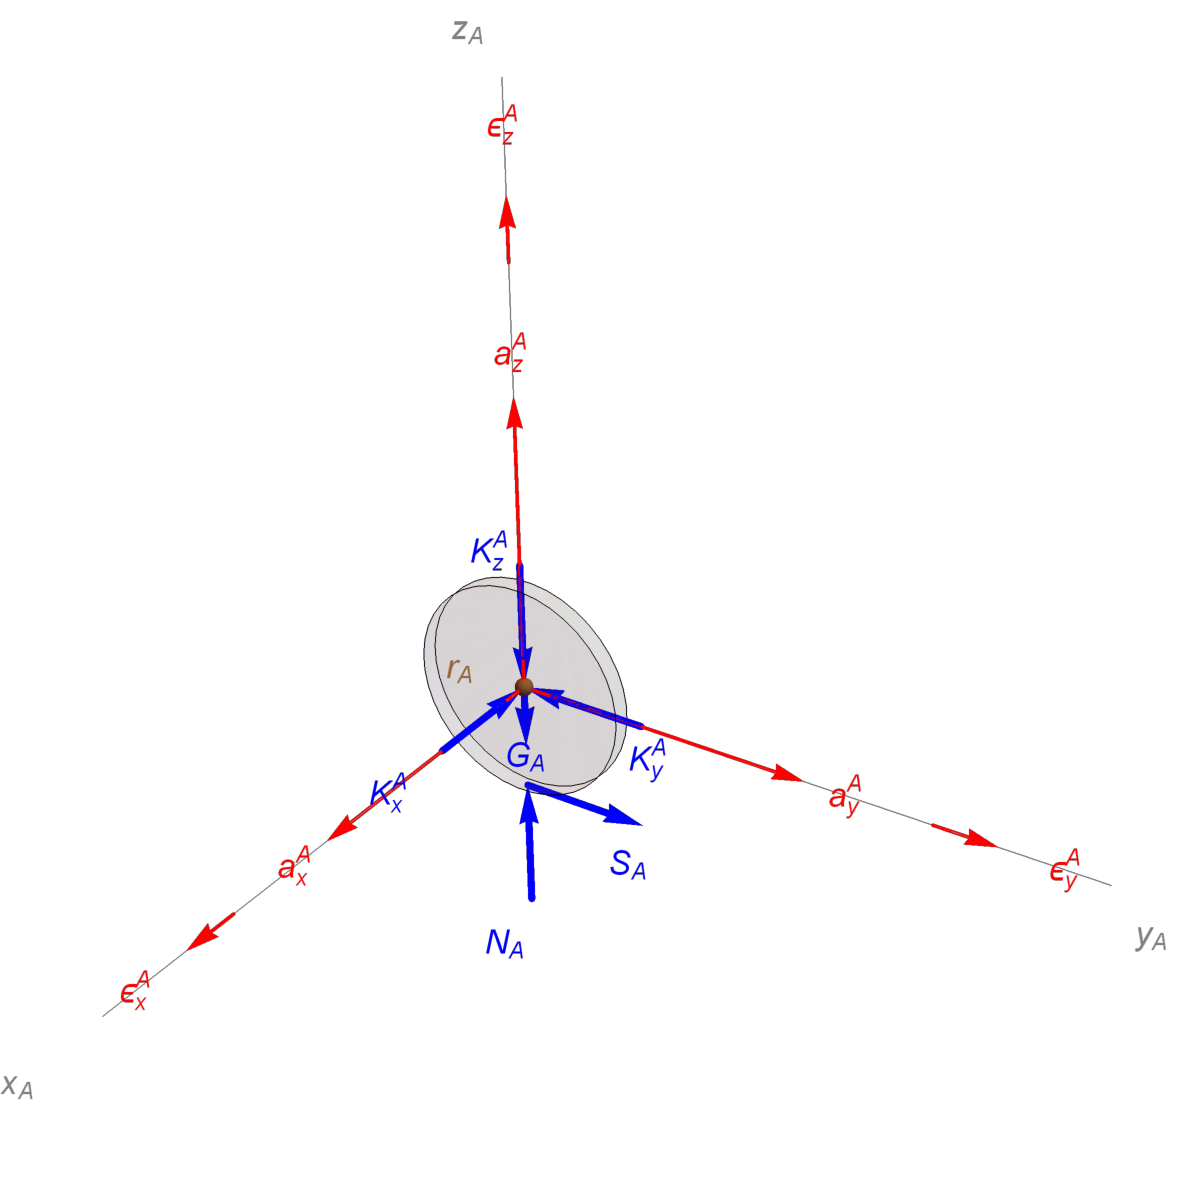
\includegraphics[height=8cm]{figures/wheelFBD}
	\caption{Armature current}
	\label{wheelFBD}
	\endminipage\hfill
\end{figure}
\newpage

\subsection{DC motor speed analysis}

\subsubsection{Step response analysis of the motors}
The motors are to be controlled via PWM and with the help of the rotary encoders the response function to any voltage value could be measured. It is more convenient to treat the PWM signal's duty cycle as the control input athough voltage level is applied to the armature of the motor. Firstly, let the pwm value be regarded as an input and the wheel speed as an output assuming that the transfer function of the gearbox and power electronic module are proportional type, thus it can be handled together with the motor as a plant element.
\begin{figure}[htb!]
	\centering
	\includegraphics[height=7cm]{figures/directed_speed_pwm_100}
	\caption{PWM=100\% step response of the motors}
	\label{directed_speed_pwm_100}
\end{figure}
The motors gave quite similar responses with respect to time constant and amplitude and also the nominal value (107RPM at 12V no load case) was also obtained with small deviations.

\begin{figure}[htb!]
	\centering
	\minipage{0.32\textwidth}
	\centering
	\includegraphics[height=5cm]{figures/directed_speed_pwm_60}
	\caption{PWM=60\% step response of the motors}
	\endminipage\hfill
	\minipage{0.32\textwidth}
	\centering
	\includegraphics[height=5cm]{figures/directed_speed_pwm_40}
	\caption{PWM=40\% step response of the motors}
	\label{mecanum}
	\endminipage\hfill
	\minipage{0.32\textwidth}
	\centering
	\includegraphics[height=5cm]{figures/pwm_u}
	\caption{PWM=40\% step response of the motors}
	\label{mecanum}
	\endminipage\hfill
\end{figure}
Unfortunately, the problems were captured when the duty cycle of the pwm signal was decreased. Firstly, the prior guess that the pwm value provided in the MCU code will be proportional to the motor speeds was proven to be wrong. Furthermore one of the L298N module was functioning really poorly as it provided different voltage values for the same pwm signal which resulted that the Motor C was spinning remarkably slower. It is also clearly visible that the system is nonlinear as neither for the Motor A and B are the same dynamics with respect to rise time are obtained, thus even the shape is not similar.
It is very straight forward that without proper control of the wheels it is impossible to achieve smooth and accurate movements. As a first approximation, it is worth neglecting the mentioned issues and handle the system as it would be completely linear. Problems could occur at low voltages where the system probably become extremely nonlinear as the motor will not move at small voltages due to the sticking friction. In the model only the linearly modeled viscous friction is included. A possible solution is to have the motor banned to work in this region. 
\subsubsection{Controller design using blackbox model \cite{dc_motor_3}}
Considering above all, based on the response function of the maximum pwm signal a controller can be designed for the whole range for each wheel separately. In order to do this, a black box model has to constructed. In case of DC motor it is a typical procedure to handle the system as a first order one. \cite{dc_motor_3} 
The governing equations for the DC motor are the followings:
\begin{equation}
J \ddot \theta + b \dot \theta = K i
\end{equation}
\begin{equation}
L \frac{di}{dt} + R i = V - K \dot \theta
\end{equation}
Applying the Laplace transform and rearranging the transformed equations the transfer function of the system is as follows:
\begin{equation}
T(s) = \frac{\dot \theta (s)}{V(s)} = \frac{K}{(Js+b)(Ls+R)+K^2}.
\end{equation} 
Beside the fact that a second-order model can be derived, the step response of the motor looks like that of a first-order system. After inspecting the actual step response of these motors, this looks as a good approximation. The reason for that the motor is an overdamped second-order system, thus it has two negative poles (roots of the denominator of the transfer function). The system is stable and has two time constants. In case of DC motors, the time constant of the mechanical dynamics is much higher compared to the time constant of the electrodynamics, thus the slower mechanical dynamics dominates the time response. 
A first order system can be expressed as it follows:
\begin{equation}
	P(s) = \frac{\dot{\theta(s)}}{DC(s)}= \frac{k_{dc}}{1+\tau s},
\end{equation}
where
\begin{itemize}
	\item $\tau$ - time constant which equals the time it takes the system to reach the 63.2\% of steady-state step response of a unit step, more generally it represents the time scale of the system dynamics
	\item $k_{dc}$ - DC gain, the ratio of the magnitude of the steady-state step response to the magnitude of the step input
\end{itemize}
Based on the measurments shown in Figure \ref{directed_speed_pwm_100} the following values were calculated providing a really good agreement.
\begin{table}[h]
	\centering
	\label{first_order_model_table}
	\begin{tabular}{|c|c|c|c|}
		\hline
							& A  		& B  		& C   		\\ \hline
		$\tau$ {[}s{]} 		& 111.05 	& 113.39 	& 109.07 	\\ \hline
		$k_{dc}$ {[}rpm{]}       & 100.70 	& 99.88 	& 107.03   	\\ \hline
	\end{tabular}
	\caption{First-order model parameter estimations}
\end{table}
A common choice for such a system is a PI controller.\cite{dc_motor_3} The plant block is overall model of the power electronic module, the motor armature, rotary encoders and the signal processing on the MCU. 
\begin{figure}[htb!]
	\centering
	\includegraphics[height=4cm]{figures/dc_motor_closed_system}
	\caption{Model of the closed (feedback controlled) system}
	\label{dc_motor_closed_system}
\end{figure}
The transfer function of the controller is as follows:
\begin{equation}
C(s) = K_p + \frac{K_i}{s}.
\end{equation}
The transfer function of the (positive feedback) closed-loop:
\begin{equation}
T(s) = \frac{C(s)P(s)}{1+C(s)P(s)}=\frac{A (K_i+K_p s)}{A K_i+A K_p s+s^2 \tau +s}
\label{eq_transfer_function}
\end{equation}
The closed-loop system is almost a second-order one except for the presence of the zero (possible root in the denominator), thus it does not match with the canonical exactly:
\begin{equation}
G(s) = \frac{{k_{dc}\omega_n}^2}{s^2 + 2 \zeta \omega_n s +{\omega_n}^2}
\label{eq_transfer_function_canonical}
\end{equation}
where
\begin{itemize}
	\item $k_{dc}$ - DC gain is the ratio of the magnitude of the steady-state step response to the magnitude of the step input,
	\item $\zeta$ - The damping ratio is a dimensionless quantity characterizing the rate at which an oscillation in the system's response 		decays due to effects such as viscous friction or electrical resistance,
	\item $\omega_n$ - The natural frequency is the angular frequency that the system will oscillate at when there is no damping. \cite{dc_motor_3}
\end{itemize}

The original system is overdamped but the addition of a proportional controller can make it underdamped as it has similar behaviour like "virtual spring". For such special case several design equations are available if the parameters in the canonical form are known. The presence of the zero in closed-loop transfer function can be a cause of errors. However, as a first guess it can provide a good approximation for starting value for the controller if the presence of zero is not considered and the system is treated as if it was an underdamped second-order system.
It is important to mention, that the closed-loop system would have a canonical form if only proportional type controller was used.


The canonical second-order transfer function has two poles at:
\begin{equation}
s_p = -\zeta \omega_n \pm j \omega_n \sqrt{1-{\zeta}^2} = -\sigma \pm j\omega_d.
\label{eq_poles}
\end{equation}
If $\zeta<1$, then the system is underdamped, the two poles are both complex-valued with negative real parts. The system is asymptotically stable and oscillating with the damped natural frequency $\omega_d = \omega_n \sqrt{1-{\zeta}^2}$. Based on the value of damping the system can marginally stable and unstable, but those are not the cases which are have to be examined now.

Combining the denumerators of equation (\ref{eq_transfer_function}) and (\ref{eq_transfer_function_canonical}) the following expressions can be obtained:
\begin{equation}
	{\omega_n}^2 = \frac{A K_i}{\tau},
\end{equation}
\begin{equation}
	2\omega_n\zeta  = \frac{1+A K_p}{\tau}.
\end{equation}
Additionally using the equation \ref{eq_poles}, the relation between the poles of the closed loop and the controller parameters can be derived:
\begin{equation}
	%{\omega_d}^2 = \frac{A K_i (1-\zeta^2)}{\tau},
	\sigma^2 + {\omega_d}^2 = \frac{A K_i}{\tau},
	\label{eq_pi_from_poles_1}
\end{equation}
\begin{equation}
	\sigma = \frac{1+A K_p}{2\tau}.
	\label{eq_pi_from_poles_2}
\end{equation}

The figure \ref{second_order_underdamped_response} represents the step response of a canonical second order system and several properties are denoted to characterize itself.
\begin{figure}[htb!]
	\centering
	\includegraphics[height=7cm]{figures/step_response_of_2nd_order_system_1}
	\caption{Step response characteristics}
	\label{second_order_underdamped_response}
\end{figure}

\begin{itemize}
	\item Settling Time is time that the system needs to have an output with a smaller deviation from the steady-state in terms of a given percentage. In case of second-order canonical system the following formula provides a good approximation:
	\begin{equation}
	T_s = -\frac{ln(tolerance)}{\zeta \omega_n} = -\frac{ln(tolerance)}{\sigma}
	\label{eq_settling_time}
	\end{equation}
	\item Percent Overshoot characterize the output in terms of the ratio of maximum peak and the steady-state value expressed as a percentage.
	\begin{equation}
	Mp = e^{\frac{-\zeta \pi}{\sqrt{1-\zeta^2}}}
	\label{eq_overshoot}
	\end{equation}
	The corresponding peak time is as follows:
	\begin{equation}
	T_p = \frac{\pi}{\omega_d}
	\label{eq_overshoot_time}
	\end{equation}
\end{itemize}
Ideally closed-loop respond with low settling time and overshoot is wanted. Limits can be defined in arbitrary way that suits are demands with respect to the former properties. Based on equations \ref{eq_settling_time}, \ref{eq_overshoot} and \ref{eq_overshoot_time} further limits can be derived for $\zeta$ and $\omega_d$.
\begin{itemize}
	\item 1 \% settling time:
	\begin{equation}
	T_s = -\frac{ln(0.01)}{\sigma} = \frac{4.605}{\sigma} < l_{T_s},
	\end{equation}
	\begin{equation}
	\sigma > \frac{4.605}{l_{T_s}}.
	\end{equation}
	
	\item peak time:
	\begin{equation}
	T_p = \frac{\pi}{\omega_d} < l_{T_s},
	\end{equation}
	\begin{equation}
	\omega_d > \frac{\pi}{l_{T_p}}.
	\end{equation}
	
	\item maximum percent overshoot:
	\begin{equation}
	Mp = e^{\frac{-\zeta \pi}{\sqrt{1-\zeta^2}}}  < l_{M_p},
	\end{equation}
	\begin{equation}
	\zeta > \sqrt{\frac{ln^2(l_{M_p})}{\pi^2+ln^2(l_{M_p})}}.
	\end{equation}
\end{itemize}
where $l_{T_s}$, $l_{T_p}$ and $l_{M_p}$ are the limits respectively.
Considering the provided limits, some guidelines for seeking suitable poles can be obtained which probably result desired system dynamics. Rearranging the equations \ref{eq_pi_from_poles_1} and \ref{eq_pi_from_poles_2}, the controller gain estimations can be calculated:
\begin{equation}
	K_p = \frac{2 \sigma \tau - 1}{A},
\end{equation}
\begin{equation}
	K_i = \frac{\tau(\sigma^2 + {\omega_d}^2)}{A}.
\end{equation}
As it was mentioned before, choosing the poles based on the above limits can not guarantee acceptable system behaviour as our system is not a canonical second-order, on the top of that the plan model is also simplified to a first order.
\begin{figure}[htb!]
	\centering
	\includegraphics[height=7cm]{figures/possible_poles}
	\caption{Pole parameter field considering the limits}
	\label{possible_poles}
\end{figure}
The figure above shows the possible real and imaginary value pairs which satisfies the requirements. The real part of pole is $\sigma$, the imaginary part is $\omega_d$ and the angle $beta$ can calculated by means of $\zeta = cos(\beta)$.
Let us have the following requirements:
\begin{itemize}
	\item Settling time for 1$\%$: 2[s]
	\item Peak time: 1[s]
	\item Max peak amplutude: 10\%
\end{itemize}
and let us use measurments corresponding to pwm value of 0.5. After fitting the first order balck box model the following values were obtained.
\begin{table}[h]
	\centering
	\label{first_order_model_table_50}
	\begin{tabular}{|c|c|c|c|}
		\hline
		& A  		& B  		& C   		\\ \hline
		$\tau$ {[}s{]} 		& 0.2949 	& 0.2880 	& 0.3767 	\\ \hline
		$k_{dc}$ {[}rpm{]}       & 93.8978 	& 94.9998 	& 80.5325   	\\ \hline
	\end{tabular}
	\caption{First-order model parameter estimations}
\end{table}
\begin{figure}[htb!]
	\centering
	\includegraphics[height=7cm]{figures/directed_speed_pwm_50_fitted}
	\caption{Black box model at 0.5 PWM value}
	\label{fitted_model}
\end{figure}
Considering the given requirements, as a first approximation placing the poles of the system to $\sigma = 5$ and $\omega_d = \pi$ point can be good.
In this case, the $K_p = 0.021$ and $K_i = 0.11$ are obtained.

\begin{figure}[htb!]
	\centering
	\minipage{0.45\textwidth}
	\centering
	\includegraphics[height=7cm]{figures/polemap_at_50}
	\caption{Possible poles that suits the requirements}
	\label{polemap_at_50}
	\endminipage\hfill
	\minipage{0.45\textwidth}
	\centering
	\includegraphics[height=7cm]{figures/expected_50}
	\caption{Expected response}
	\label{expected_response_50}
	\endminipage\hfill
\end{figure}

\begin{figure}[htb!]
	\centering
	\minipage{0.45\textwidth}
	\centering
	\includegraphics[height=7cm]{figures/controlled_50_p_02_i_11}
	\caption{Obtained response at target velocity 50 [rpm]}
	\label{obtained_response_50}
	\endminipage\hfill
	\minipage{0.45\textwidth}
	\centering
	\includegraphics[height=7cm]{figures/controlled_100_p_02_i_11}
	\caption{Obtained response at target velocity 100 [rpm]}
	\label{obtained_response_100}
	\endminipage\hfill
\end{figure}

\begin{figure}[htb!]
	\centering
	\minipage{0.45\textwidth}
	\centering
	\includegraphics[height=7cm]{figures/controlled_50_p_02_i_002}
	\caption{Obtained response at target velocity 50 [rpm]}
	\label{obtained_response_50_good}
	\endminipage\hfill
	\minipage{0.45\textwidth}
	\centering
	\includegraphics[height=7cm]{figures/controlled_100_p_02_i_002}
	\caption{Obtained response at target velocity 100 [rpm]}
	\label{obtained_response_100_good}
	\endminipage\hfill
\end{figure}
\newpage
\subsection{Control and parameter estimation problems}
\begin{itemize}
	\item Kerekek szabályozásának implementálása
	\item Felboruáls állapotának elkerülése
	\item fix kapcsolatos kialakítás, modell alapján gyorsulások számítása \\
	*** egyszerűbb modell, erről van egy kezdetleges \\
	*** veszélyes tartományban üzemel a robot, mivel már borulnia kell, hogy mérjünk valamit \\
	*** legegyszerűbb megoldás, hogy a tömeget megmérjük lineáris gyorsulásból, a geometria ismert \\
	\item rugós felfüggesztéses kialatkítás, modell alapján max gyorsulások számítása\\
	*** nem veszélyes tartományban mér a  robot \\
	*** bonyolultabb modell, rugalmas alapot is belekell rakni, adott gerjesztése adott válasz vizsgálata, rezgéses modell, kapott válasz alapján m,theta becslése \\
	\item borulás elkerülés pusztán mérések alapján,\\ self-balancing üzemmód, nincs benne mechanikai egyenlet
	\item mechanikai modell alapján optimális orientáció számítása (kész) és annak változtatása menet közben adott pálya mentén (laterális gyorsulás), motor nyomatékokból ki lehet számolni a pillanatyni gyorsulást elvileg --> ez is inkább szabályozási feladat már \\
	\item esetleg valami teljesítmény optimalizálós dolog
\end{itemize}
\newpage

%%%%%%%%%%%%%%%%%%%%%%%%%%%%%%%%%%%%%%%%%%%%%%%%%%%%%%%%%%%%%%%%%%%%%%%%%%%%%%%%%%%%%%%%%%%%%%%%%%%%%%%%%%%%
% 											Bibliography
%%%%%%%%%%%%%%%%%%%%%%%%%%%%%%%%%%%%%%%%%%%%%%%%%%%%%%%%%%%%%%%%%%%%%%%%%%%%%%%%%%%%%%%%%%%%%%%%%%%%%%%%%%%%

\newpage
\newpage
\begin{thebibliography}{1}

\addcontentsline{toc}{section}{References}

\bibitem {rirt}
Dr. Tevesz Gábor:
\emph{Robotirányítás rendszertechnikája}

\bibitem {sieg}
Roland Siegwart, Illah R. Nourbakhsh:
\emph{Introduction to Autonomous Mobile Robots}

\bibitem {c} 
James M. Anderson, Nidhi Kalra, Karlyn D. Stanley, Paul Sorensen, Constantine Samaras, Oluwatobi A. Oluwatola: \emph{Autonomous Vehicle Technology}

\bibitem {wiki} 
\emph{Autonomous car}: https://en.wikipedia.org/wiki/Autonomous$\_$car 

\bibitem {5c} 
http://iiot-world.com/artificial-intelligence/five-challenges-in-designing-a-fully-autonomous-system-for-driverless-cars/

\bibitem {smp} 
SMP Robotics: https://smprobotics.com/ \href{https://smprobotics.com/application_autonomus_mobile_robots/transport-robots/}{[link]}

\bibitem {starship} 
Starship Technologies: https://www.starship.xyz/ \href{https://www.starship.xyz/}{[link]}

\bibitem {neo} 
NEOBOTIX: https://http://www.neobotix-robots.com/ \href{http://www.neobotix-robots.com/}{[link]}

\bibitem {bmw} 
BMW STR: http://www.bmwblog.com/ \href{http://www.bmwblog.com/2016/11/18/bmw-logistics-now-use-autonomous-transport-robots/}{[link]}

\bibitem {apd} Allonrobots: http://www.allonrobots.com/military-transportation-robots.html \href{http://www.allonrobots.com/military-transportation-robots.html}{[link]}

\bibitem{whatisarduino} Alan G. Smith: \emph{Introduction to Arduino, 2011}

\bibitem{communication_arduino} Brian W. Evans: \emph{Arduino Programming Notebook, 2007}

\bibitem{i2c_communication_arduino} Alex Lange: \emph{I2C Communication with Arduino, 2015}

\bibitem{i2C_communication_arduino_2} http://howtomechatronics.com \href{http://howtomechatronics.com/}{[link]}

\bibitem{orientation_arduino} Kevin Townsend: \emph{Adafruit BNO055 Absolute Orientation Sensor, 2017}
	
\bibitem{dc_motor_1}  https://www.elprocus.com/what-are-the-best-ways-to-control-the-speed-of-dc-motor/ \href{ https://www.elprocus.com/what-are-the-best-ways-to-control-the-speed-of-dc-motor/}{[link]}

\bibitem{dc_motor_2}  https://nathotron.wordpress.com/courses/engineering-design-process-530-381/motor-selection/ \href{ https://nathotron.wordpress.com/courses/engineering-design-process-530-381/motor-selection/}{[link]}

\bibitem{dc_motor_3}  http://ctms.engin.umich.edu/CTMS/index.php \href{ http://ctms.engin.umich.edu/CTMS/index.php}{[link]}

\bibitem{dc_motor_4}  Dynamic Model of a Permanent Magnet DC Motor: http://users.isr.ist.utl.pt/~alex/micd0506/motordc.pdf \href{ http://users.isr.ist.utl.pt/~alex/micd0506/motordc.pdf}{[link]}

http://users.isr.ist.utl.pt/~alex/micd0506/motordc.pdf
\bibitem{mathworks}  https://www.mathworks.com/ \href{ https://www.mathworks.com/}{[link]}

\bibitem{par_est_1} https://www.mathworks.com/videos/estimating-parameters-of-a-dc-motor-68856.html
\bibitem{par_est_2} https://www.mathworks.com/videos/modeling-a-dc-motor-68852.html
\bibitem{par_est_3} https://www.mathworks.com/products/simscape.html
\bibitem{par_est_4} https://www.control.isy.liu.se/student/tsiu61/file/pm dcmotor.pdf

\end{thebibliography}

\end{document}
